% vim: tw=9999

\chapter{Appendix}
\label{ch:app:physics}

\section{Monte Carlo Data Sets}

The Monte Carlo studies in this analysis have beeen performed with the following samples.

\begin{table}[htb]
    \centering
    \caption[Detailed list of employed Monte Carlo data sets]{The official MC production samples used in
    the analysis were generated in phase space slices in \pt and HT with the generators
    Pythia 8 and Madgraph. Madgraph was interfaced to Pythia 6 for the parton shower and hadronization of the events..}
    \label{tab:mc_samples}
    \small
    \setlength\tabcolsep{3.5pt} 
    \begin{tabular}{lccc}
    \toprule
    \textbf{Generator}                                  & \textbf{Identifier}                                                                                                                       & \textbf{Events} & \textbf{Cross Section}\\
                                                        &                                                                                                                                           &                 & \si{\pico \barn}\\\midrule
    \multirow{4}{*}{Pythia 8}                           & \tiny{\makecell[l]{/QCD\_Pt-30to50\_Tune4C\_8TeV\_pythia8/\\\phantom{aaaa}Summer12\_DR53X-PU\_S10\_START53\_V7A-v1/AODSIM}}               & \num{1000080}   & \num{7.500e7}\\
                                                        & \tiny{\makecell[l]{/QCD\_Pt-50to80\_Tune4C\_8TeV\_pythia8/\\\phantom{aaaa}Summer12\_DR53X-PU\_S10\_START53\_V7A-v1/AODSIM}}               & \num{1000026}   & \num{9.264e6}\\
                                                        & \tiny{\makecell[l]{/QCD\_Pt-80to120\_Tune4C\_8TeV\_pythia8/\\\phantom{aaaa}Summer12\_DR53X-PU\_S10\_START53\_V7A-v1/AODSIM}}              & \num{1000054}   & \num{1.165e6}\\
                                                        & \tiny{\makecell[l]{/QCD\_Pt-120to170\_Tune4C\_8TeV\_pythia8/\\\phantom{aaaa}Summer12\_DR53X-PU\_S10\_START53\_V7A-v1/AODSIM}}             & \num{800064}    & \num{1.750e5}\\
                                                        & \tiny{\makecell[l]{/QCD\_Pt-170to300\_Tune4C\_8TeV\_pythia8/\\\phantom{aaaa}Summer12\_DR53X-PU\_S10\_START53\_V7A-v1/AODSIM}}             & \num{800046}    & \num{3.797e4}\\
                                                        & \tiny{\makecell[l]{/QCD\_Pt-300to470\_Tune4C\_8TeV\_pythia8/\\\phantom{aaaa}Summer12\_DR53X-PU\_S10\_START53\_V7A-v1/AODSIM}}             & \num{500038}    & \num{1.939e3}\\
                                                        & \tiny{\makecell[l]{/QCD\_Pt-470to600\_Tune4C\_8TeV\_pythia8/\\\phantom{aaaa}Summer12\_DR53X-PU\_S10\_START53\_V7A-v1/AODSIM}}             & \num{500051}    & \num{1.249e2}\\
                                                        & \tiny{\makecell[l]{/QCD\_Pt-600to800\_Tune4C\_8TeV\_pythia8/\\\phantom{aaaa}Summer12\_DR53X-PU\_S10\_START53\_V7A-v1/AODSIM}}             & \num{492988}    & \num{2.955e1}\\
                                                        & \tiny{\makecell[l]{/QCD\_Pt-800to1000\_Tune4C\_8TeV\_pythia8/\\\phantom{aaaa}Summer12\_DR53X-PU\_S10\_START53\_V7A-v1/AODSIM}}            & \num{400059}    & \num{3.87}\\
                                                        & \tiny{\makecell[l]{/QCD\_Pt-1000to1400\_Tune4C\_8TeV\_pythia8/\\\phantom{aaaa}Summer12\_DR53X-PU\_S10\_START53\_V7A-v1/AODSIM}}           & \num{400050}    & \num{0.803}\\
                                                        & \tiny{\makecell[l]{/QCD\_Pt-1400to1800\_Tune4C\_8TeV\_pythia8/\\\phantom{aaaa}Summer12\_DR53X-PU\_S10\_START53\_V7A-v1/AODSIM}}           & \num{200070}    & \num{0.363e-1}\\
                                                        & \tiny{\makecell[l]{/QCD\_Pt-1800toInf\_Tune4C\_8TeV\_pythia8/\\\phantom{aaaa}Summer12\_DR53X-PU\_S10\_START53\_V7A-v1/AODSIM}}            & \num{200013}    & \num{0.198e-2}\\\midrule
    \multirow{4}{*}{\makecell[l]{Madgraph\\+ Pythia 6}} & \tiny{\makecell[l]{/QCD\_HT-100To250\_TuneZ2star\_8TeV-madgraph-pythia/\\\phantom{aaaa}Summer12\_DR53X-PU\_S10\_START53\_V7A-v1/AODSIM}}  & \num{50129518}  & \num{1.036e7}\\
                                                        & \tiny{\makecell[l]{/QCD\_HT-250To500\_TuneZ2star\_8TeV-madgraph-pythia/\\\phantom{aaaa}Summer12\_DR53X-PU\_S10\_START53\_V7A-v1/AODSIM}}  & \num{27062078}  & \num{2.760e5}\\
                                                        & \tiny{\makecell[l]{/QCD\_HT-500To1000\_TuneZ2star\_8TeV-madgraph-pythia/\\\phantom{aaaa}Summer12\_DR53X-PU\_S10\_START53\_V7A-v1/AODSIM}} & \num{30599292}  & \num{8.426e3}\\
                                                        & \tiny{\makecell[l]{/QCD\_HT-1000ToInf\_TuneZ2star\_8TeV-madgraph-pythia/\\\phantom{aaaa}Summer12\_DR53X-PU\_S10\_START53\_V7A-v1/AODSIM}} & \num{13843863}  & \num{2.040e2}\\
    \bottomrule
    \end{tabular}
\end{table}


\section{All Sources of Jet Energy Correction Uncertainties}

The following figures show the individual components of the jet energy correction uncertainties.

\begin{figure}[htbp]
    \centering
    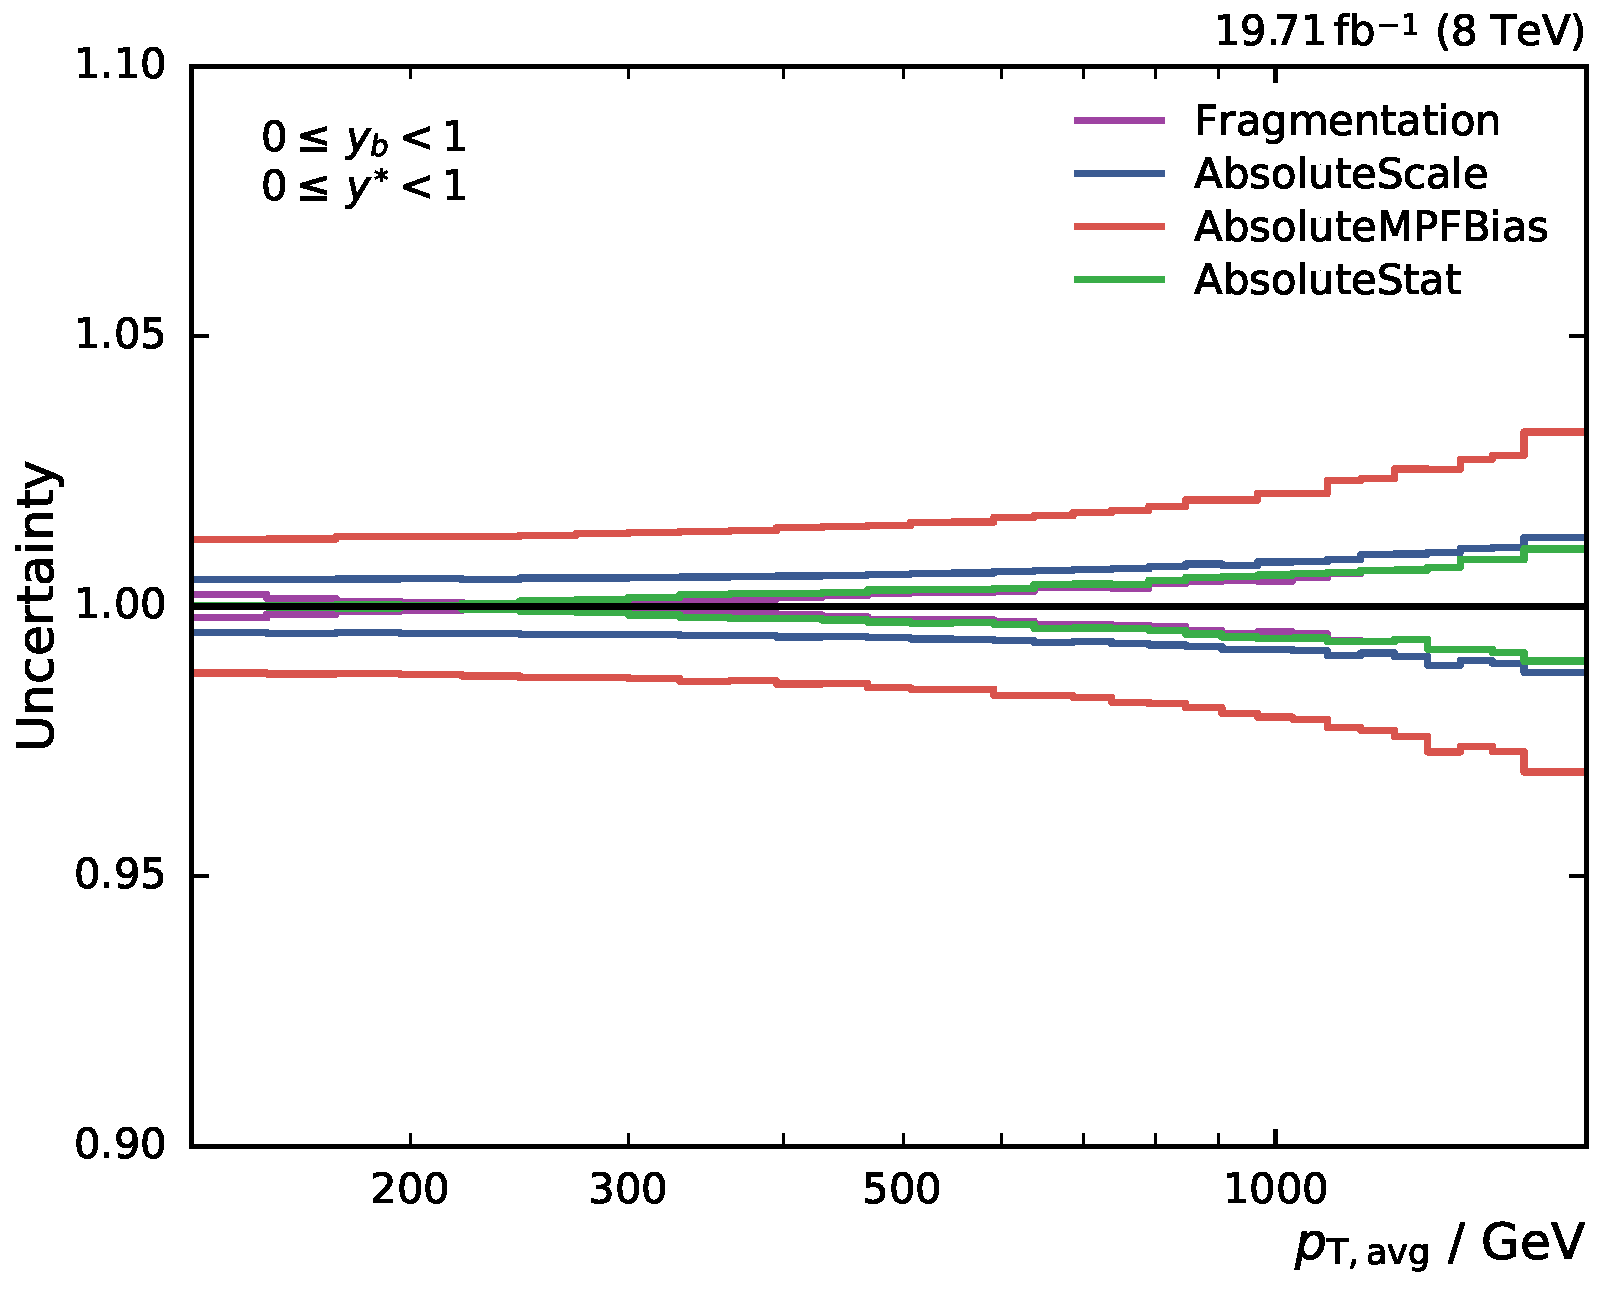
\includegraphics[width=0.49\textwidth]{figures/measurement/jec_relunc_0_yb0ys0.pdf}\hfill
    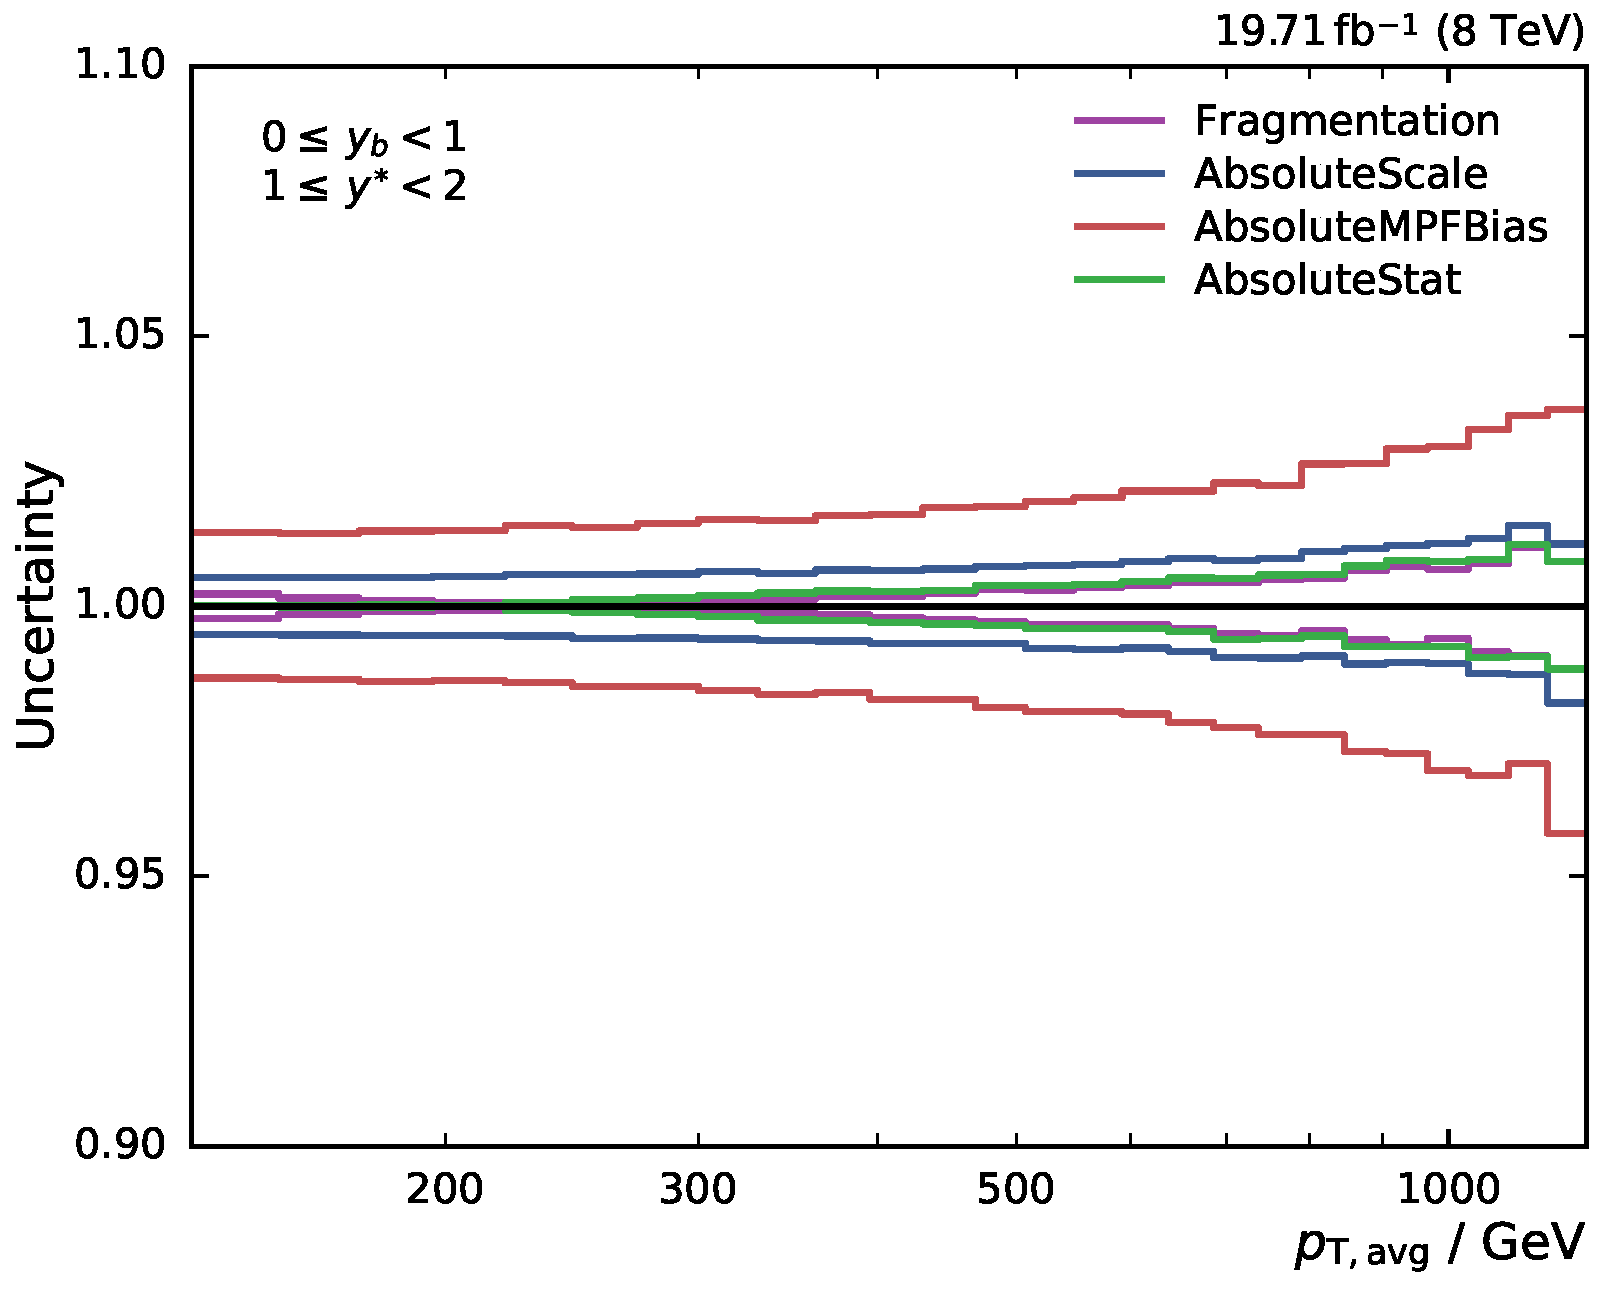
\includegraphics[width=0.49\textwidth]{figures/measurement/jec_relunc_0_yb0ys1.pdf}
    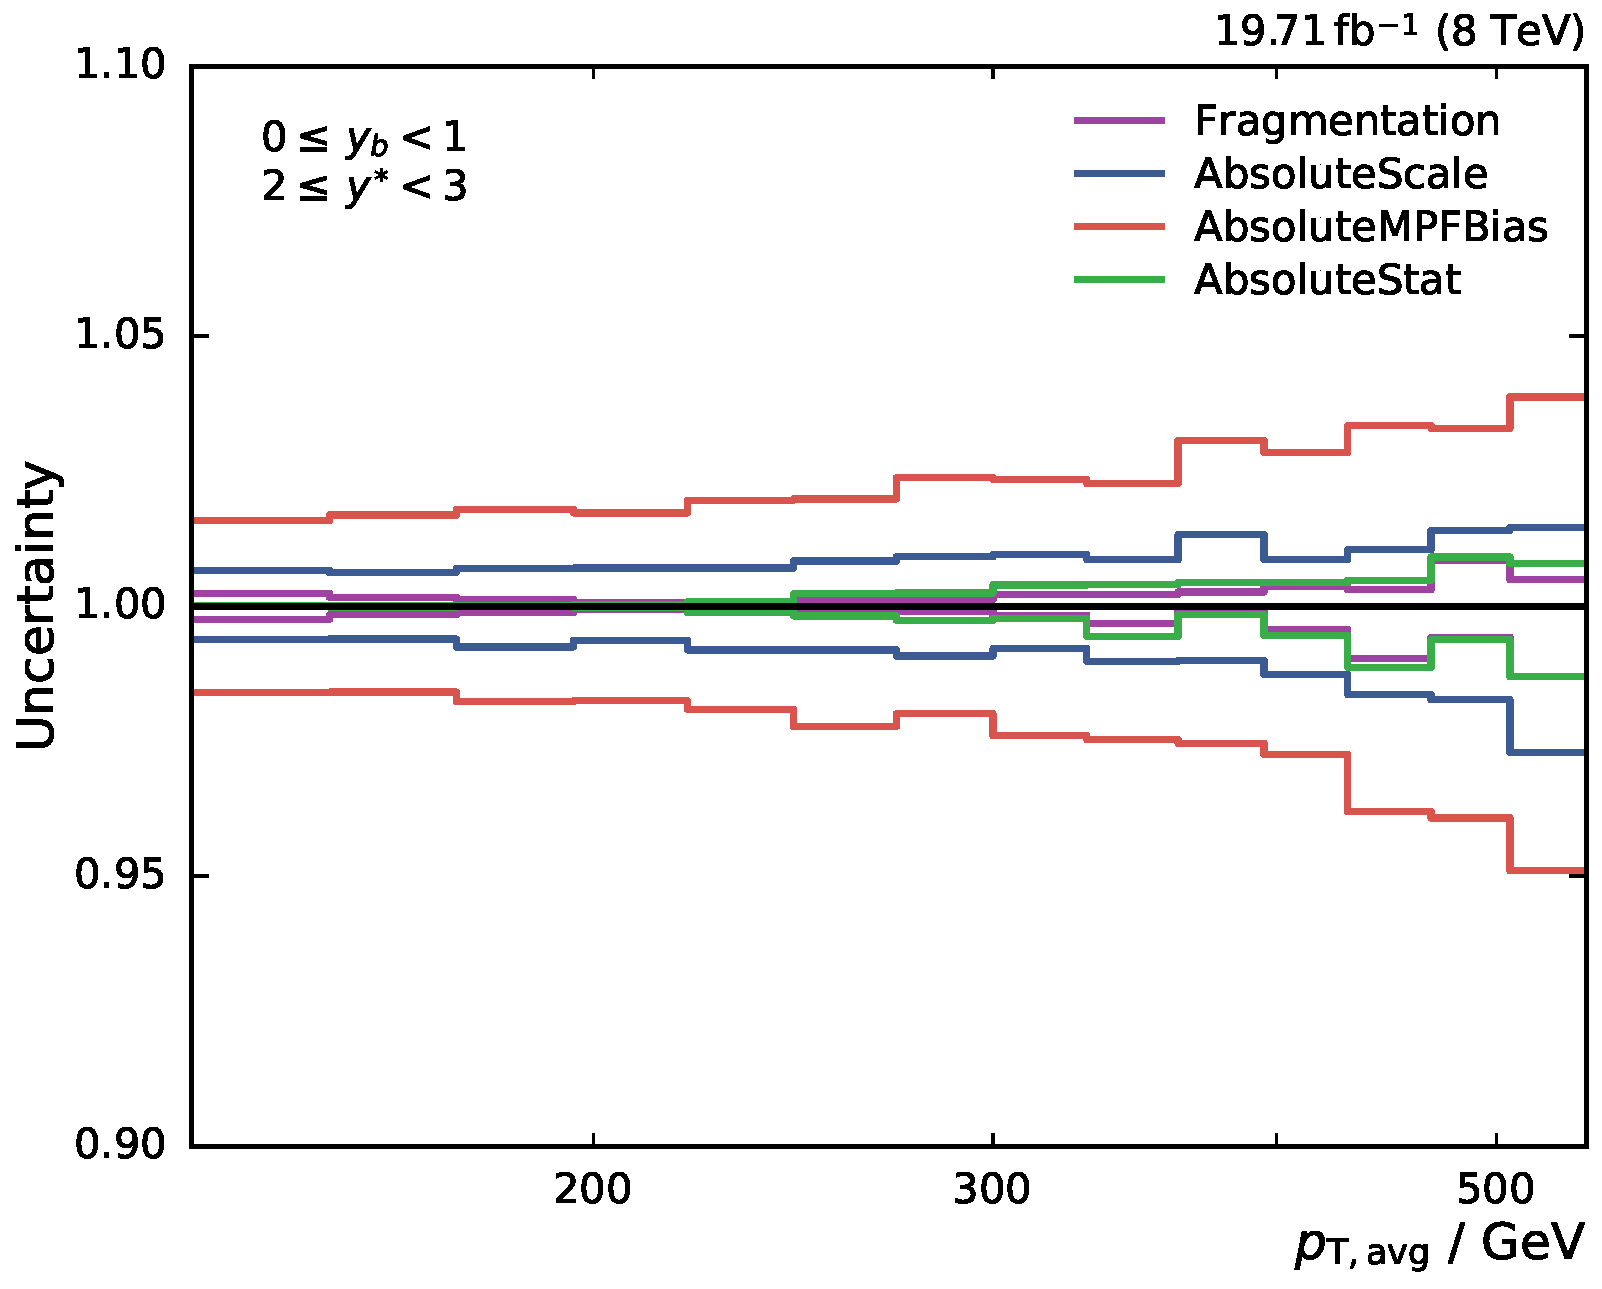
\includegraphics[width=0.49\textwidth]{figures/measurement/jec_relunc_0_yb0ys2.pdf}\hfill
    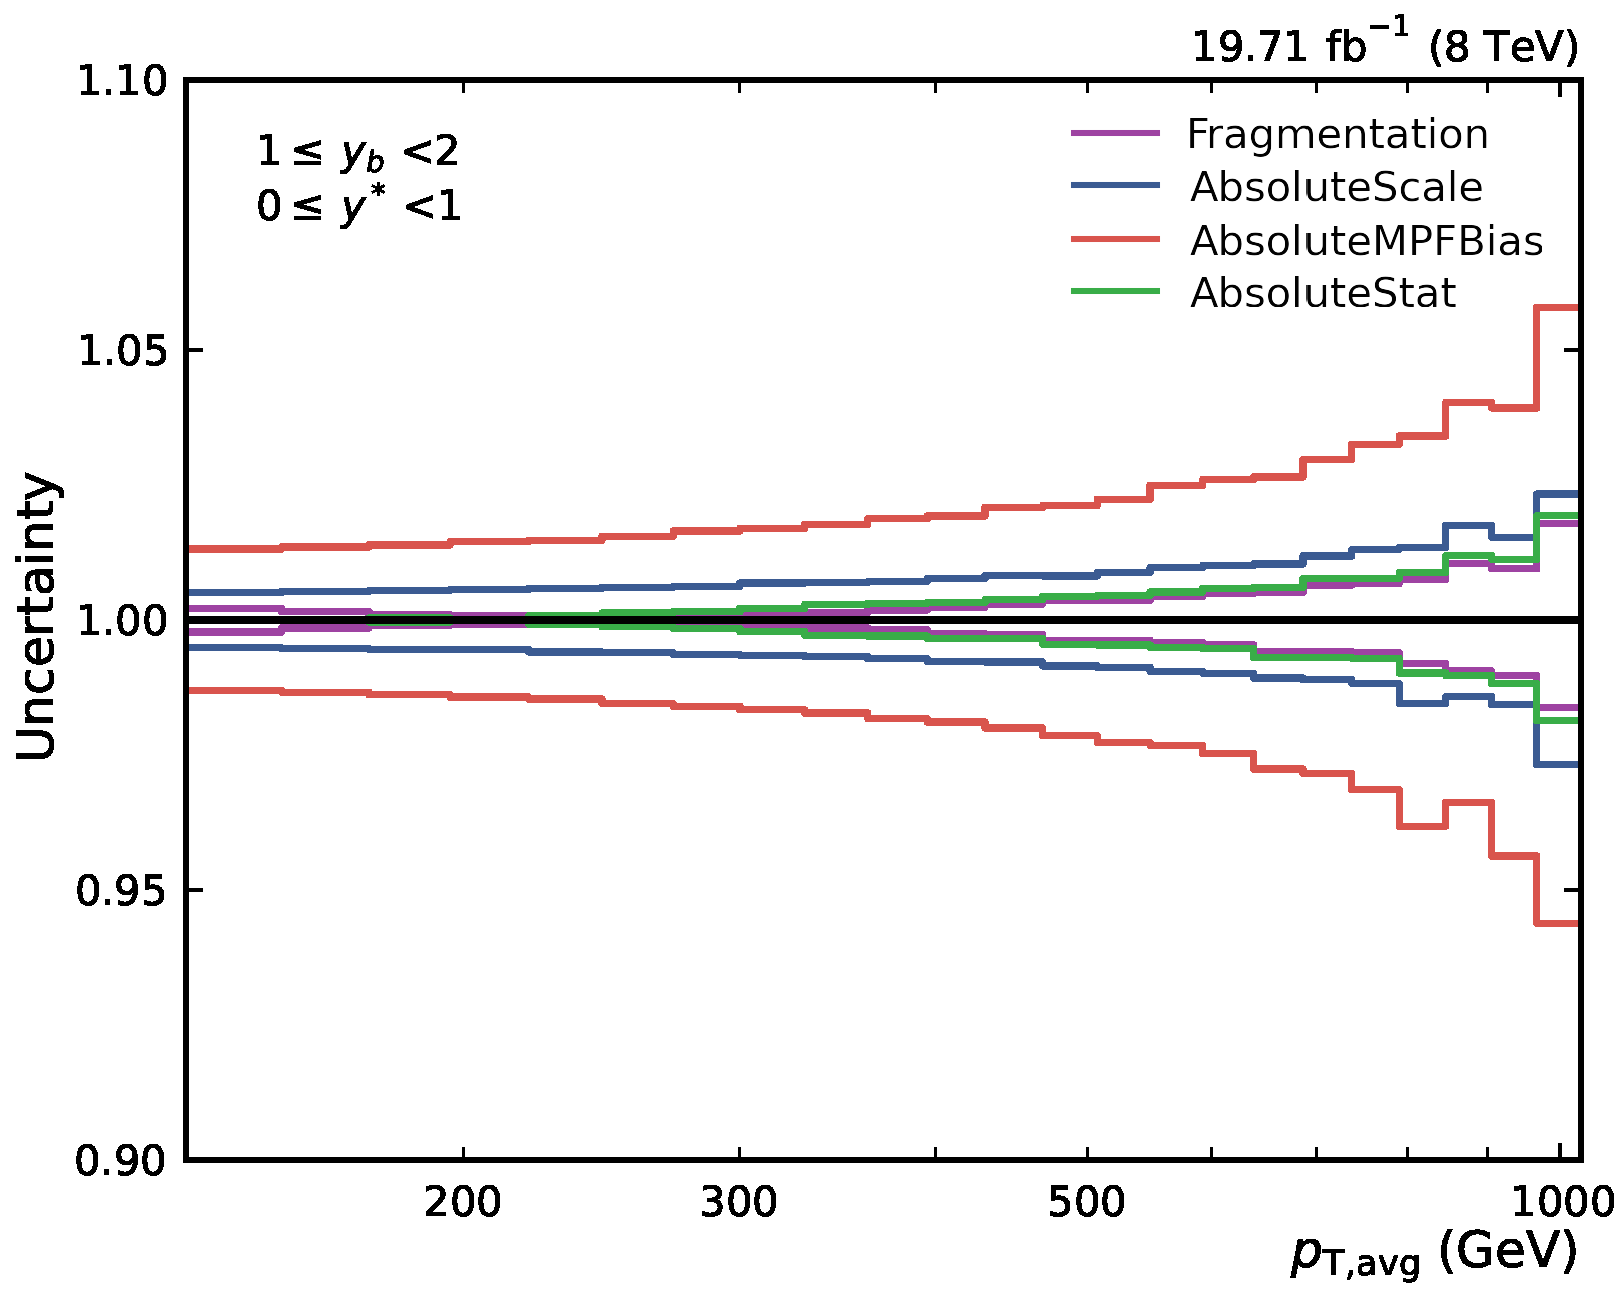
\includegraphics[width=0.49\textwidth]{figures/measurement/jec_relunc_0_yb1ys0.pdf}
    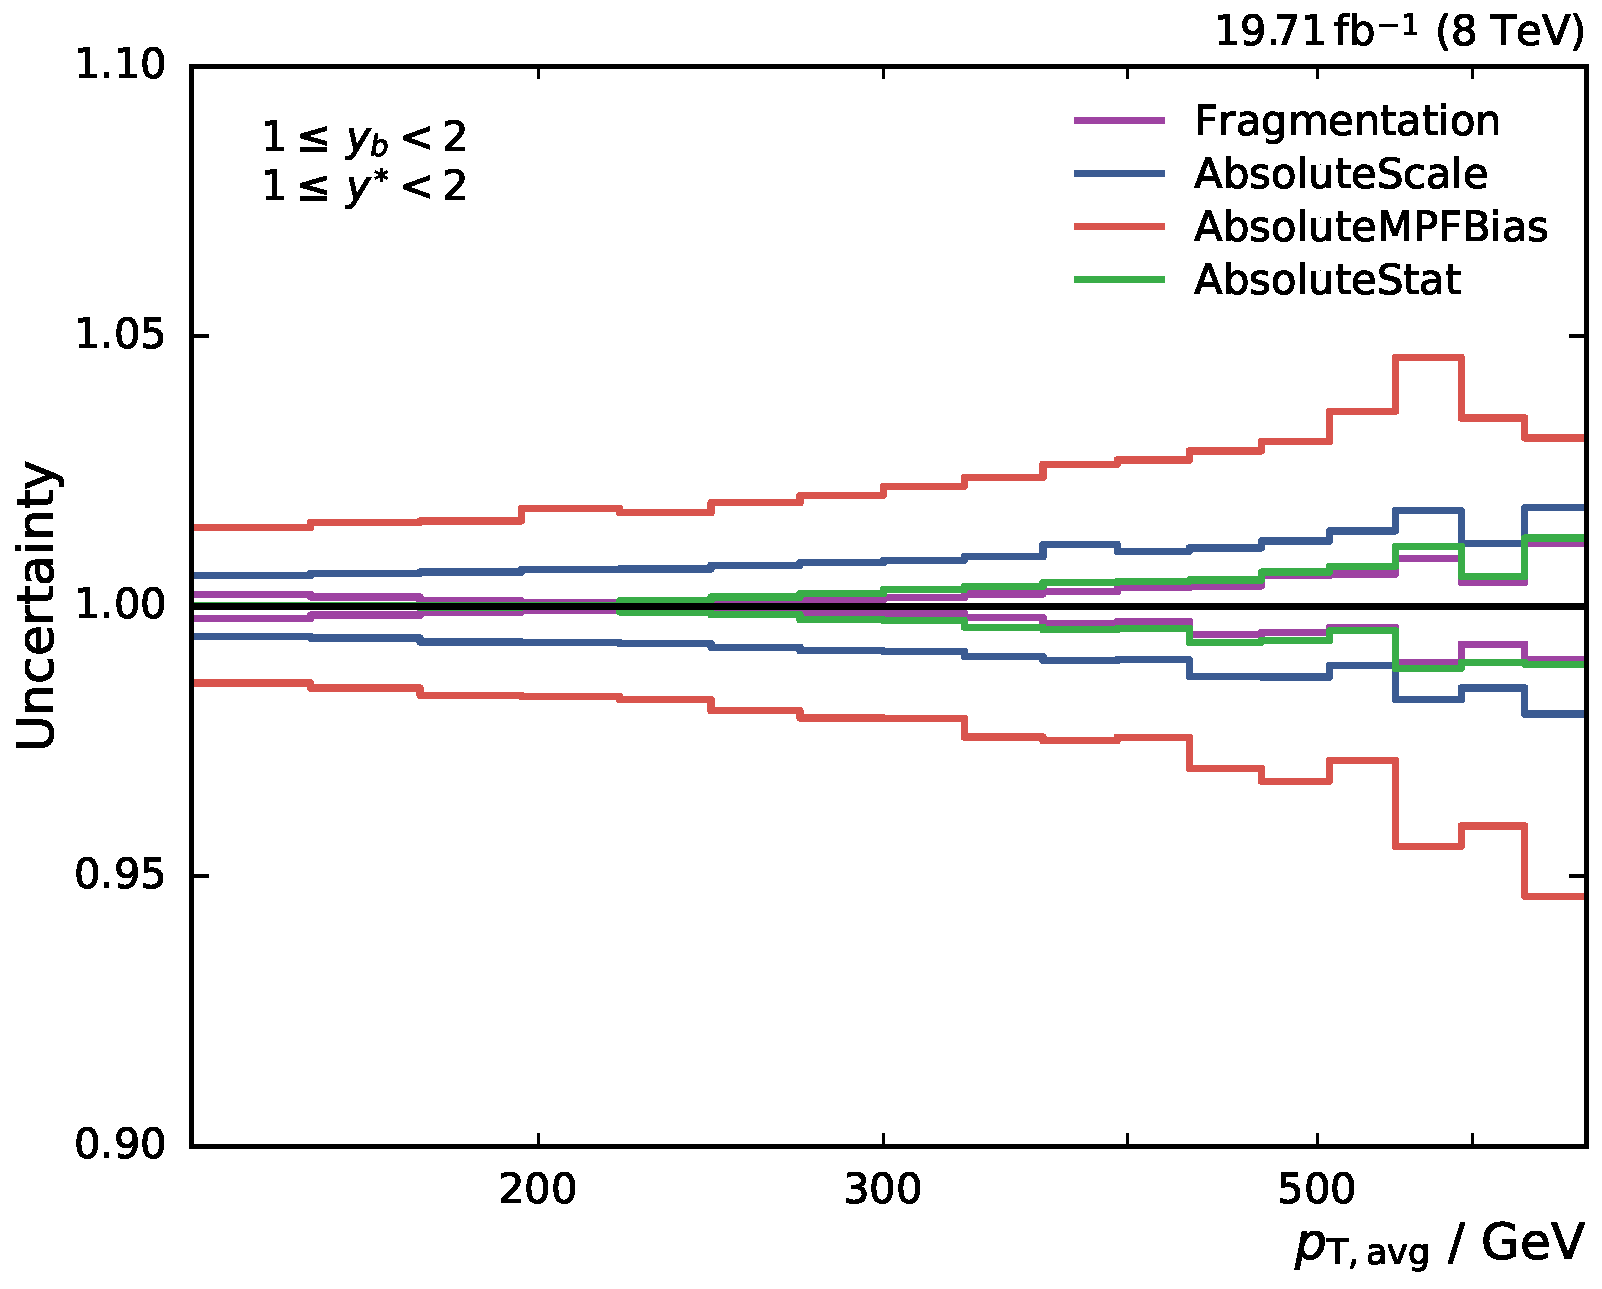
\includegraphics[width=0.49\textwidth]{figures/measurement/jec_relunc_0_yb1ys1.pdf}\hfill
    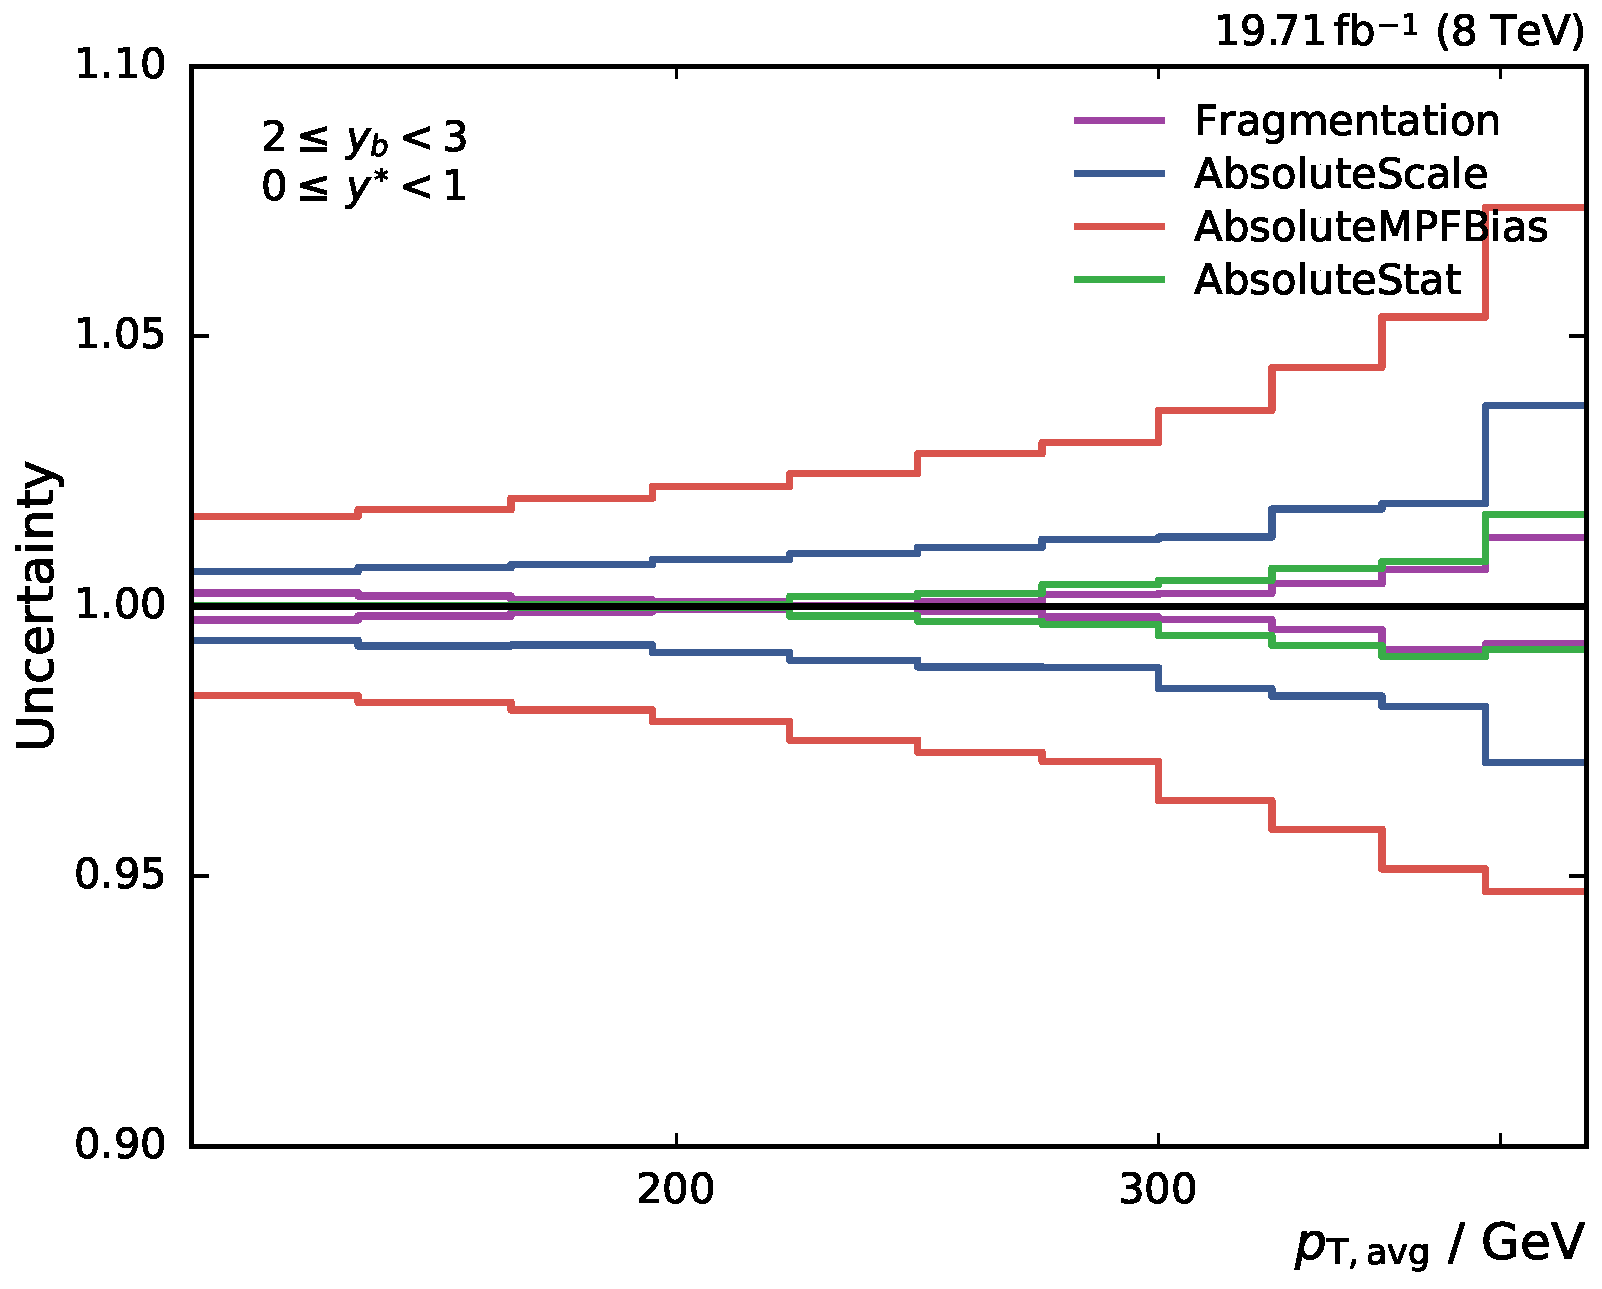
\includegraphics[width=0.49\textwidth]{figures/measurement/jec_relunc_0_yb2ys0.pdf}
    \caption[Split-up of JEC uncertainty sources: Part I]{The relative size of the jet energy scale
             uncertainties for the sources Fragmentation, AbsoluteScale,
             AbsoluteMPFBias,
             and AbsoluteStat are shown for all \ystar and \yboost bins.}
\label{fig:jec_relunc_0}
\end{figure}

\begin{figure}[htbp]
    \centering
    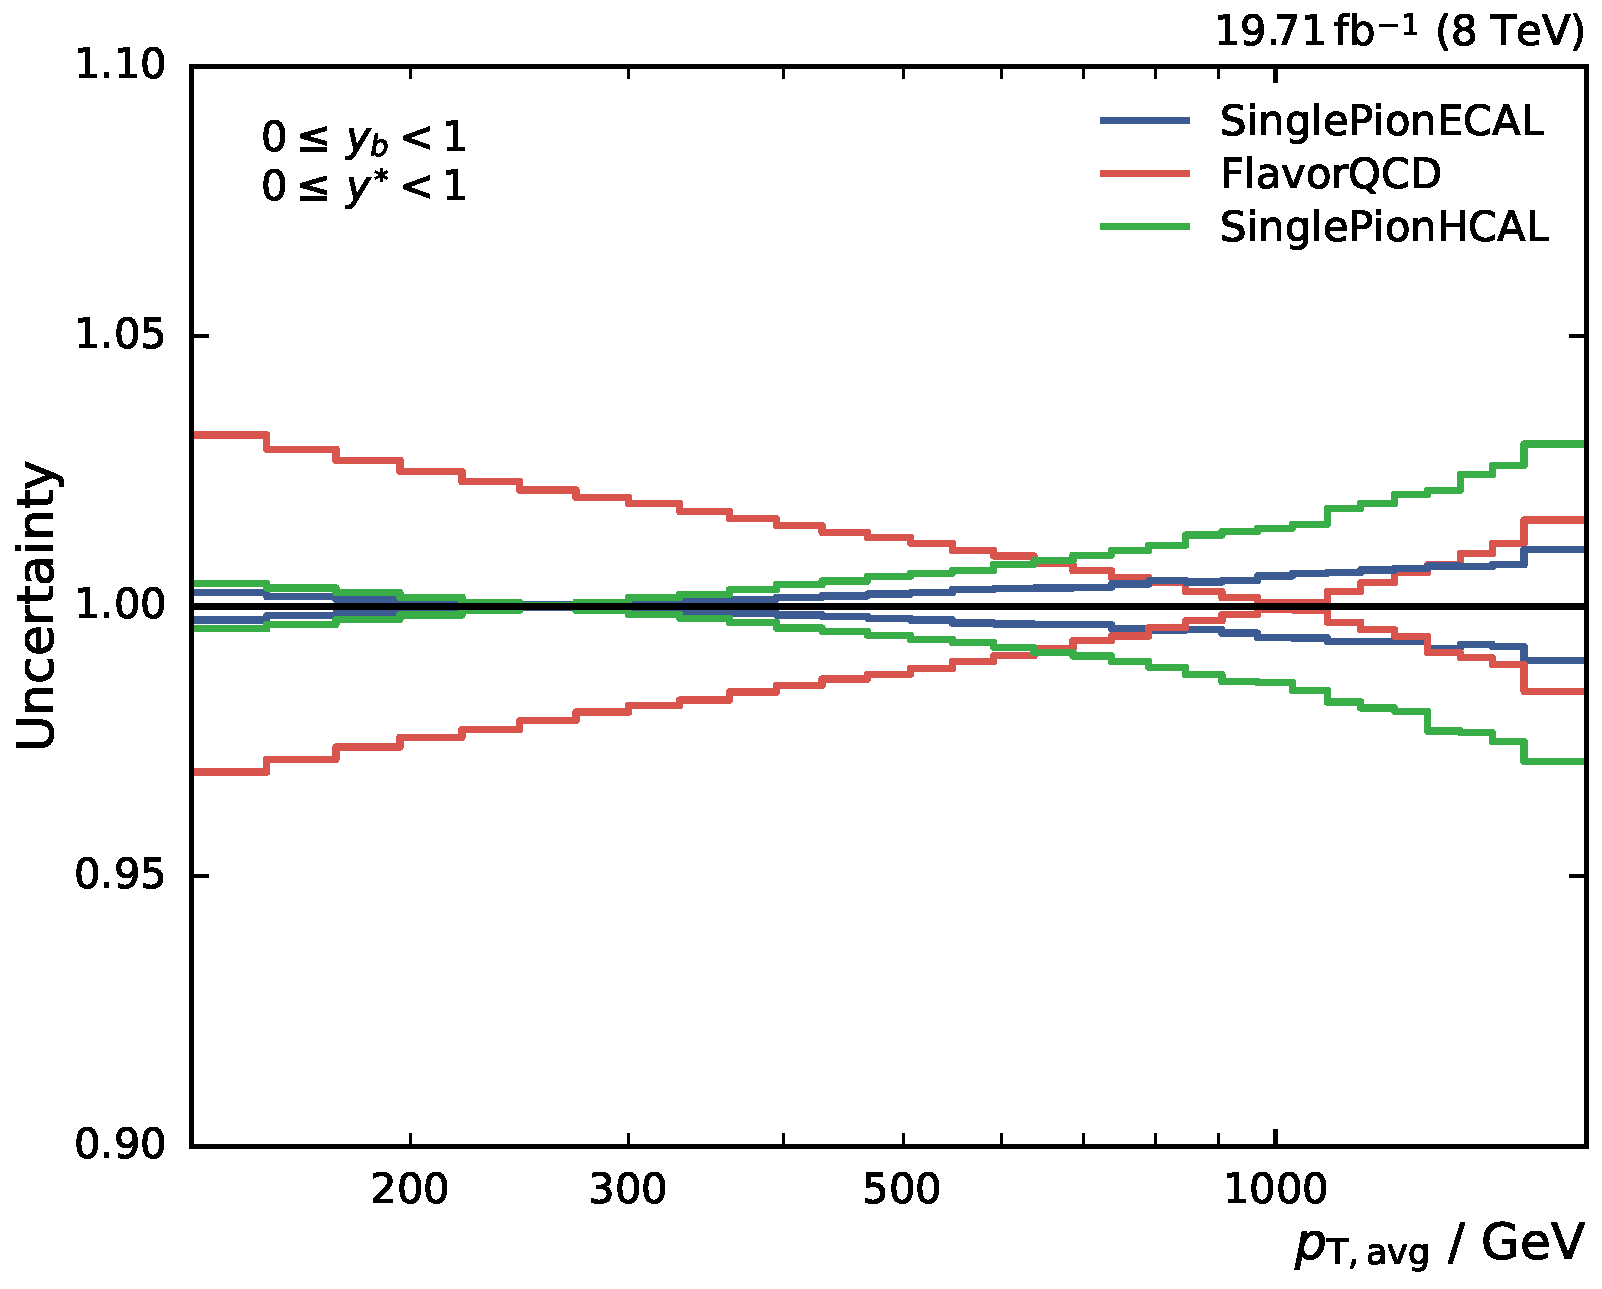
\includegraphics[width=0.49\textwidth]{figures/measurement/jec_relunc_1_yb0ys0.pdf}\hfill
    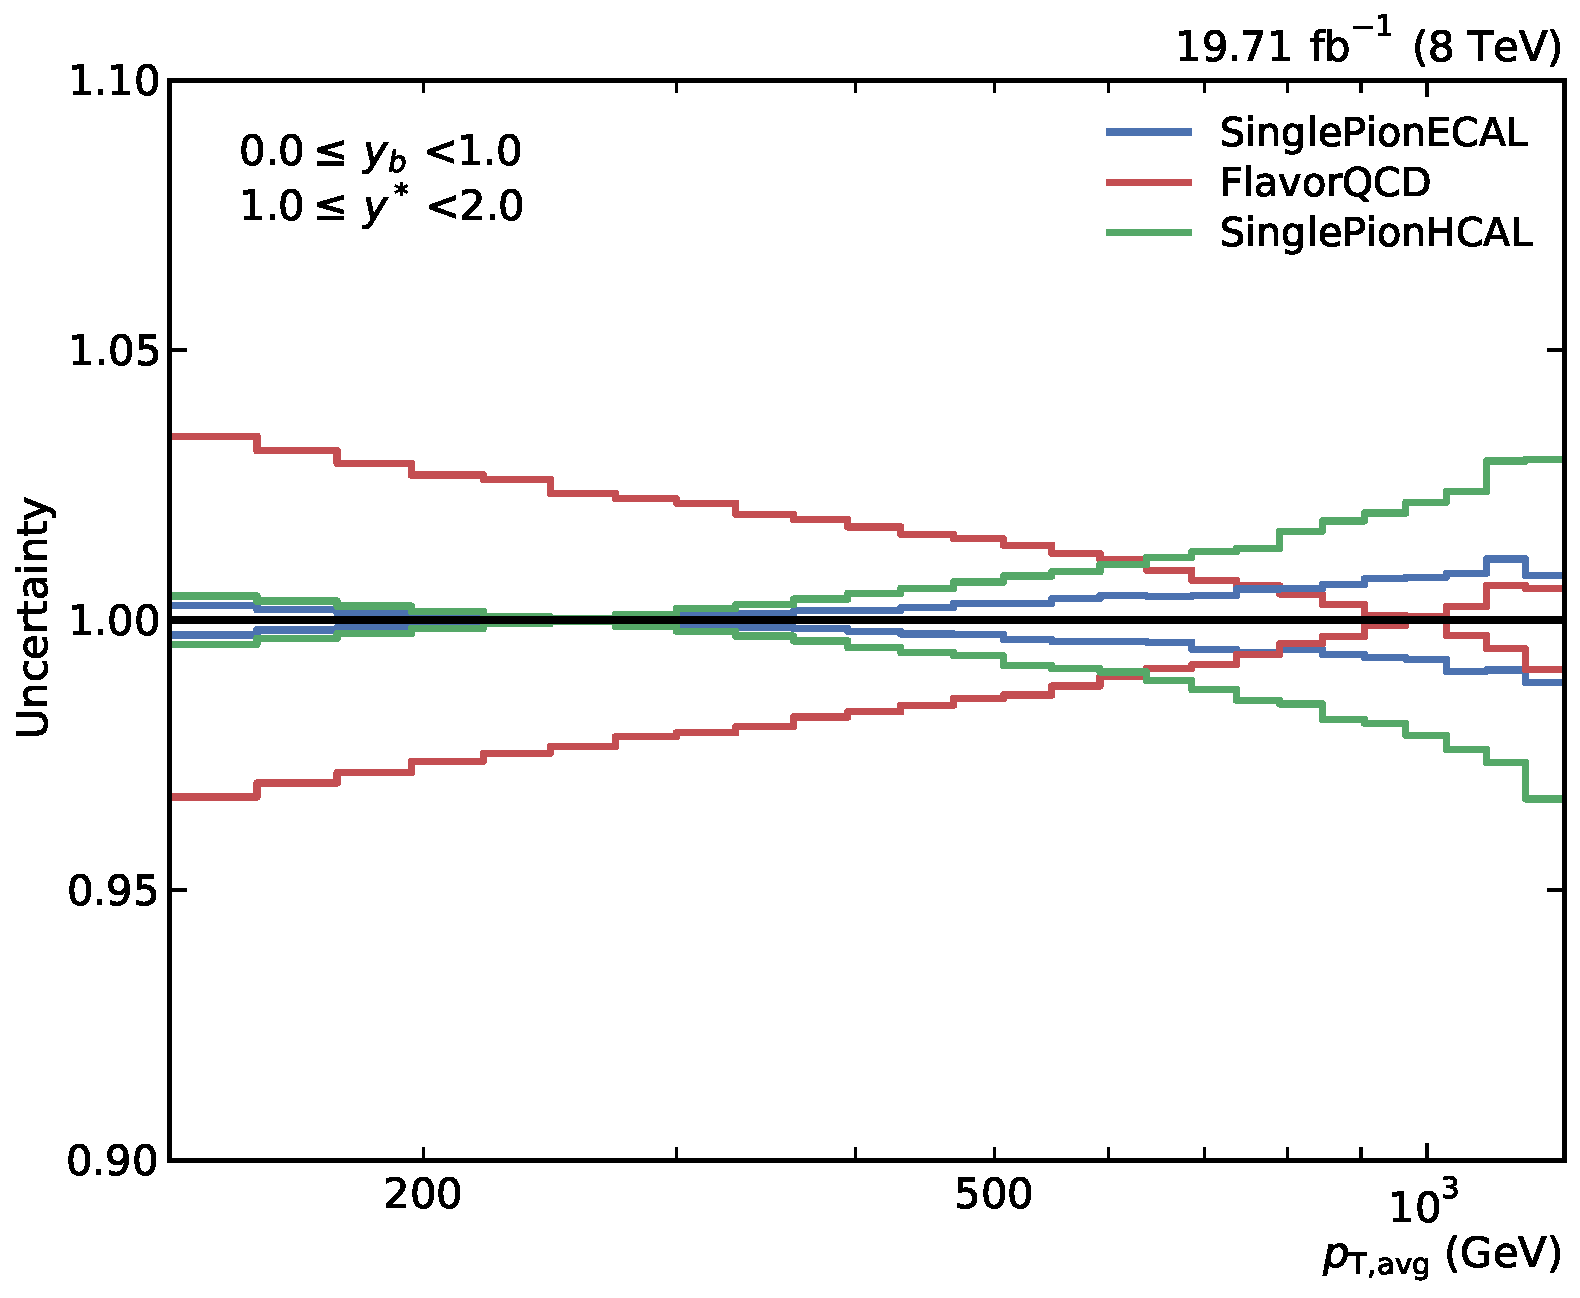
\includegraphics[width=0.49\textwidth]{figures/measurement/jec_relunc_1_yb0ys1.pdf}
    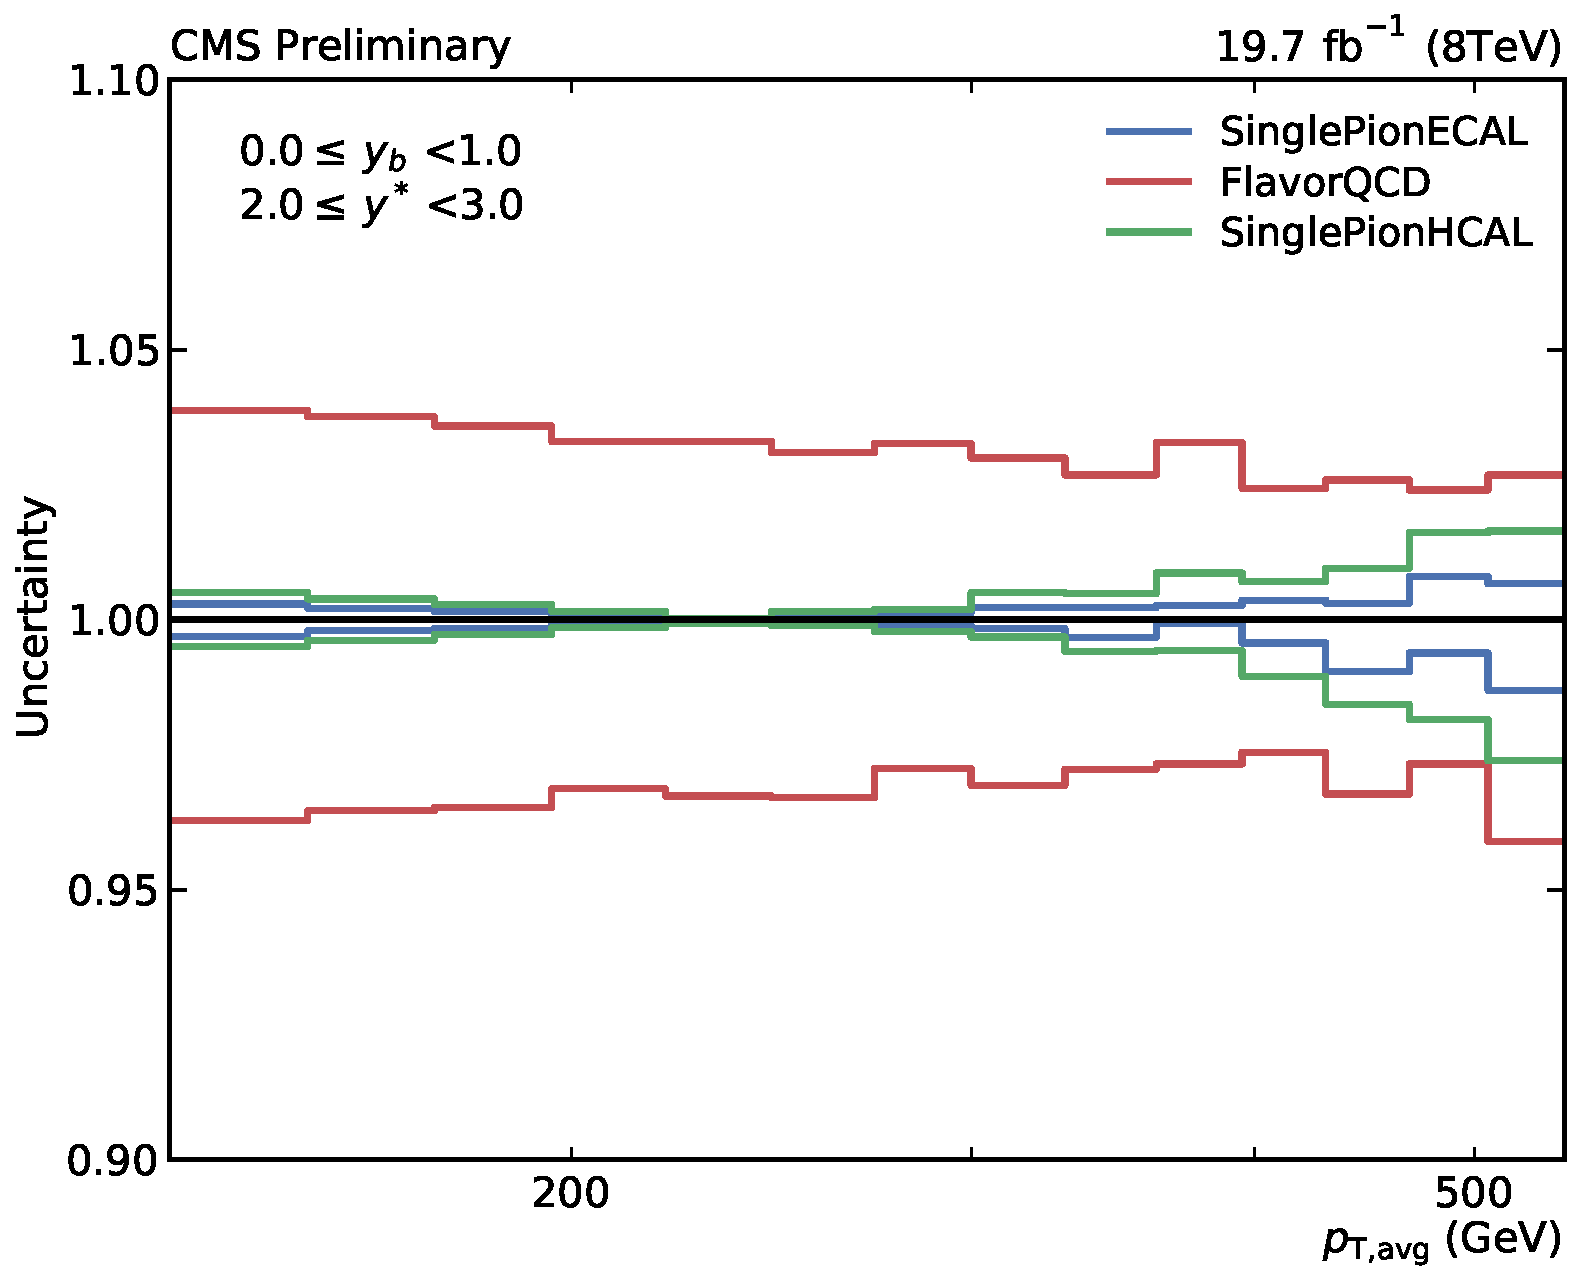
\includegraphics[width=0.49\textwidth]{figures/measurement/jec_relunc_1_yb0ys2.pdf}\hfill
    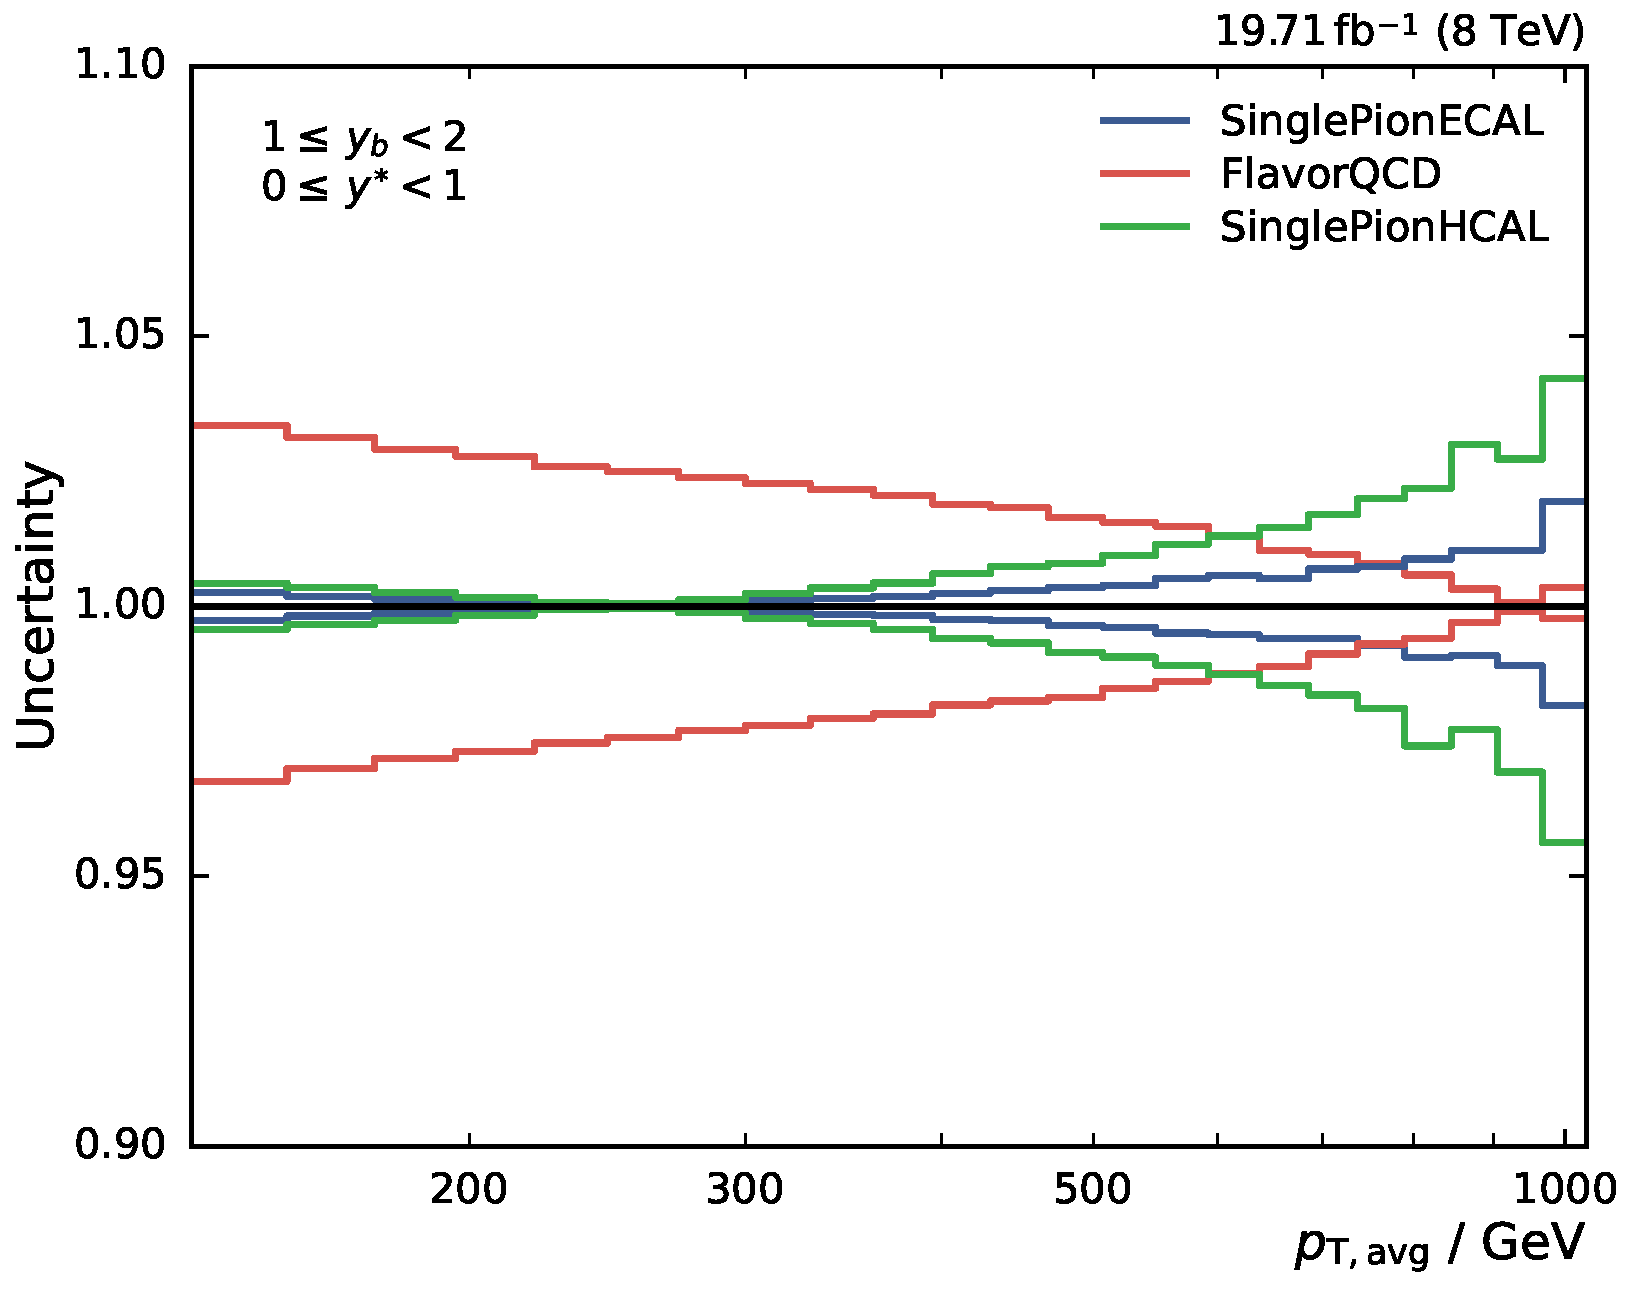
\includegraphics[width=0.49\textwidth]{figures/measurement/jec_relunc_1_yb1ys0.pdf}
    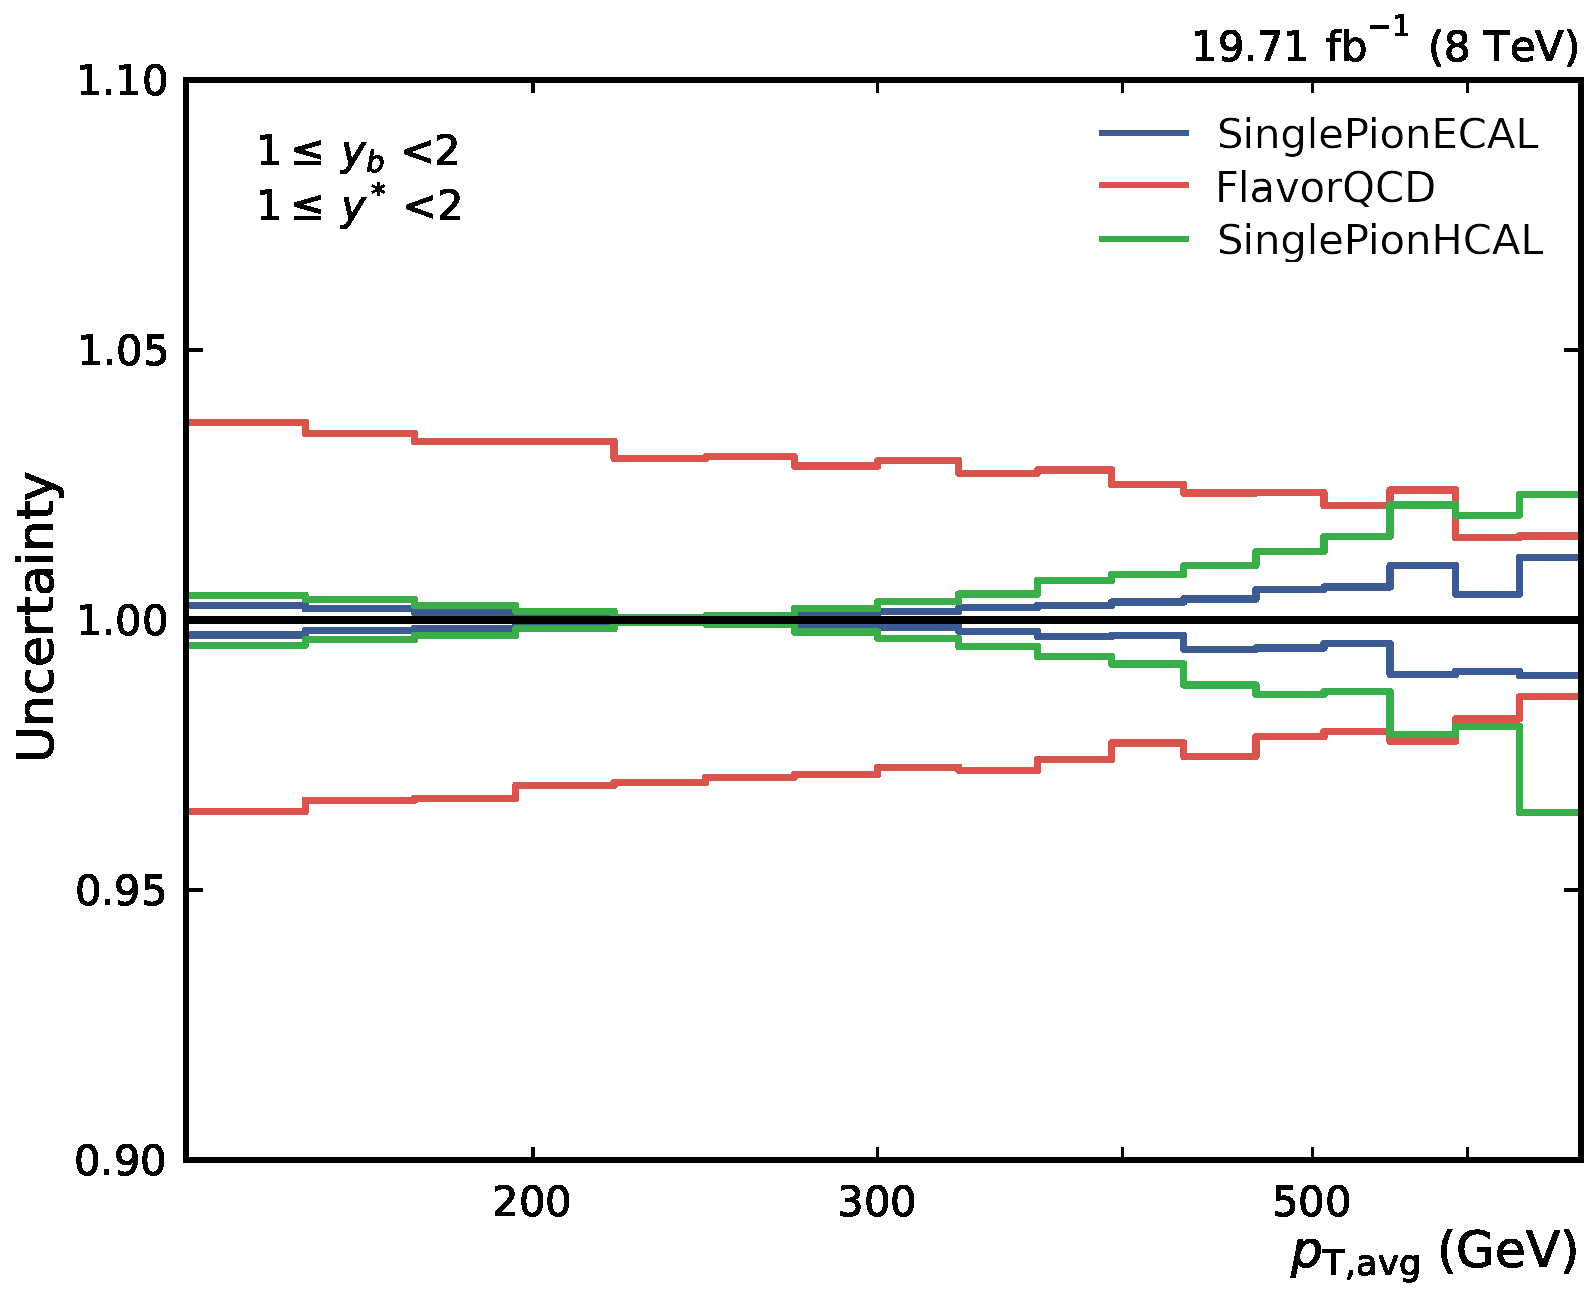
\includegraphics[width=0.49\textwidth]{figures/measurement/jec_relunc_1_yb1ys1.pdf}\hfill
    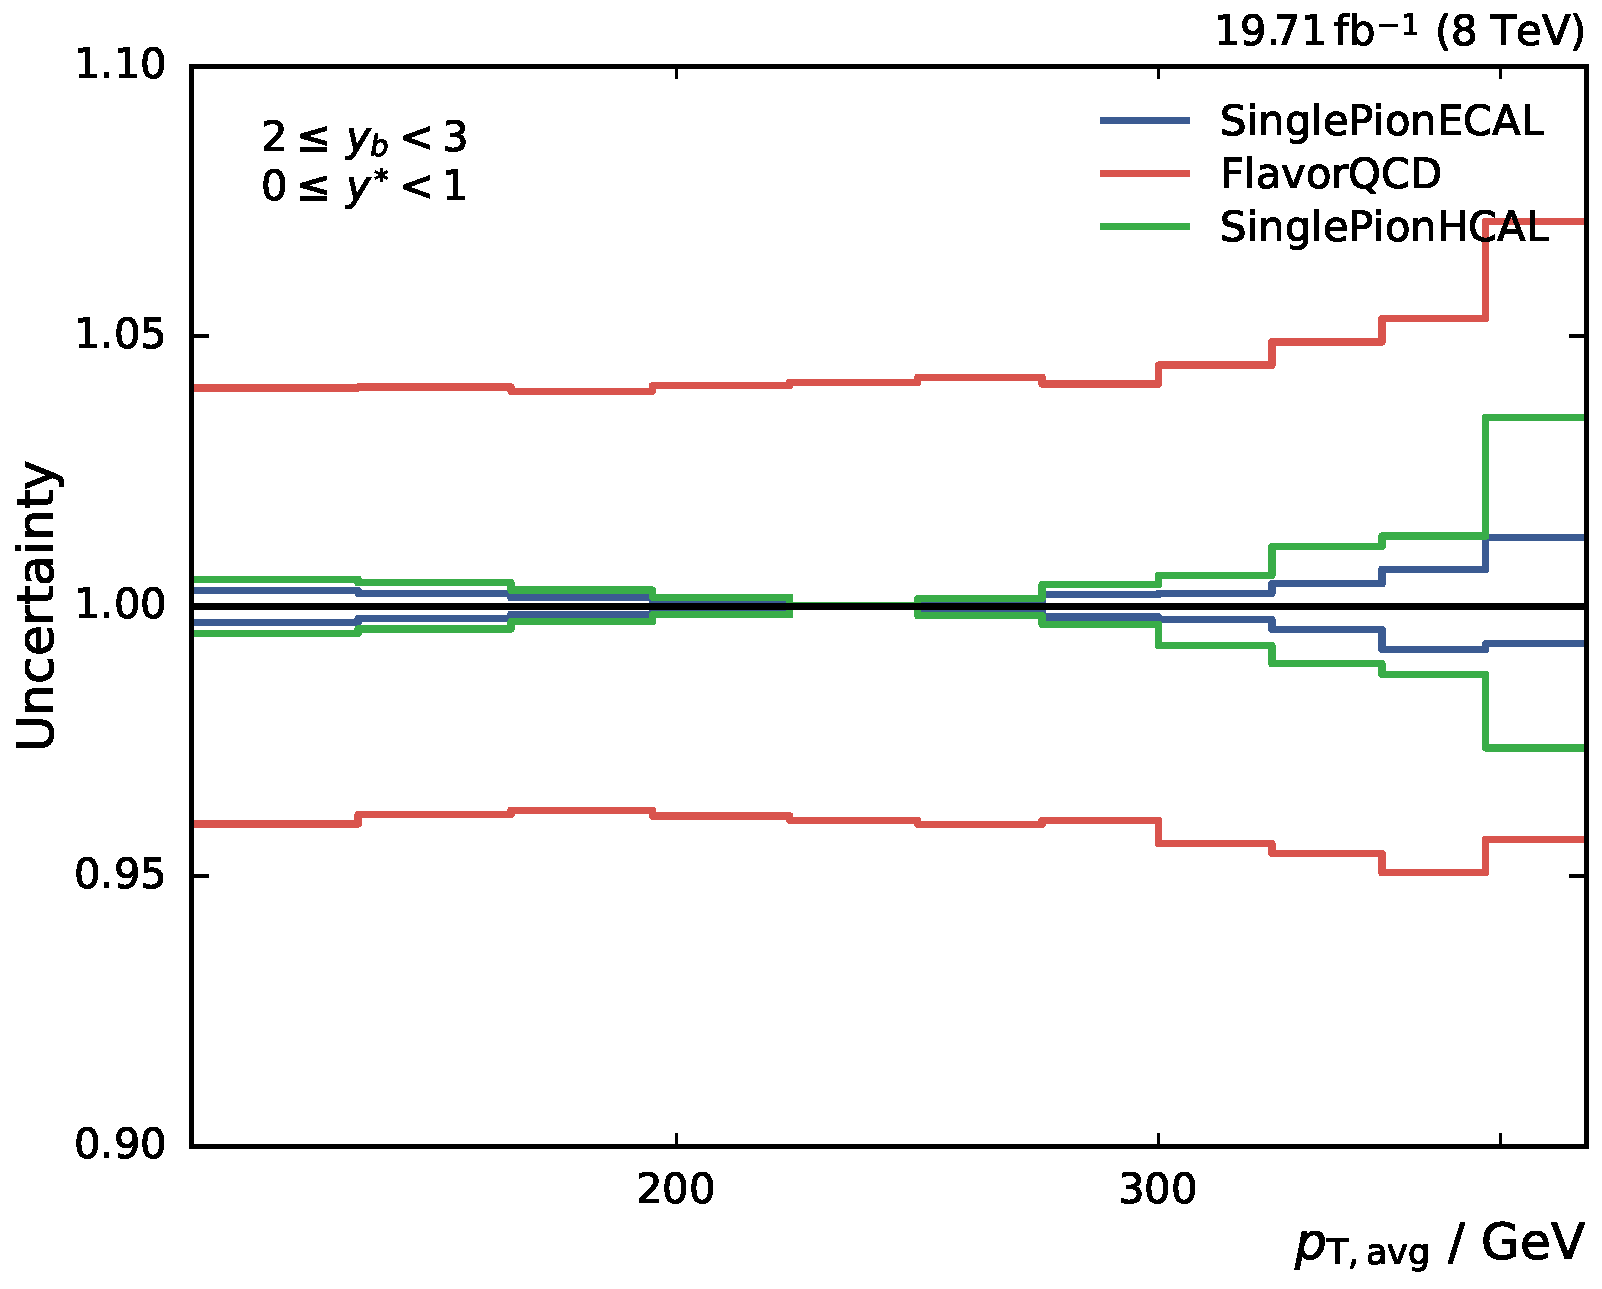
\includegraphics[width=0.49\textwidth]{figures/measurement/jec_relunc_1_yb2ys0.pdf}
    \caption[Split-up of JEC uncertainty sources: Part II] {The relative size of the jet energy scale
             uncertainties for the sources SinglePionECAL, SinglePionHCAL, and
             FlavorQCD are shown for all \ystar and \yboost bins.}
    \label{fig:jec_relunc_1}
\end{figure}

\begin{figure}[htbp]
    \centering
    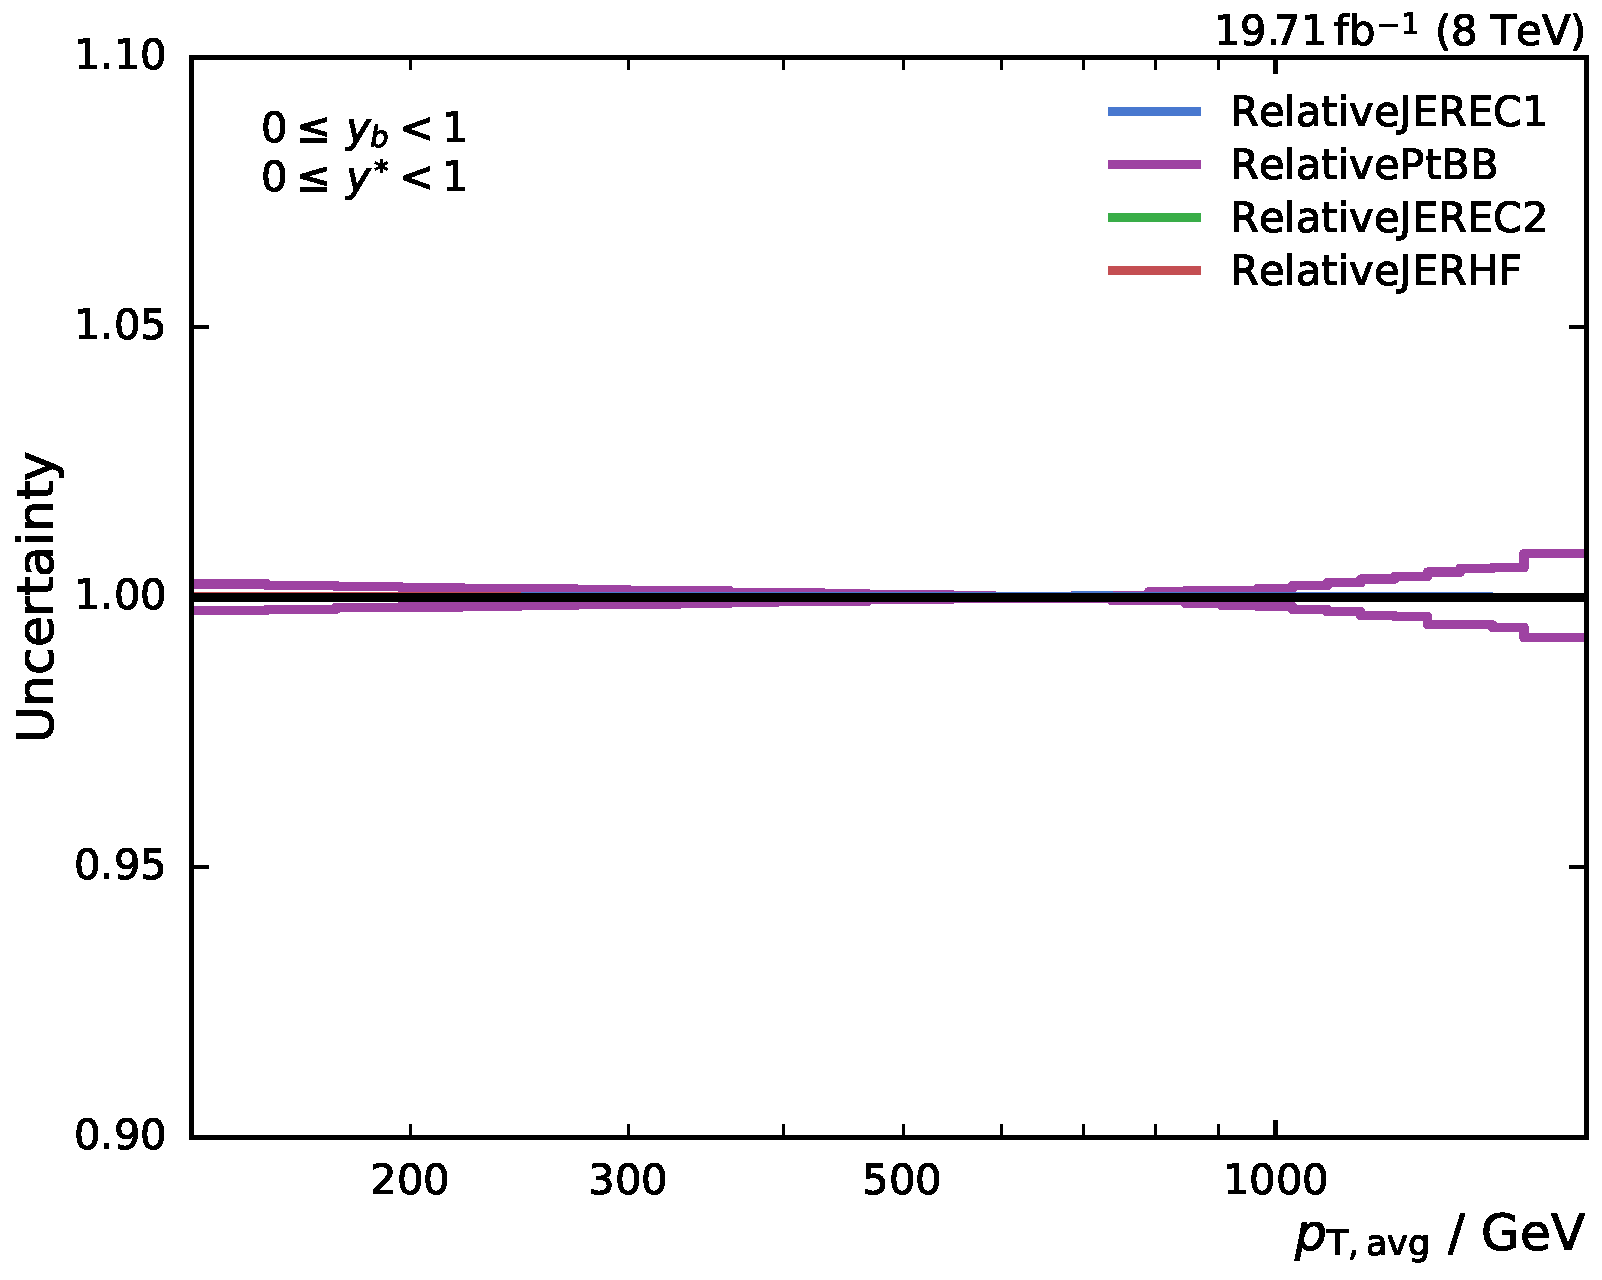
\includegraphics[width=0.49\textwidth]{figures/measurement/jec_relunc_2_yb0ys0.pdf}\hfill
    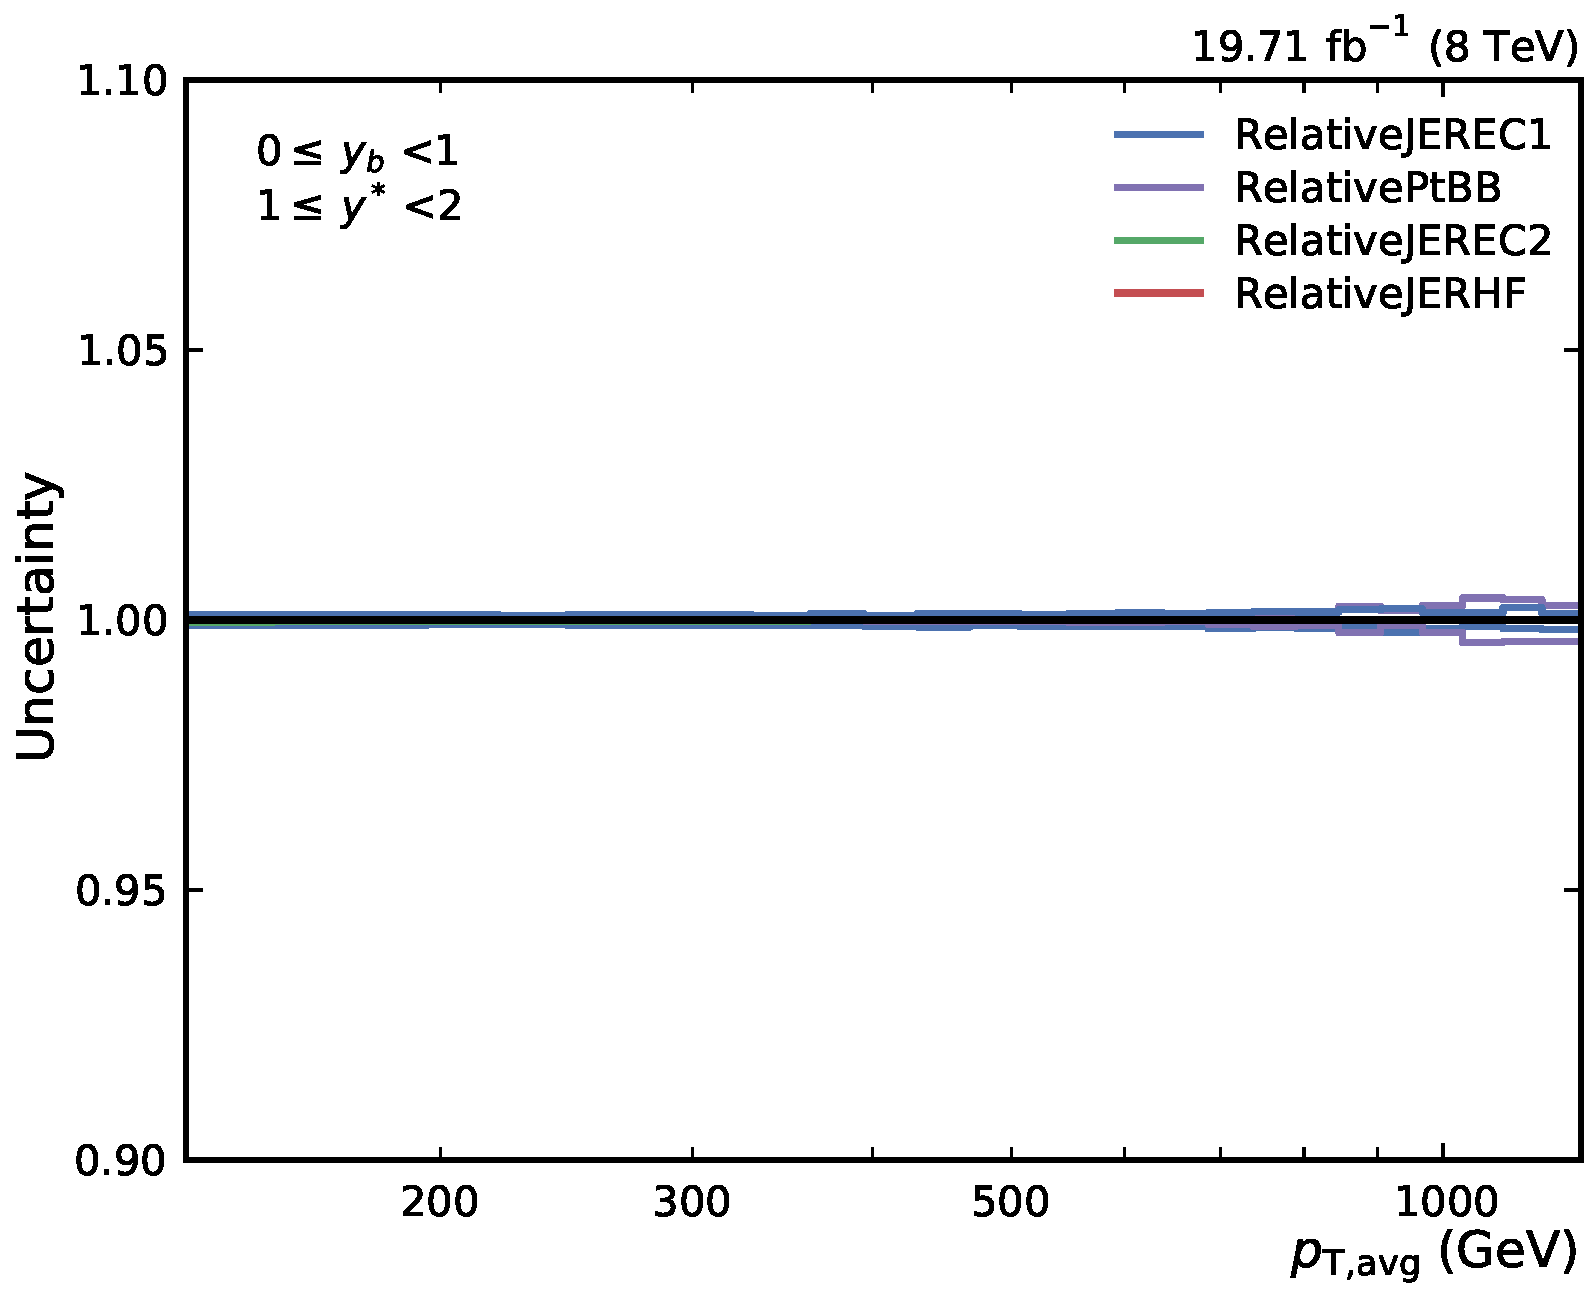
\includegraphics[width=0.49\textwidth]{figures/measurement/jec_relunc_2_yb0ys1.pdf}
    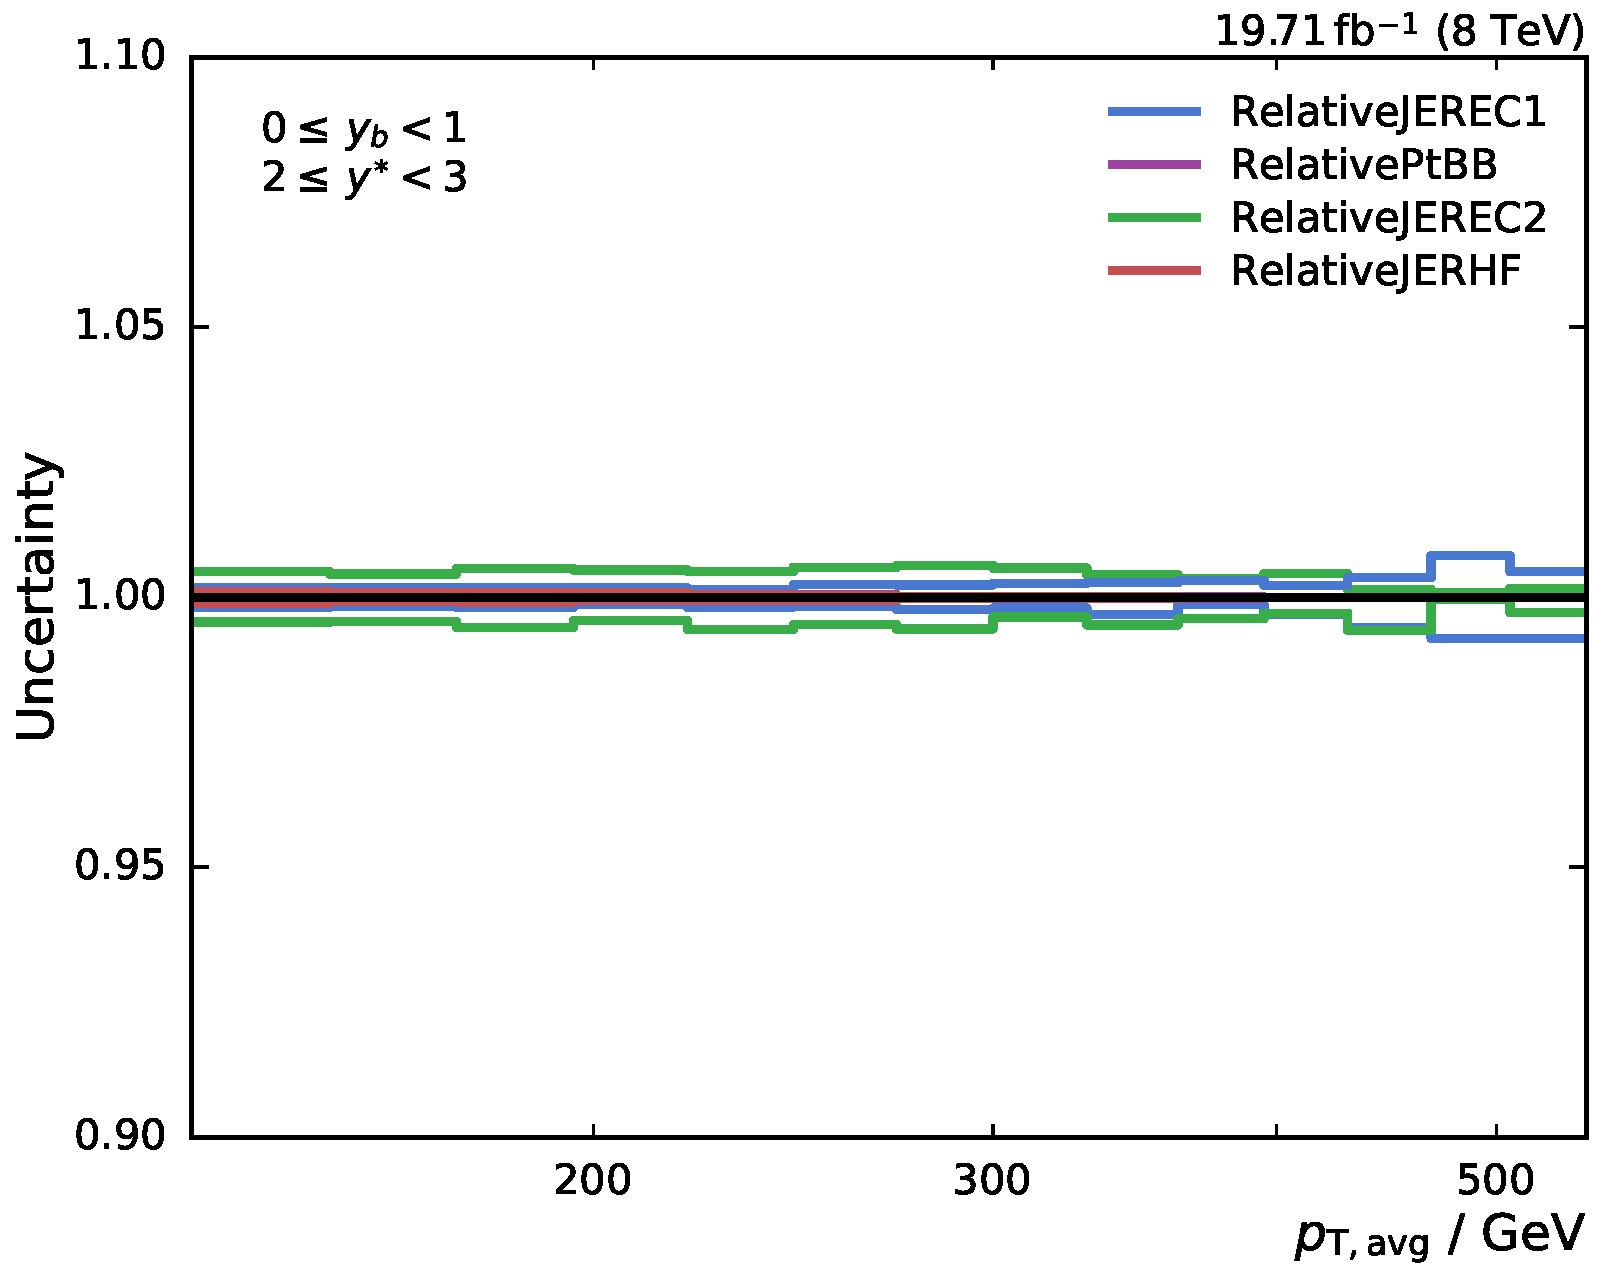
\includegraphics[width=0.49\textwidth]{figures/measurement/jec_relunc_2_yb0ys2.pdf}\hfill
    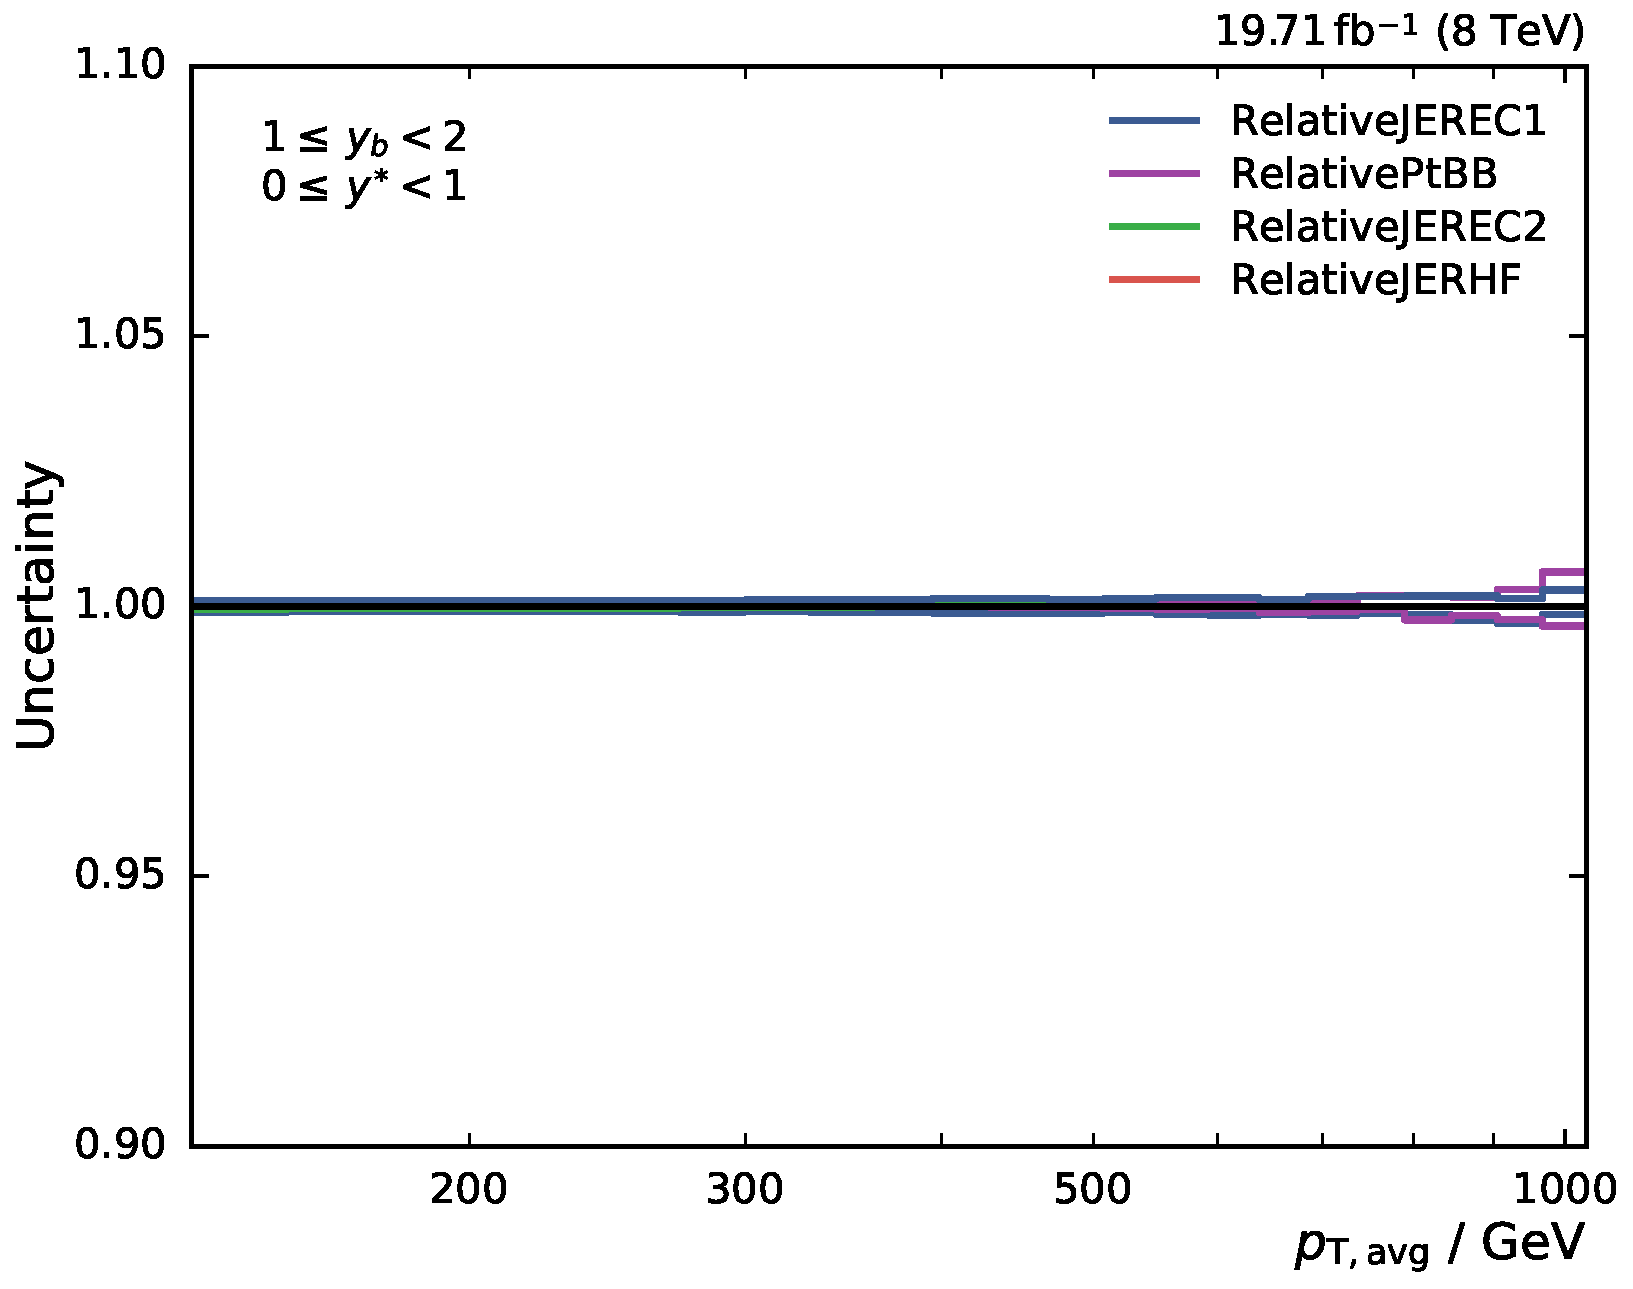
\includegraphics[width=0.49\textwidth]{figures/measurement/jec_relunc_2_yb1ys0.pdf}
    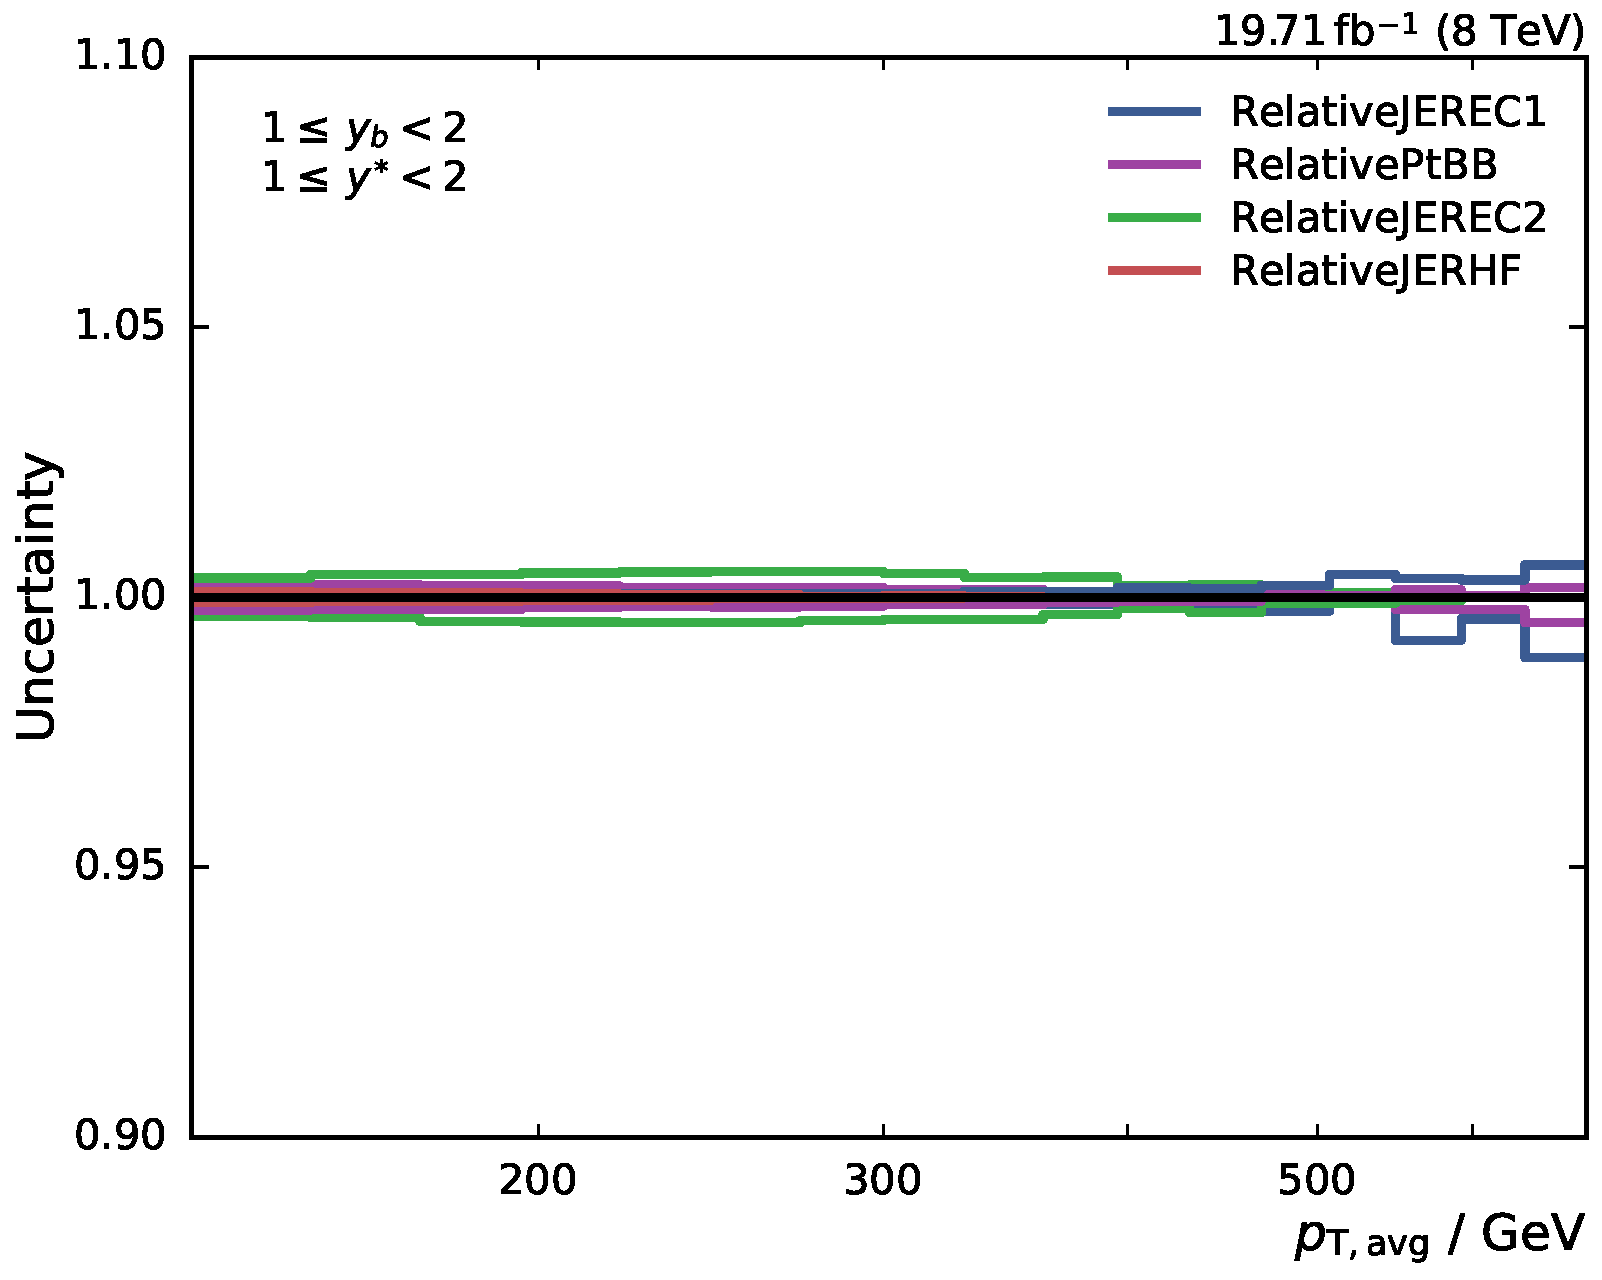
\includegraphics[width=0.49\textwidth]{figures/measurement/jec_relunc_2_yb1ys1.pdf}\hfill
    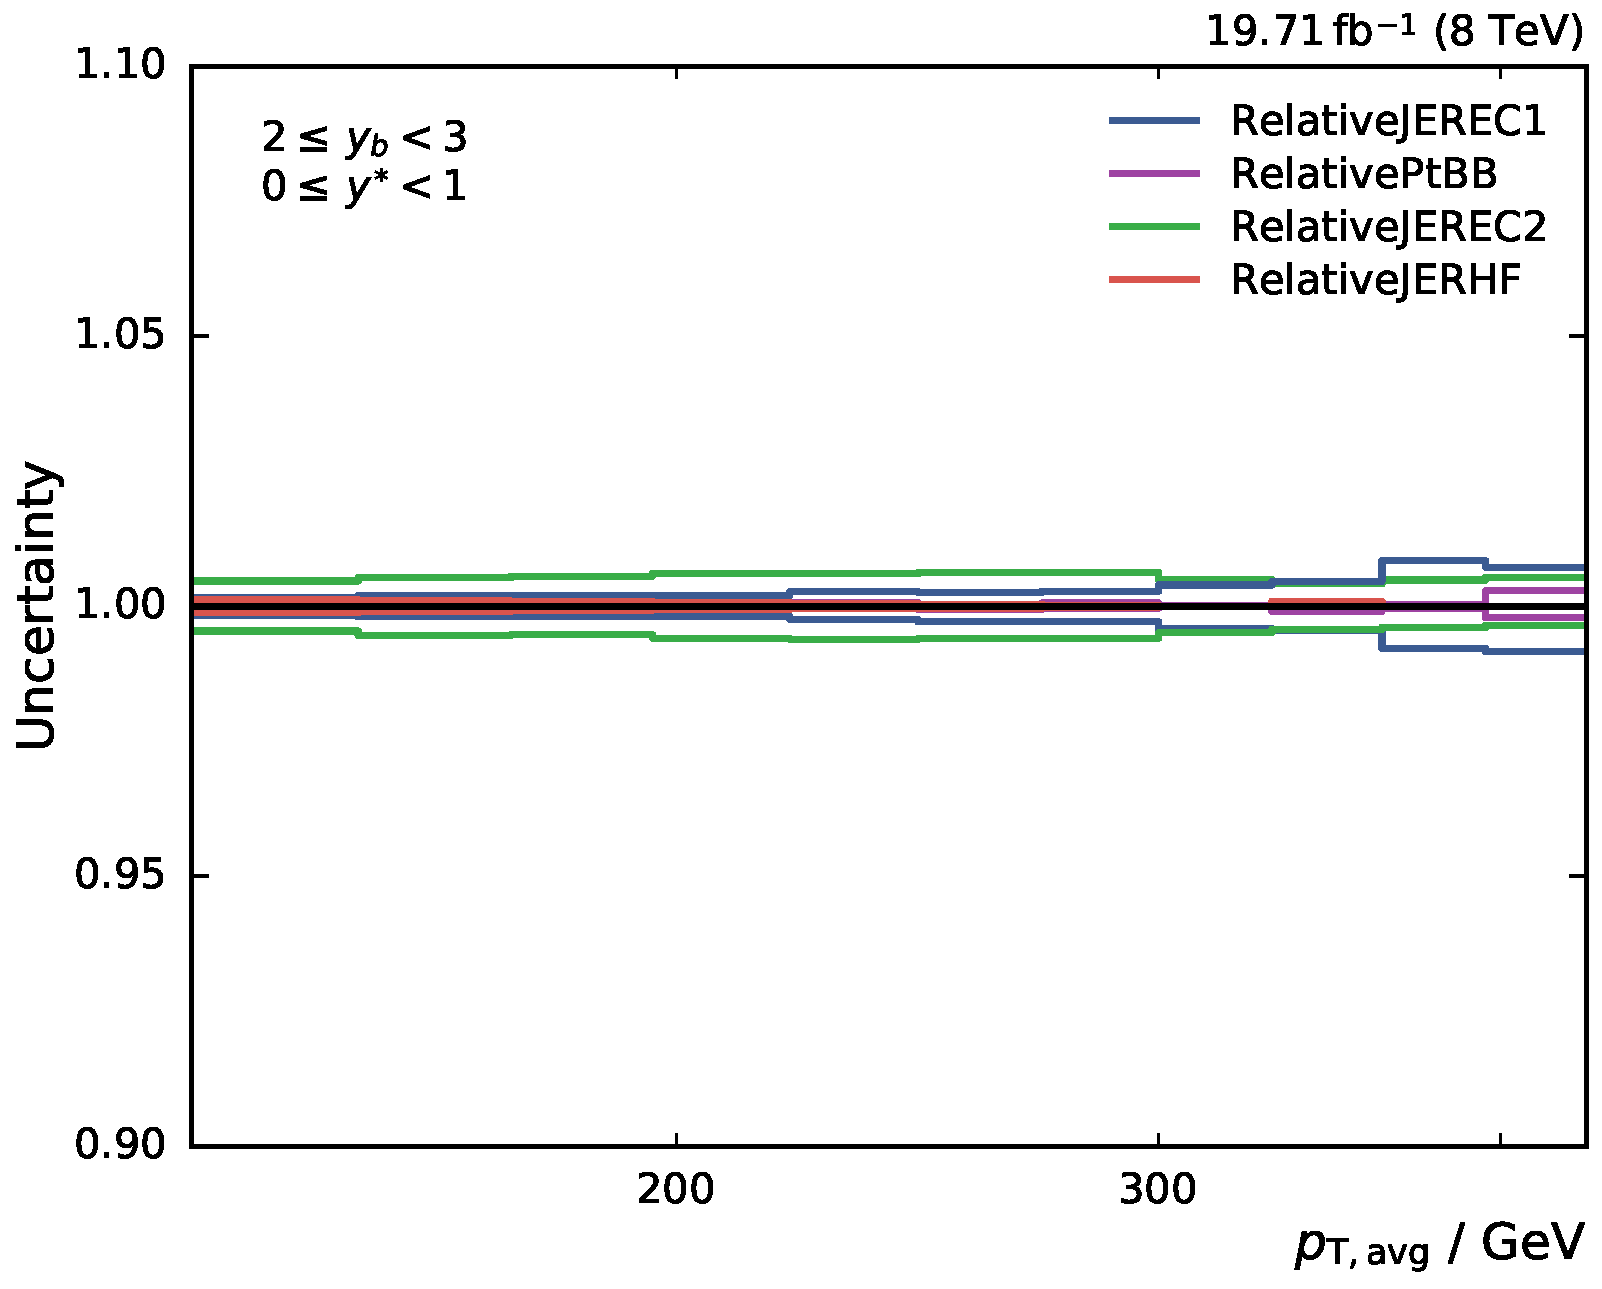
\includegraphics[width=0.49\textwidth]{figures/measurement/jec_relunc_2_yb2ys0.pdf}
    \caption[Split-up of JEC uncertainty sources: Part III] {The relative size of the jet energy scale
             uncertainties for the sources RelativeJEREC1, RelativeJEREC2,
             RelativePtBB, and RelativeJERHF are shown for all \ystar and \yboost bins.}
    \label{fig:jec_relunc_2}
\end{figure}


\begin{figure}[htbp]
    \centering
    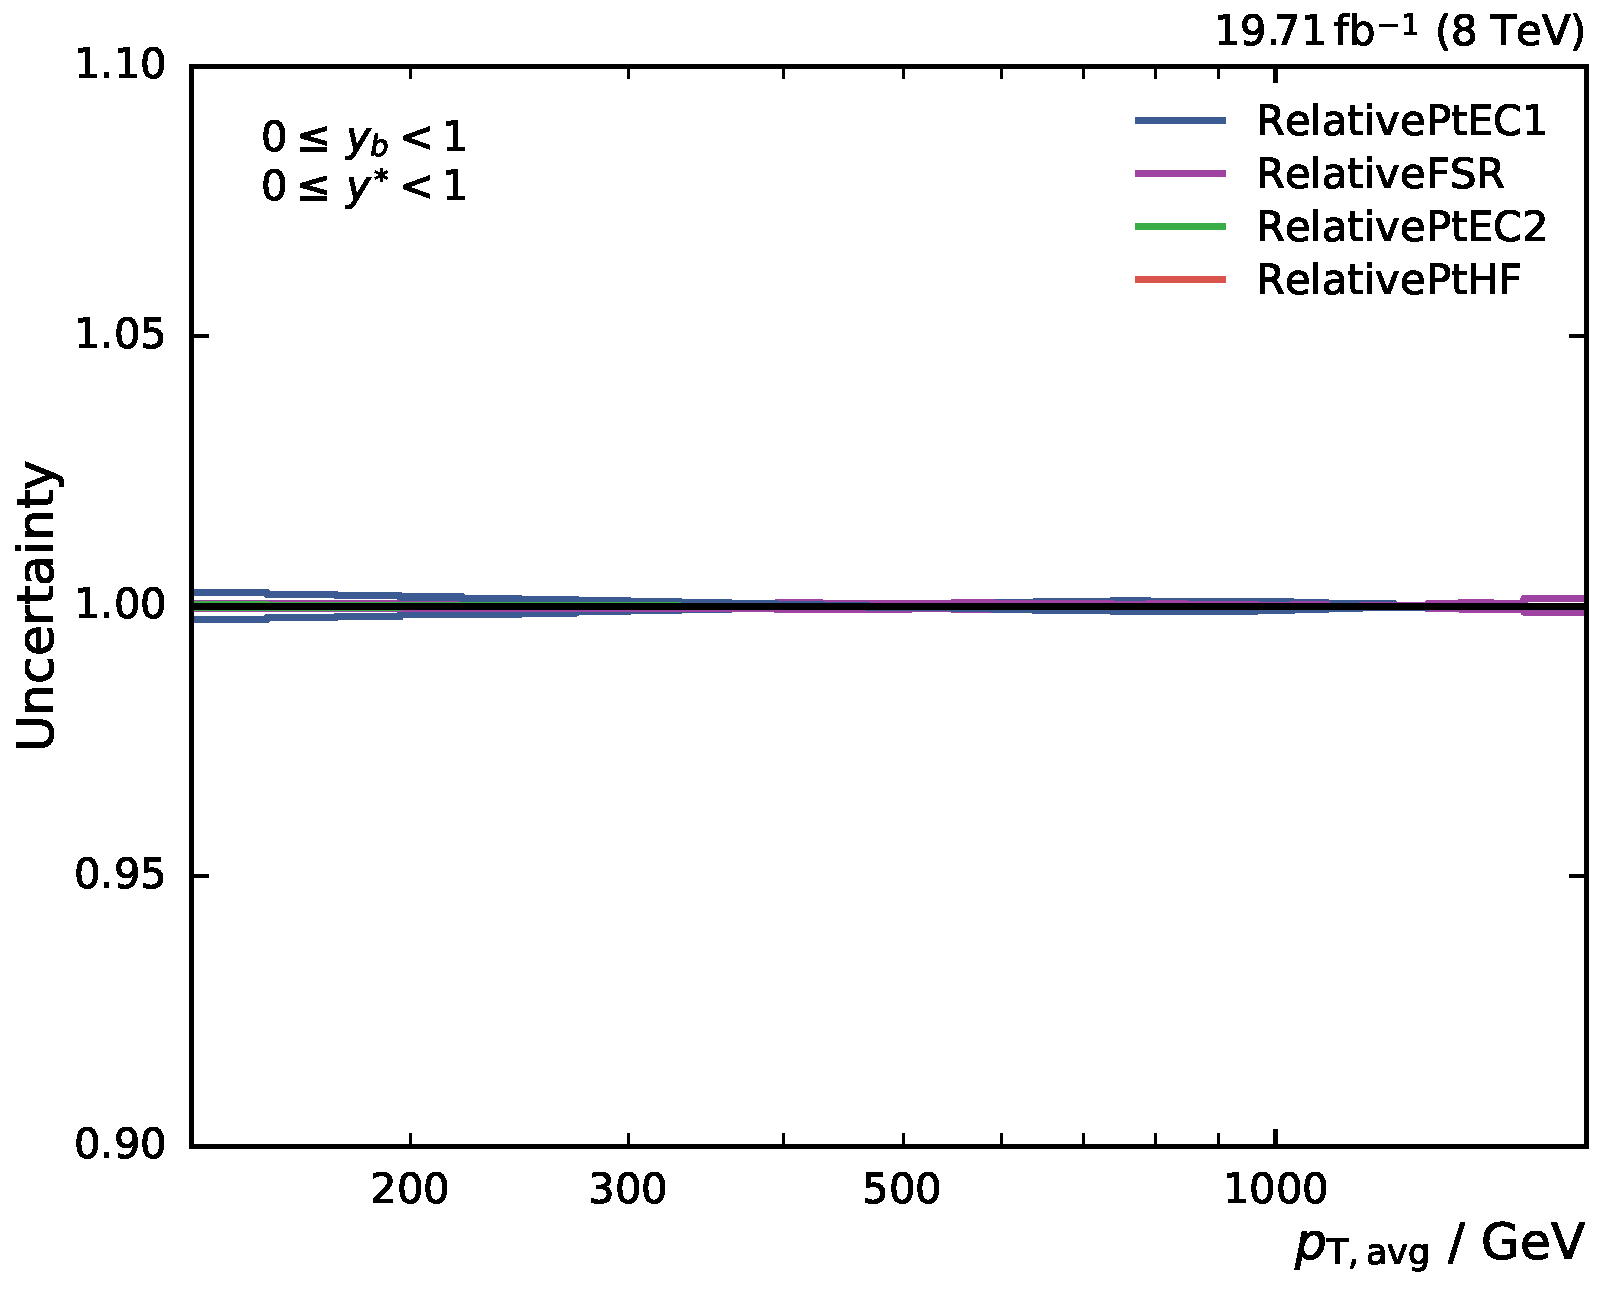
\includegraphics[width=0.49\textwidth]{figures/measurement/jec_relunc_3_yb0ys0.pdf}\hfill
    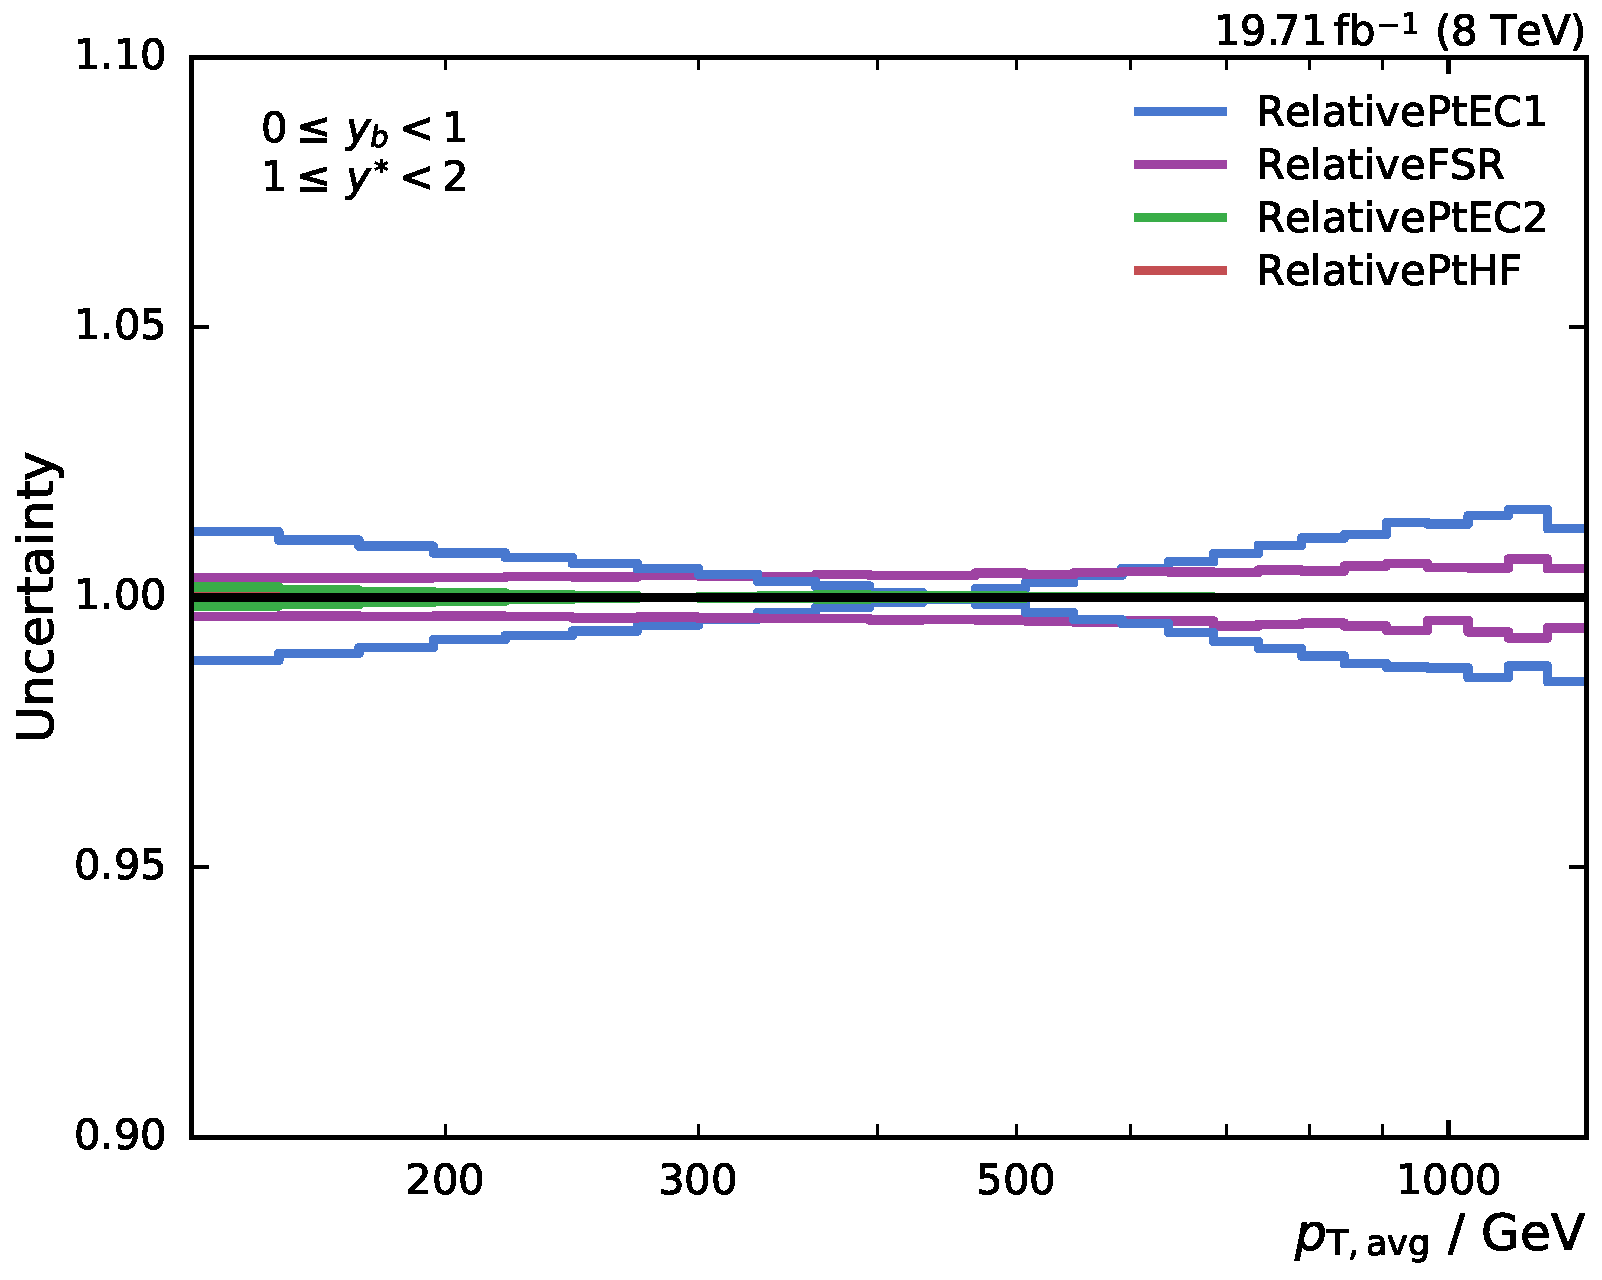
\includegraphics[width=0.49\textwidth]{figures/measurement/jec_relunc_3_yb0ys1.pdf}
    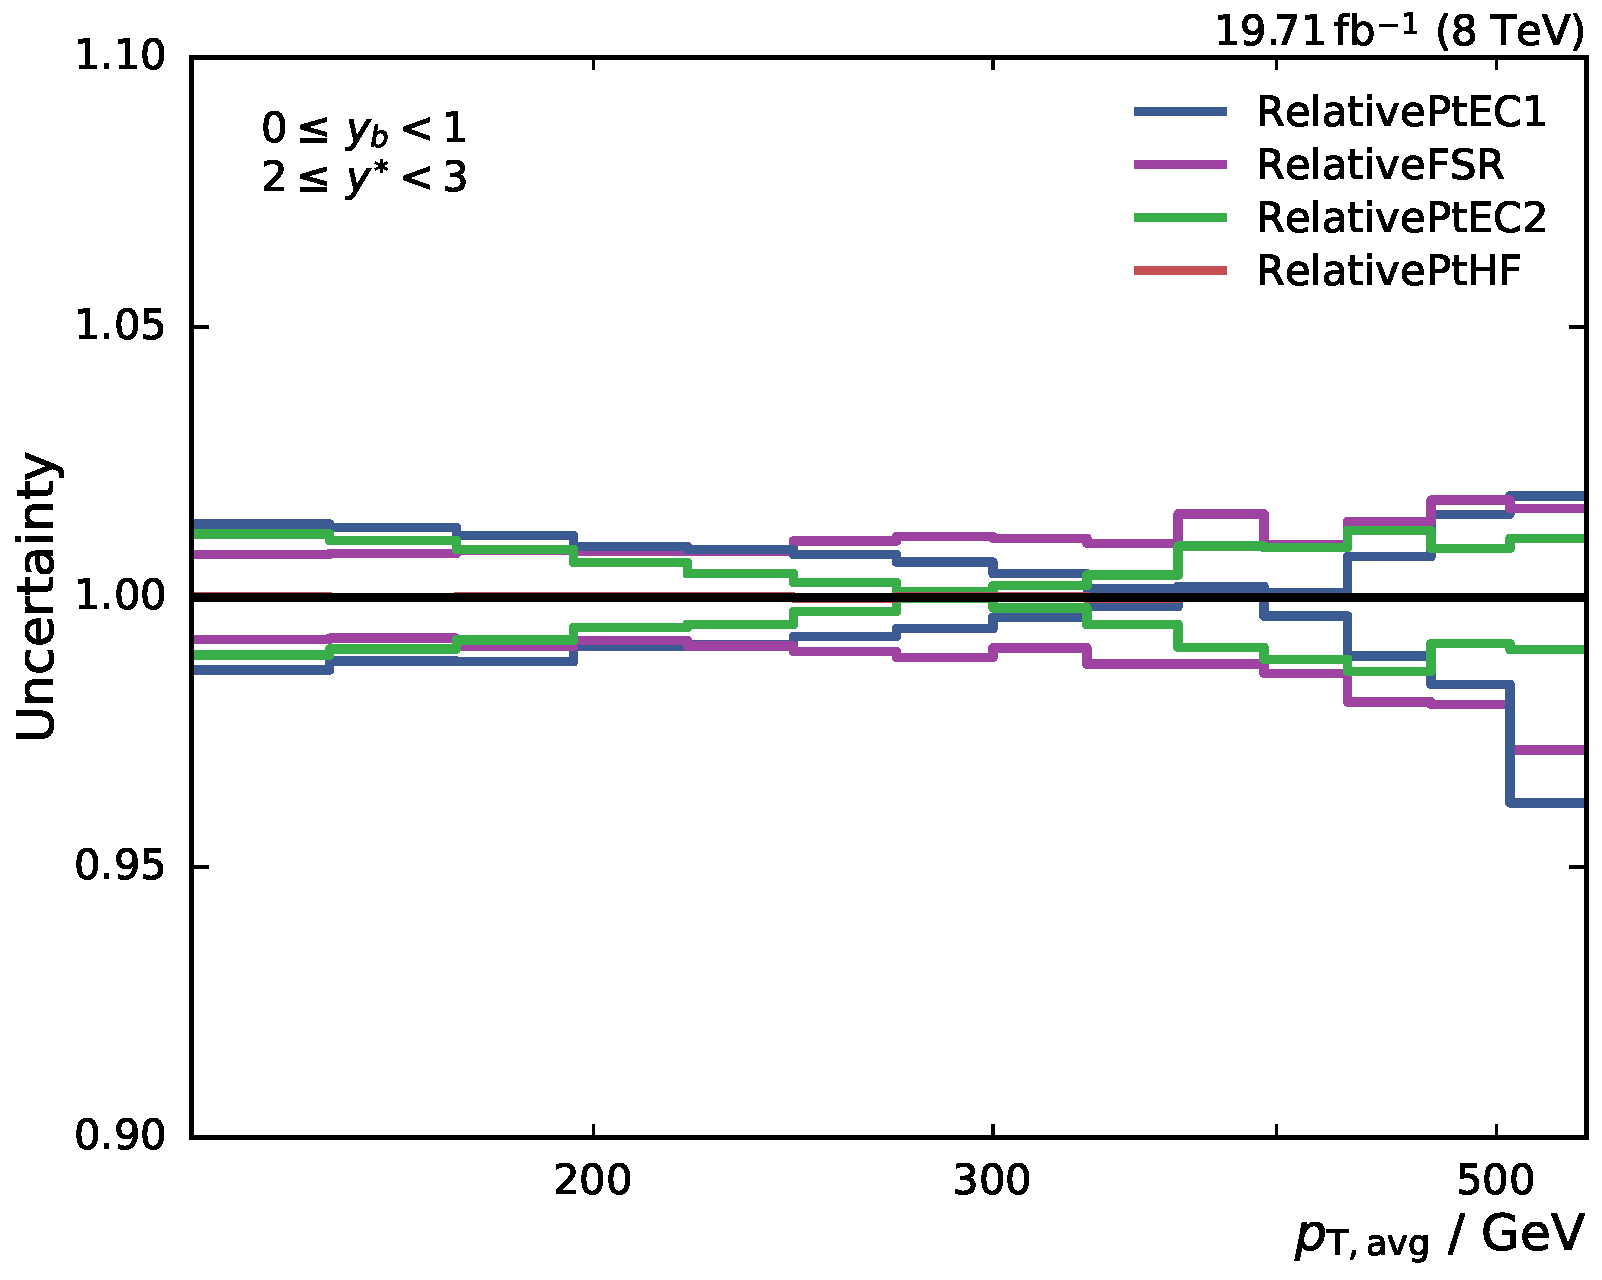
\includegraphics[width=0.49\textwidth]{figures/measurement/jec_relunc_3_yb0ys2.pdf}\hfill
    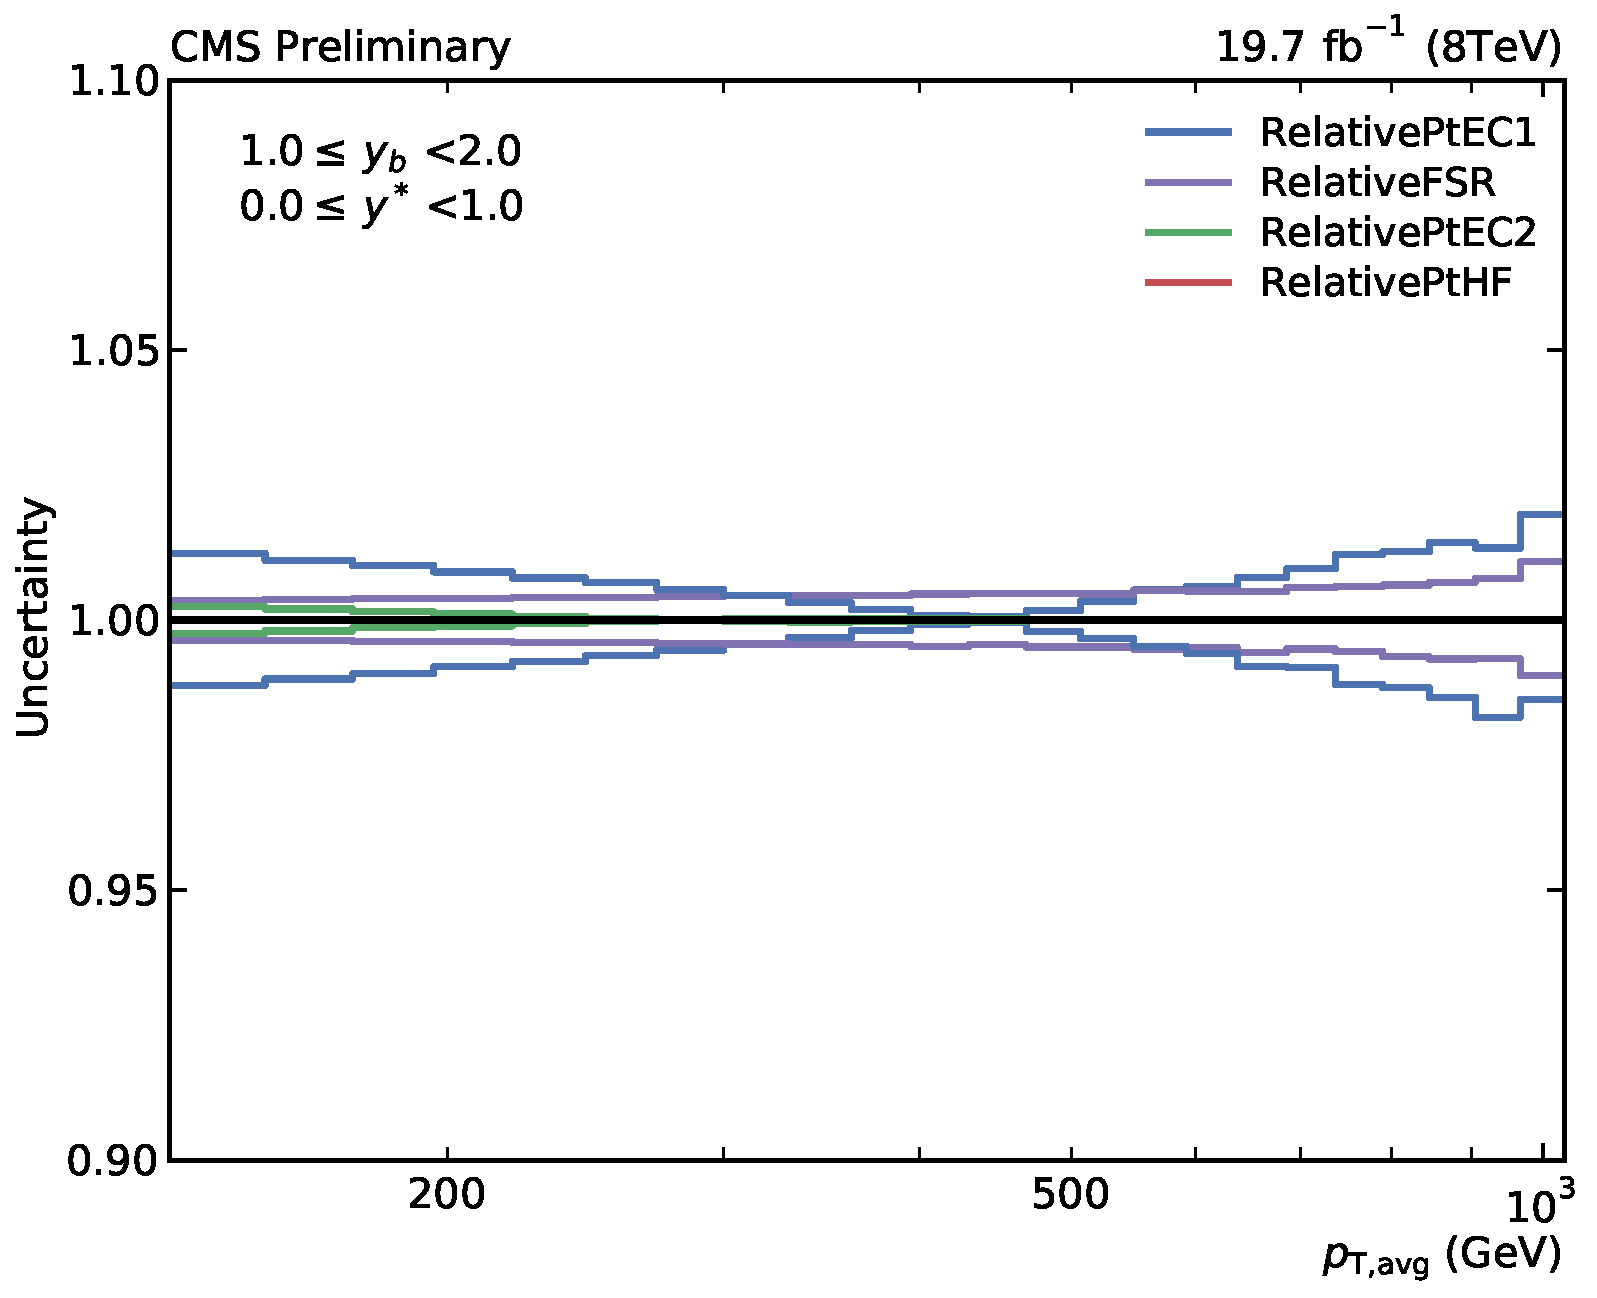
\includegraphics[width=0.49\textwidth]{figures/measurement/jec_relunc_3_yb1ys0.pdf}
    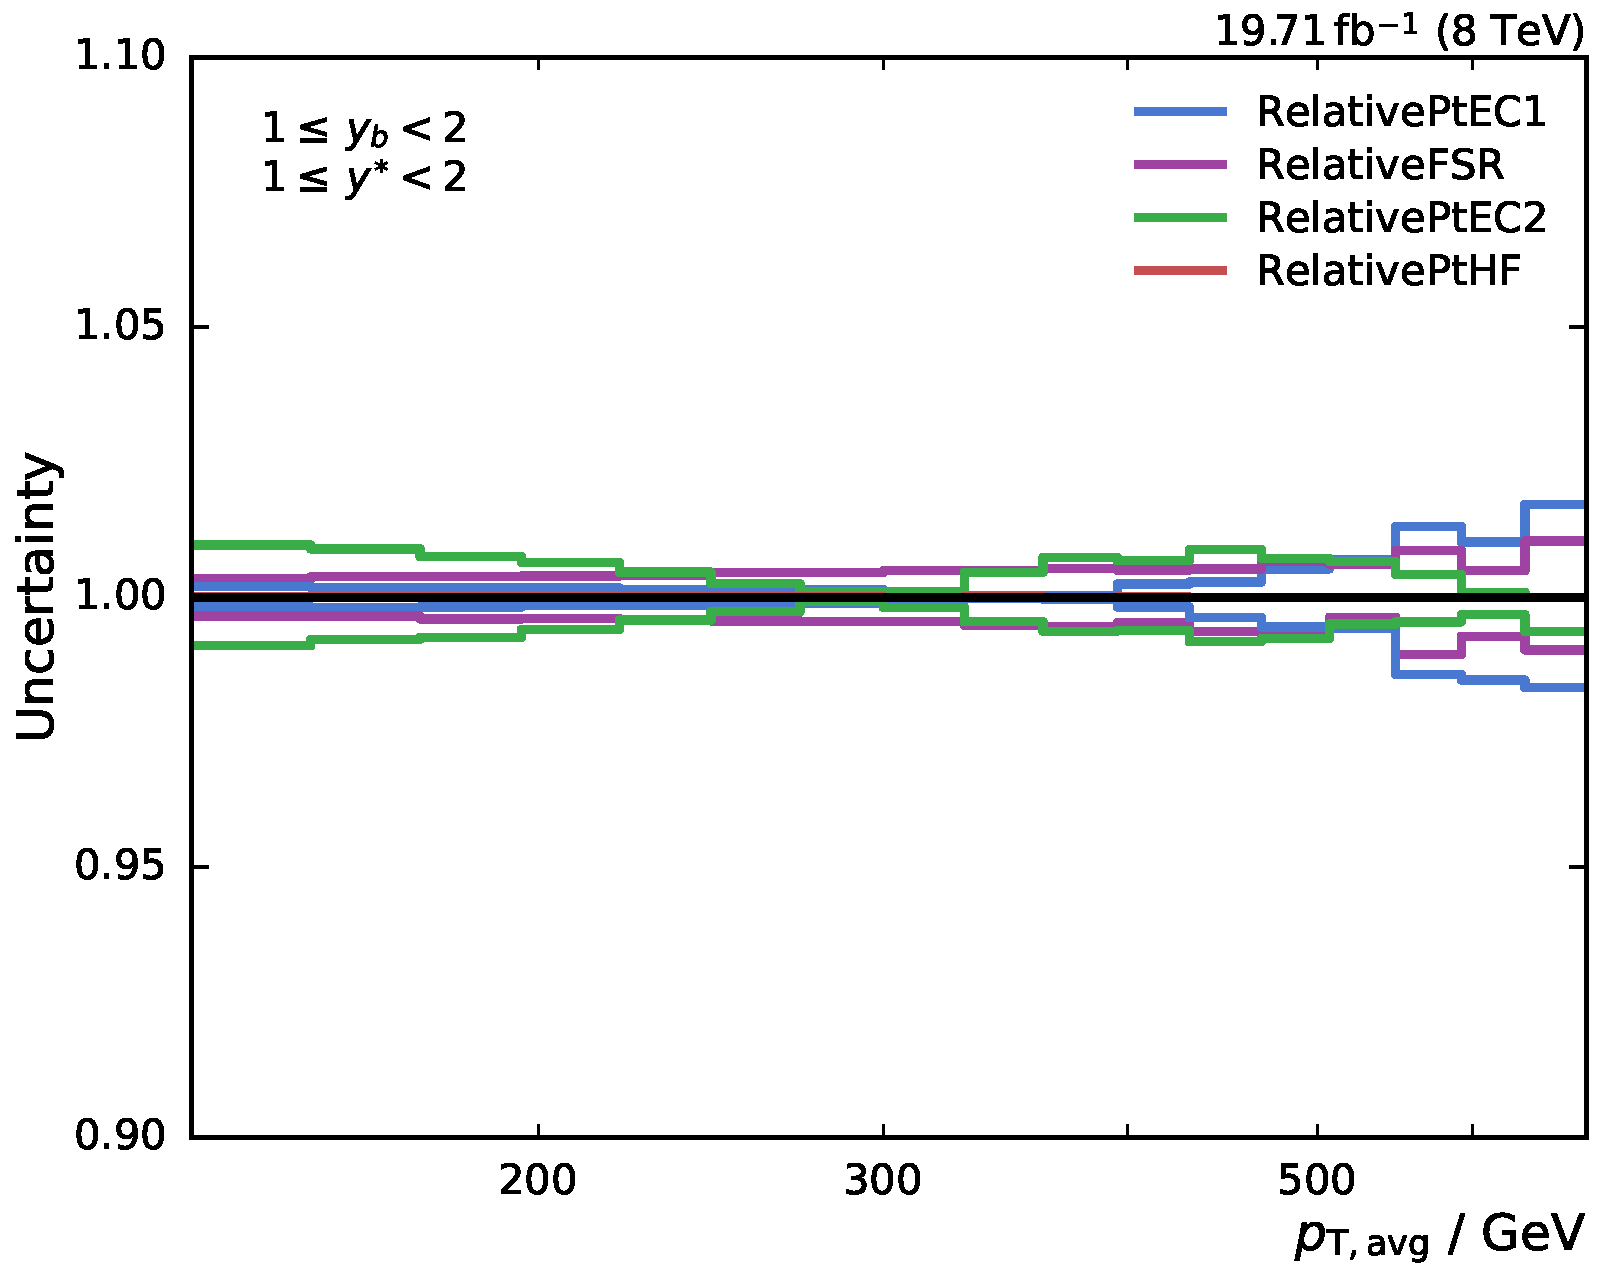
\includegraphics[width=0.49\textwidth]{figures/measurement/jec_relunc_3_yb1ys1.pdf}\hfill
    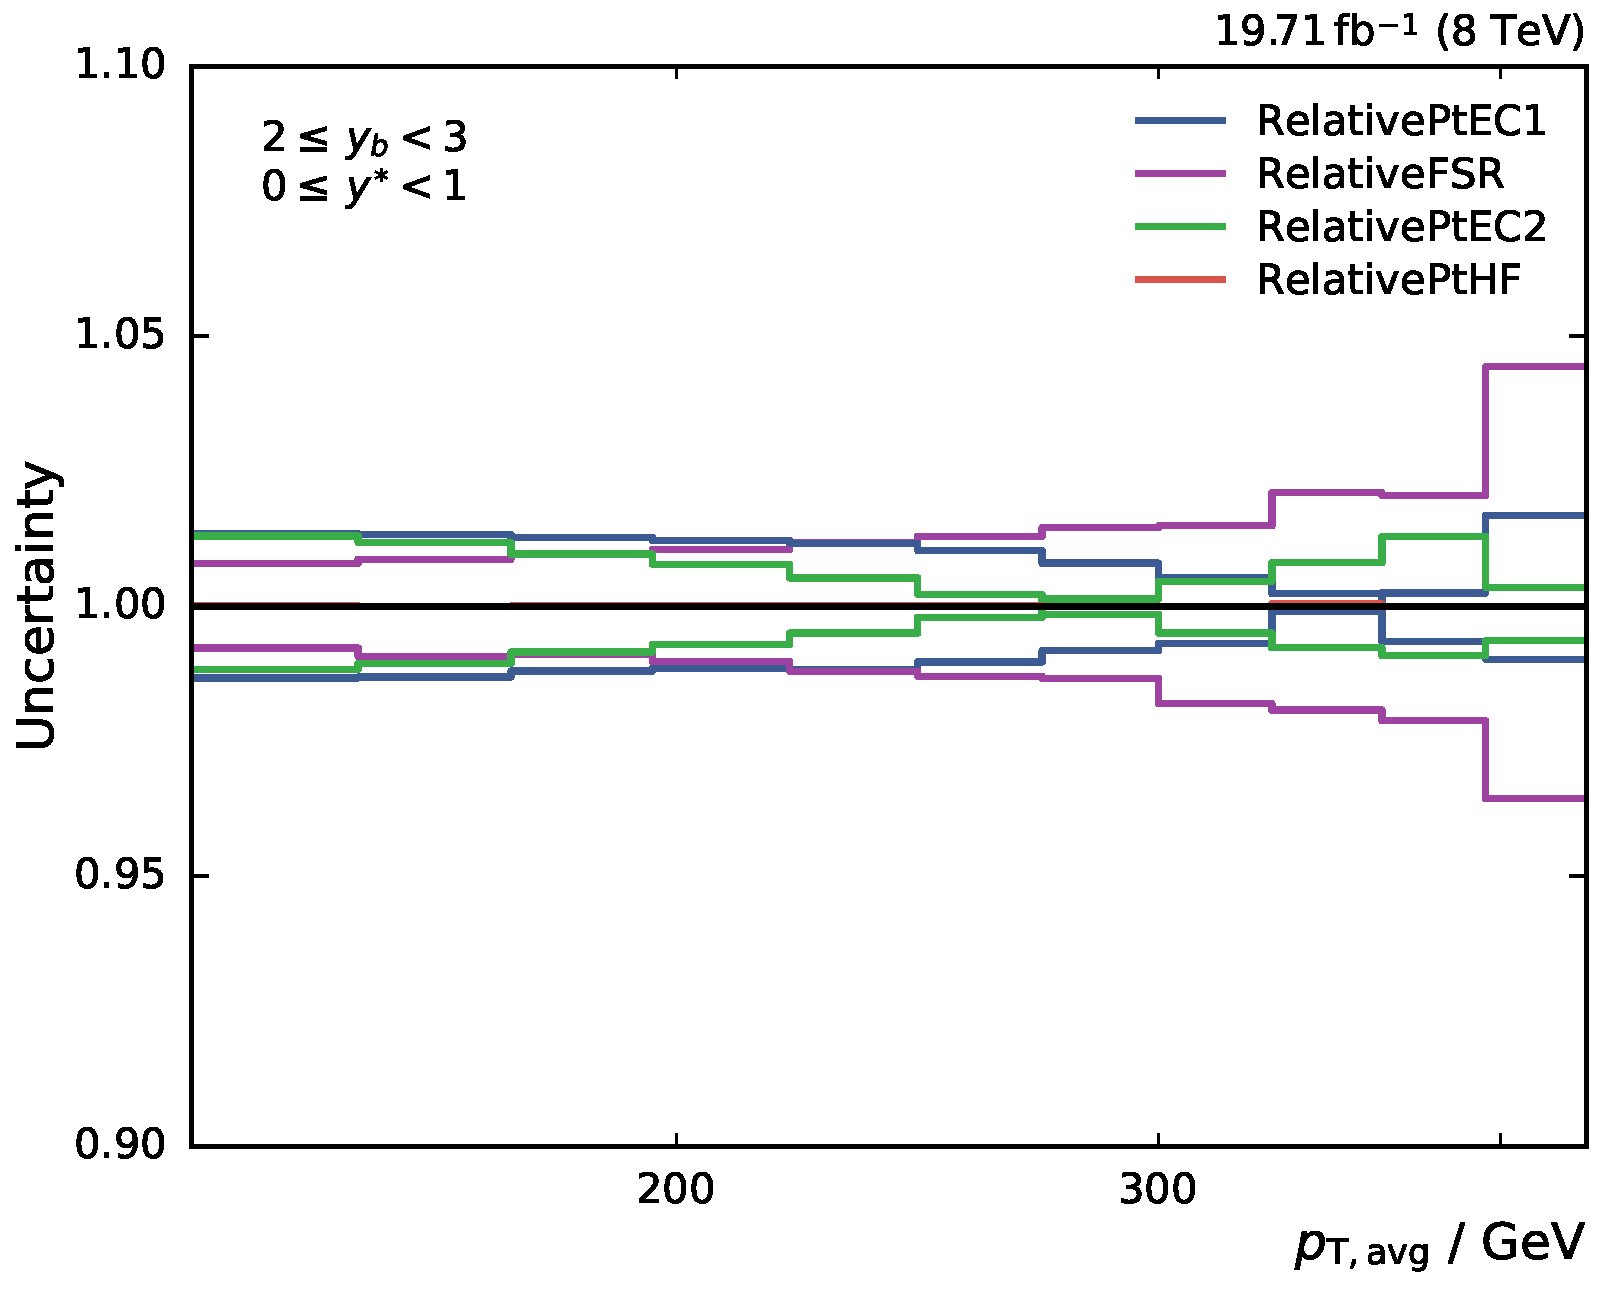
\includegraphics[width=0.49\textwidth]{figures/measurement/jec_relunc_3_yb2ys0.pdf}
    \caption[Split-up of JEC uncertainty sources: Part IV] {The relative size of the jet energy scale
             uncertainties for the sources RelativePtEC1, RelativePtEC2,
             RelativeFSR, and RelativePtHF are shown for all \ystar and \yboost bins.}

    \label{fig:jec_relunc_3}
\end{figure}

\begin{figure}[htbp]
    \centering
    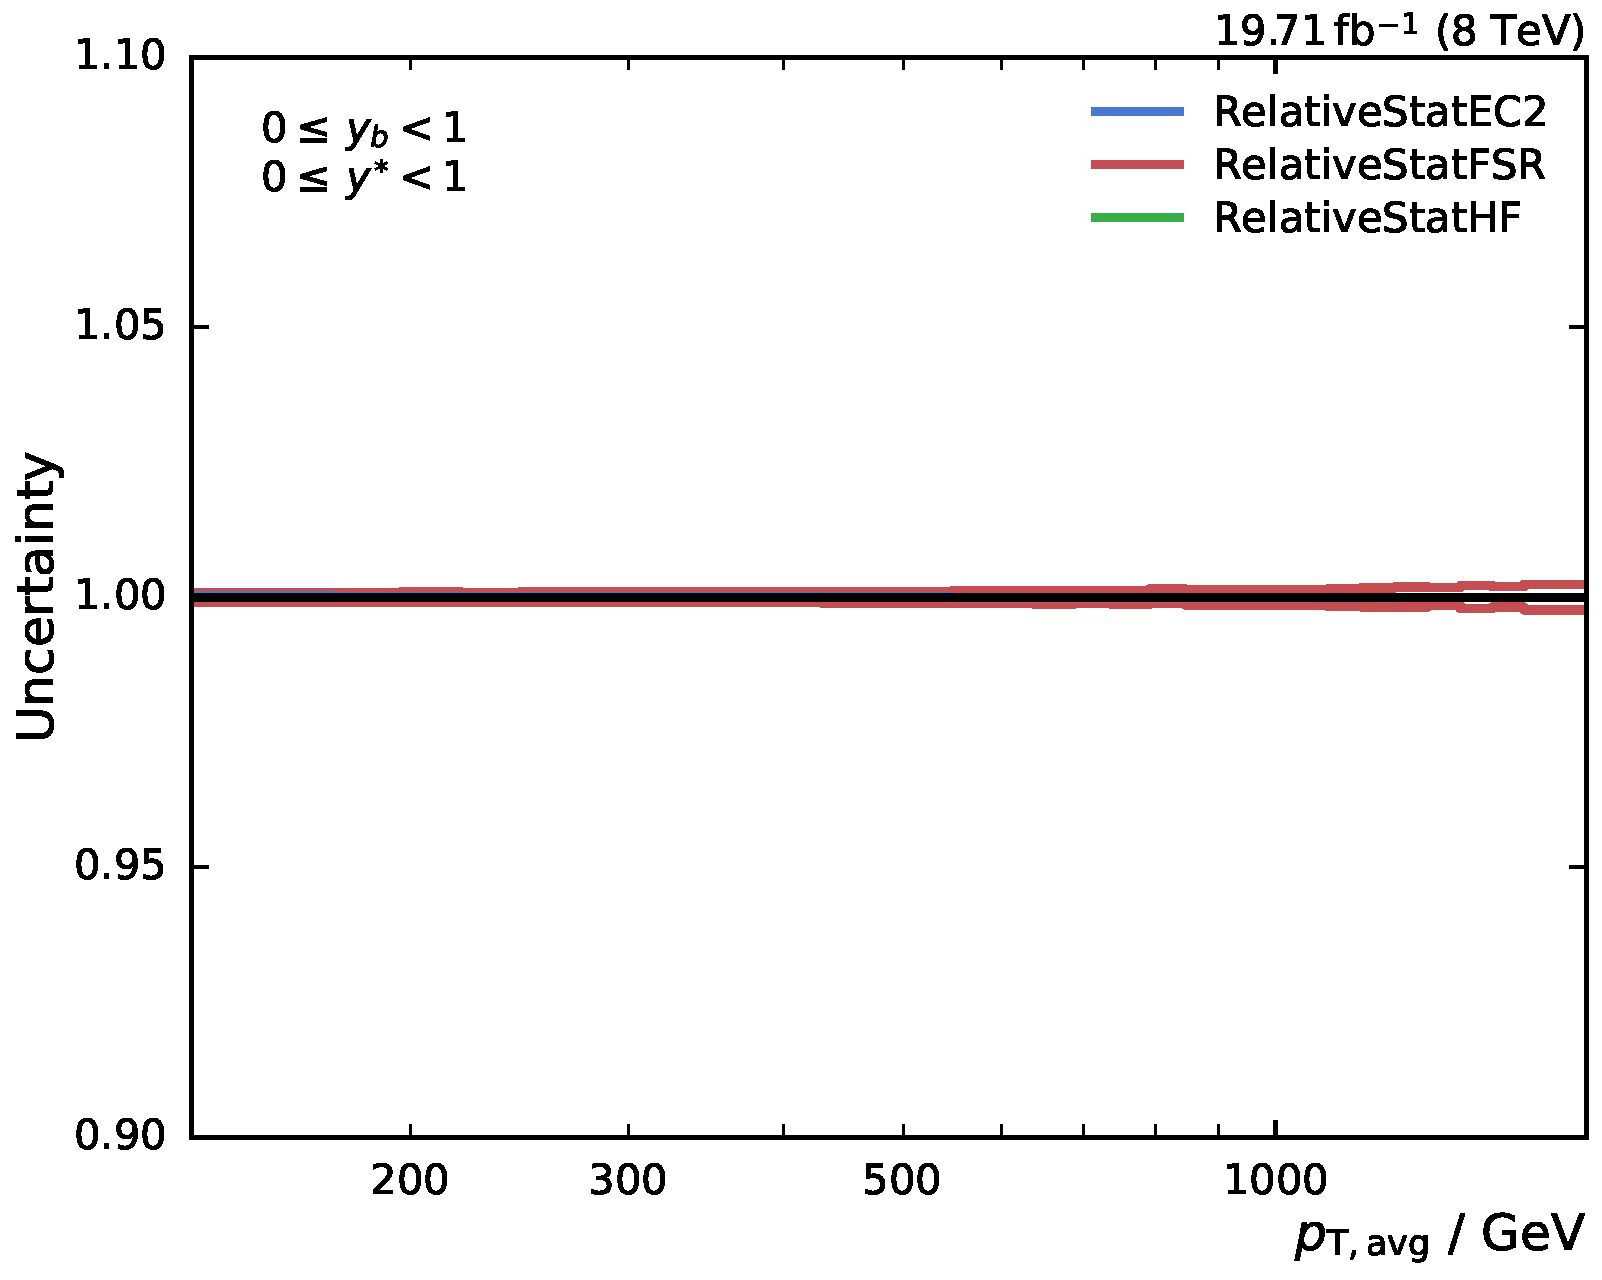
\includegraphics[width=0.49\textwidth]{figures/measurement/jec_relunc_4_yb0ys0.pdf}\hfill
    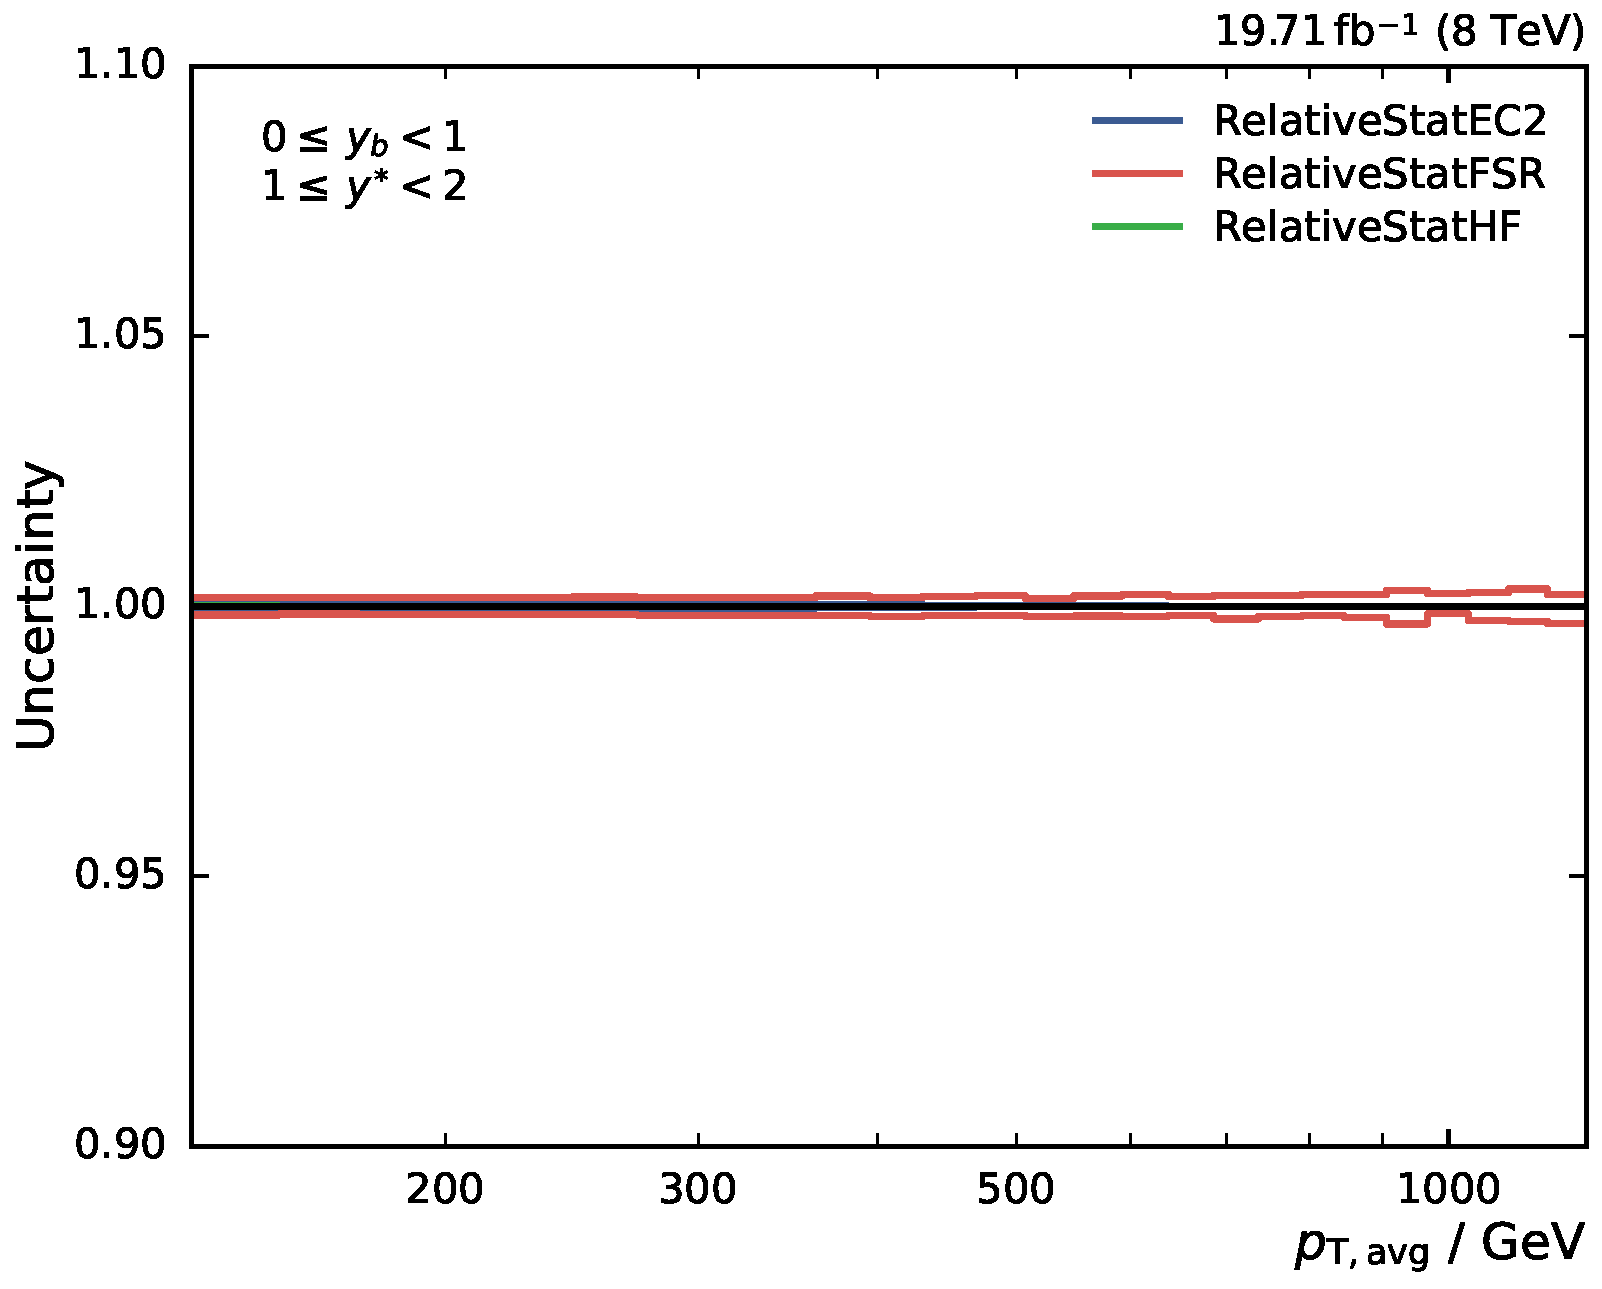
\includegraphics[width=0.49\textwidth]{figures/measurement/jec_relunc_4_yb0ys1.pdf}
    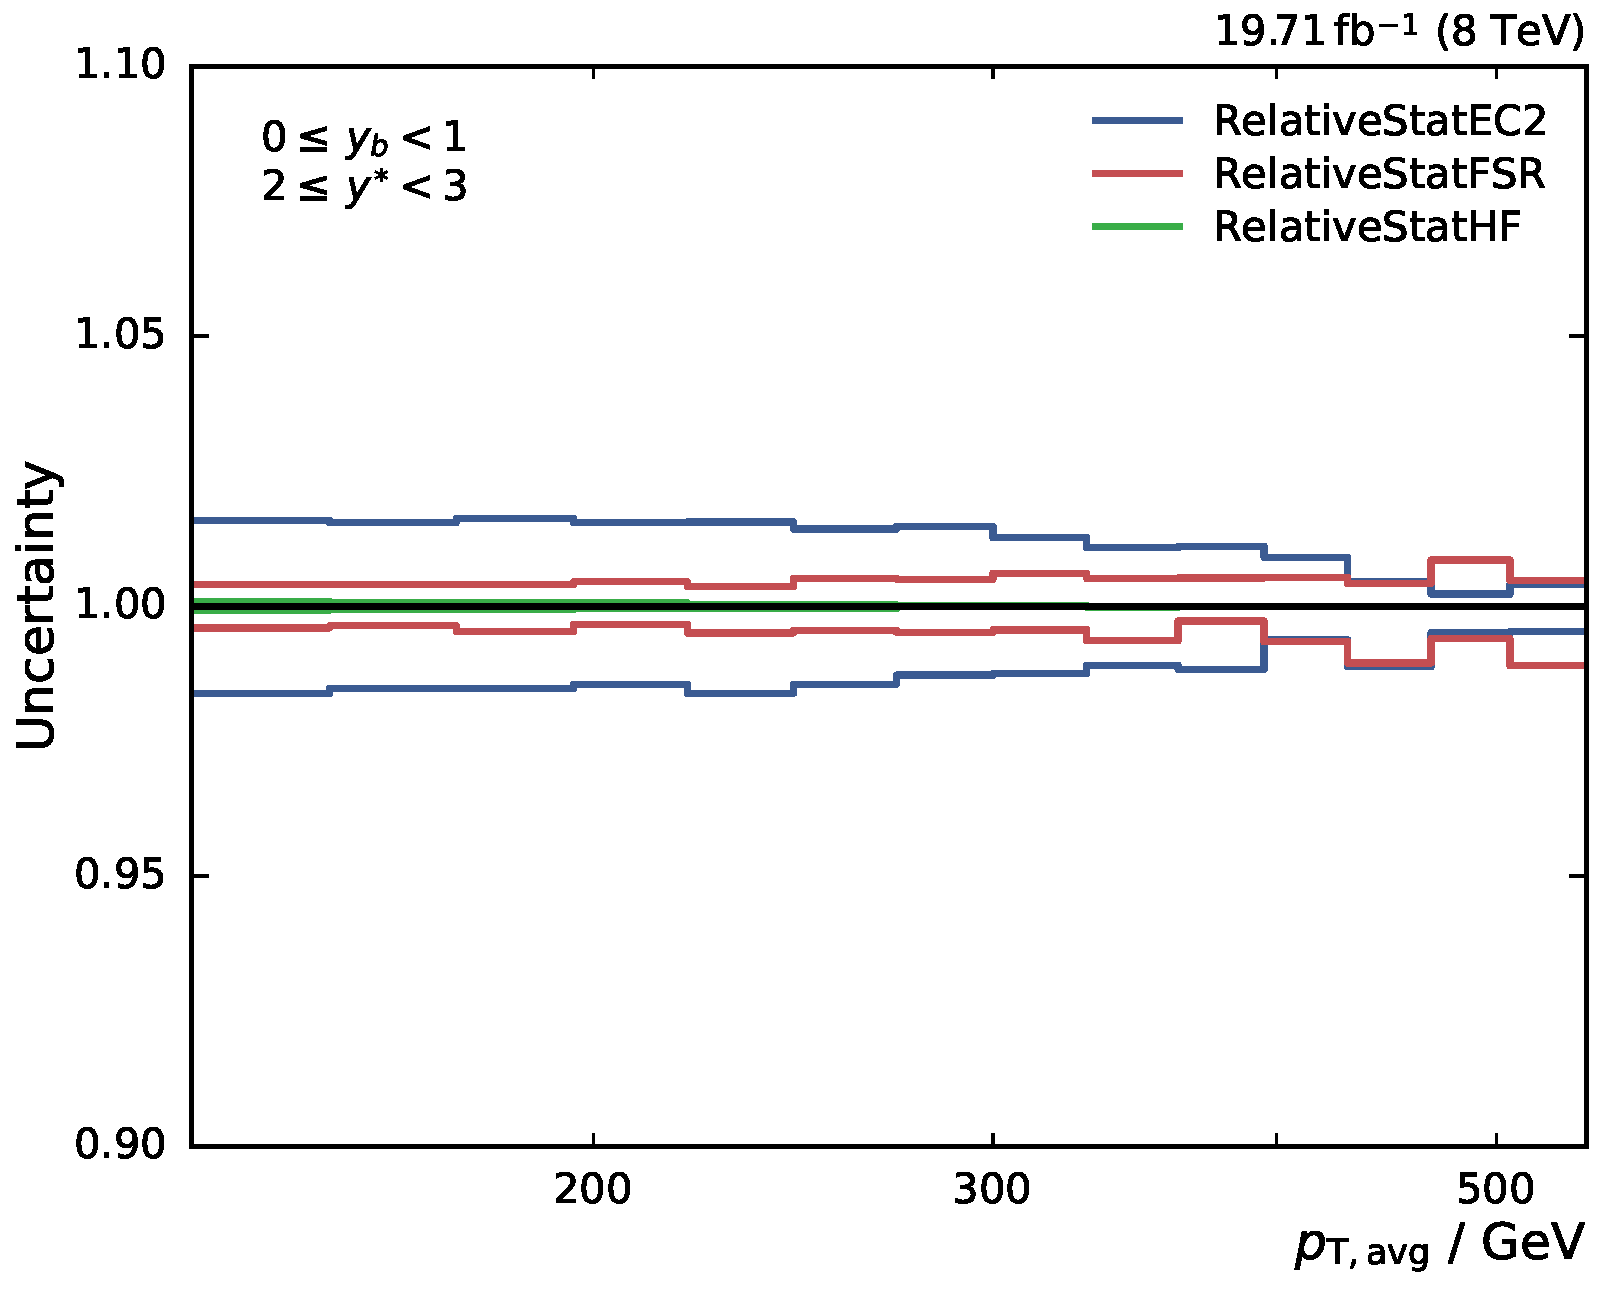
\includegraphics[width=0.49\textwidth]{figures/measurement/jec_relunc_4_yb0ys2.pdf}\hfill
    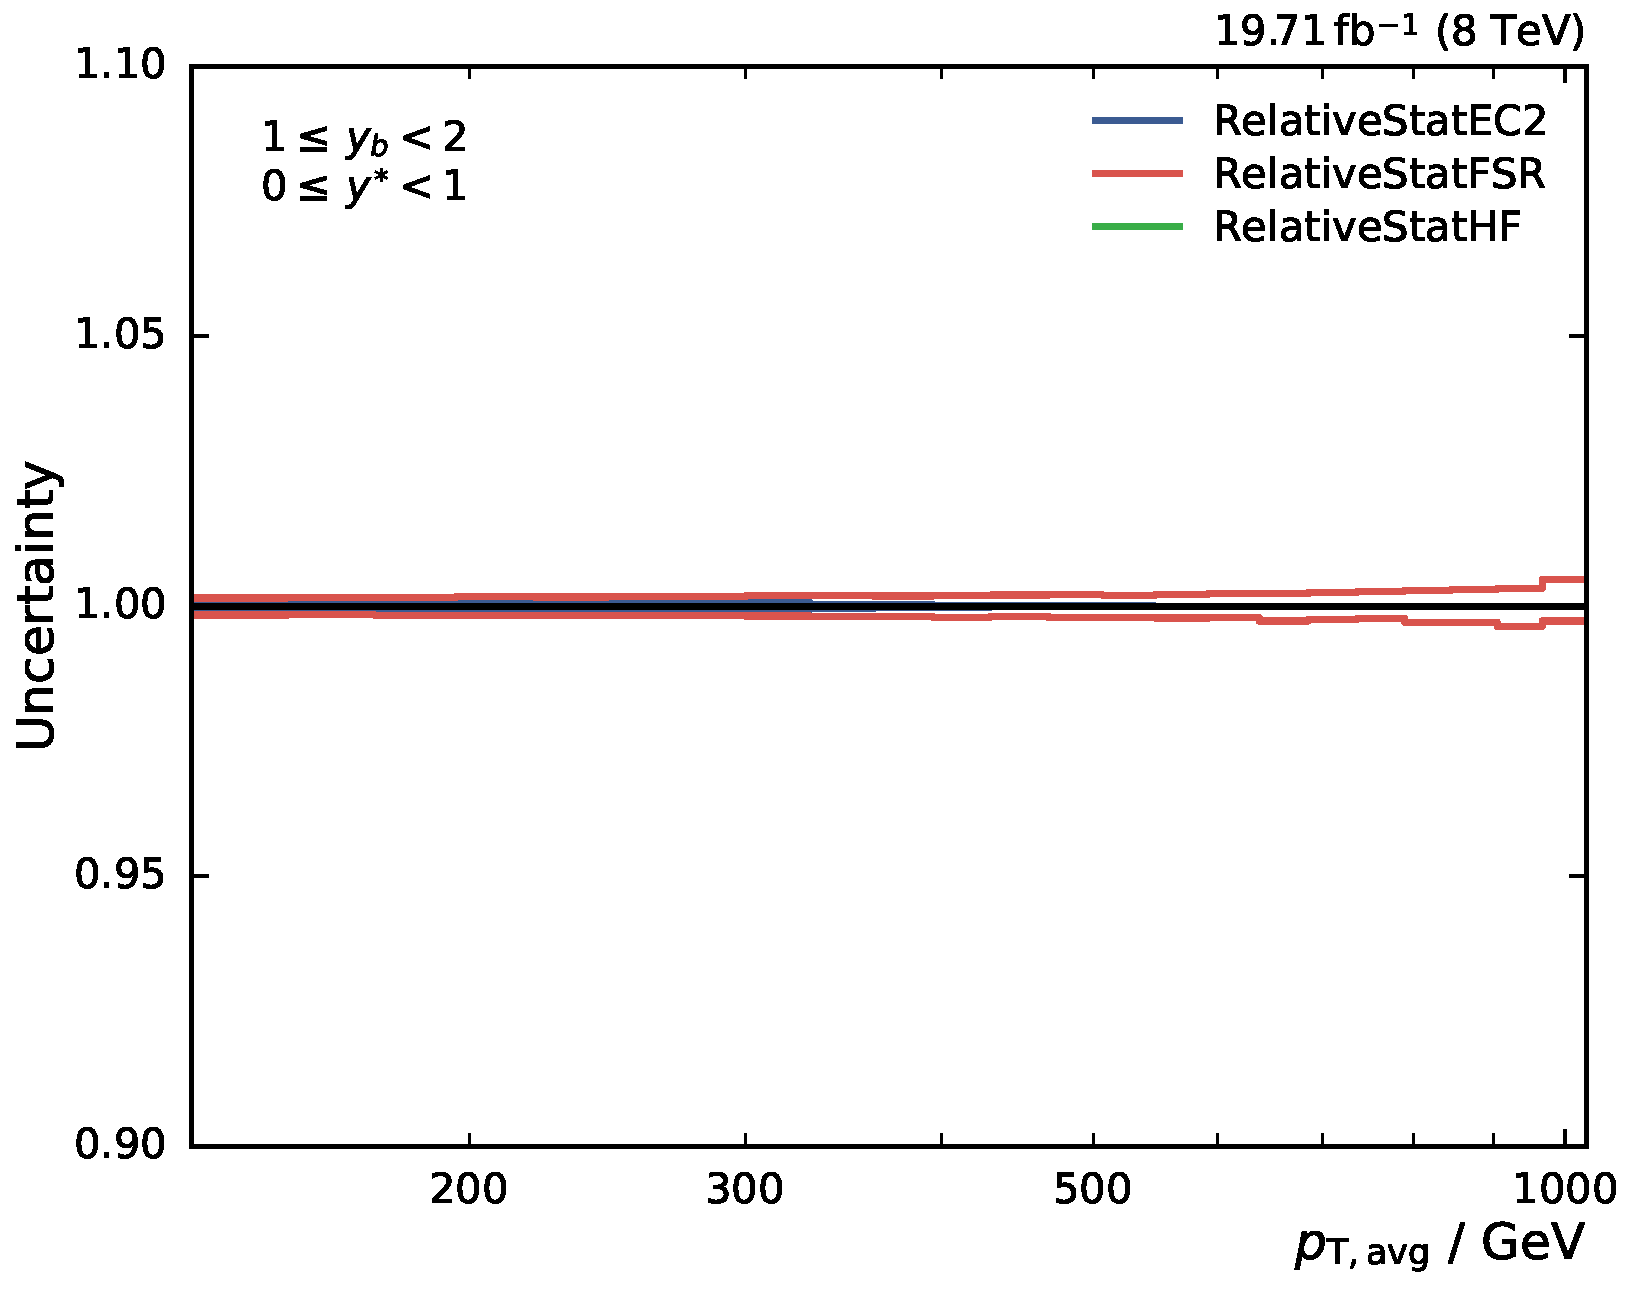
\includegraphics[width=0.49\textwidth]{figures/measurement/jec_relunc_4_yb1ys0.pdf}
    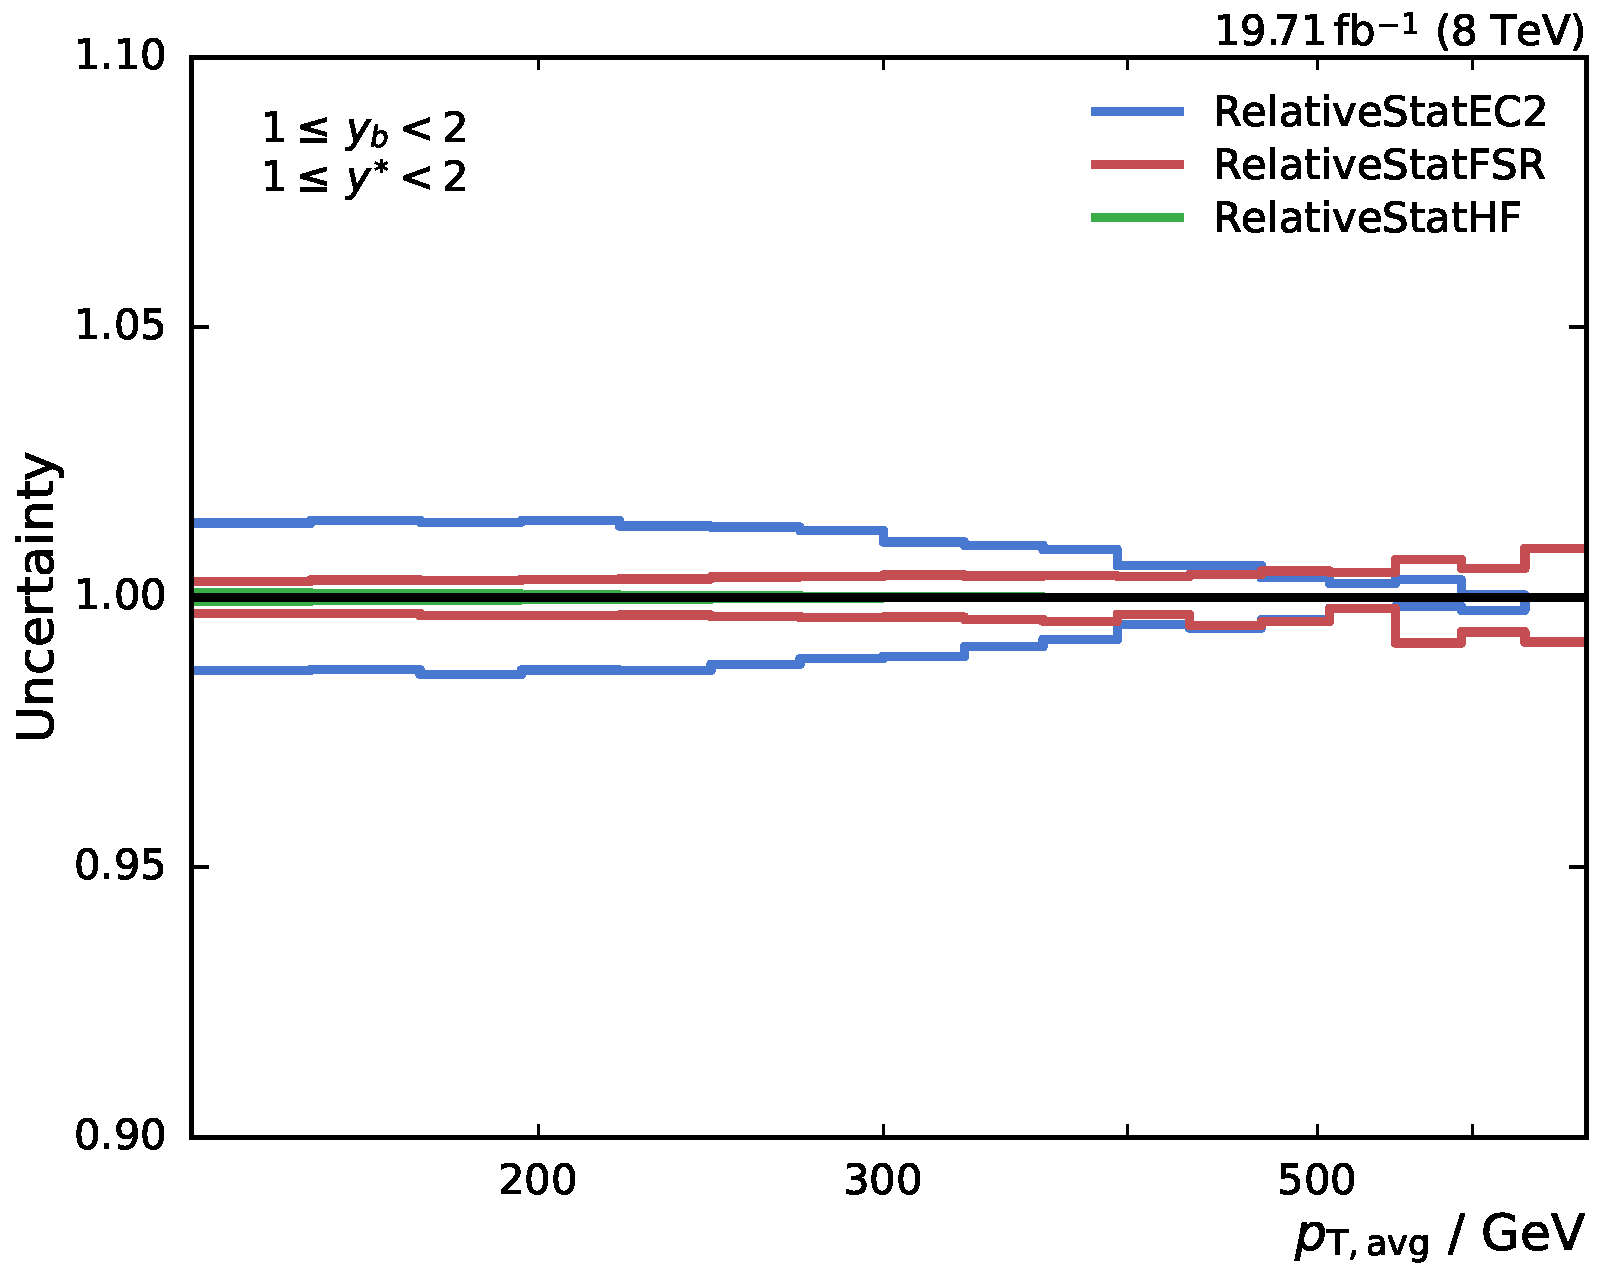
\includegraphics[width=0.49\textwidth]{figures/measurement/jec_relunc_4_yb1ys1.pdf}\hfill
    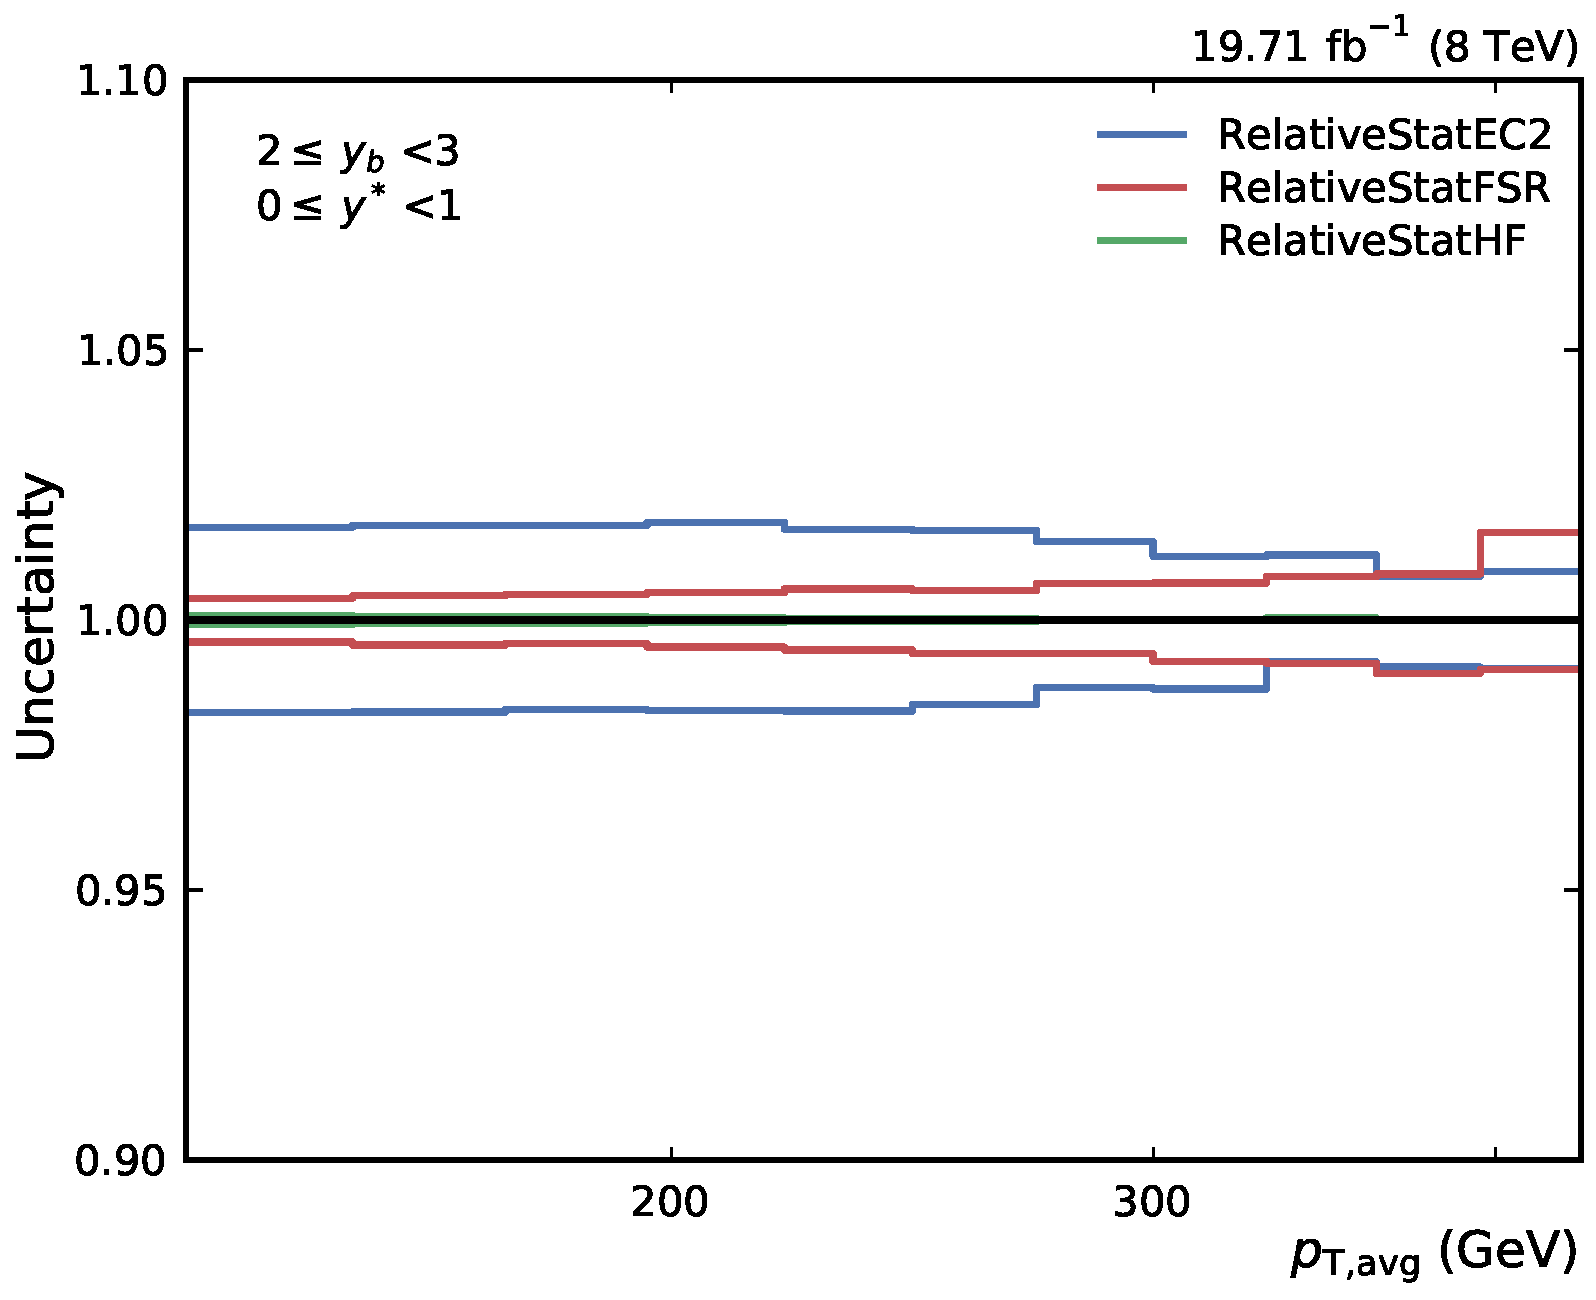
\includegraphics[width=0.49\textwidth]{figures/measurement/jec_relunc_4_yb2ys0.pdf}
    \caption[Split-up of JEC uncertainty sources: Part V]{The relative size of the jet energy scale
             uncertainties for the sources RelativeStatEC2, RelativeStatFSR, and
             RelativeStatHF are shown for all \ystar and \yboost bins.}
    \label{fig:jec_relunc_4}
\end{figure}

\begin{figure}[htbp]
    \centering
    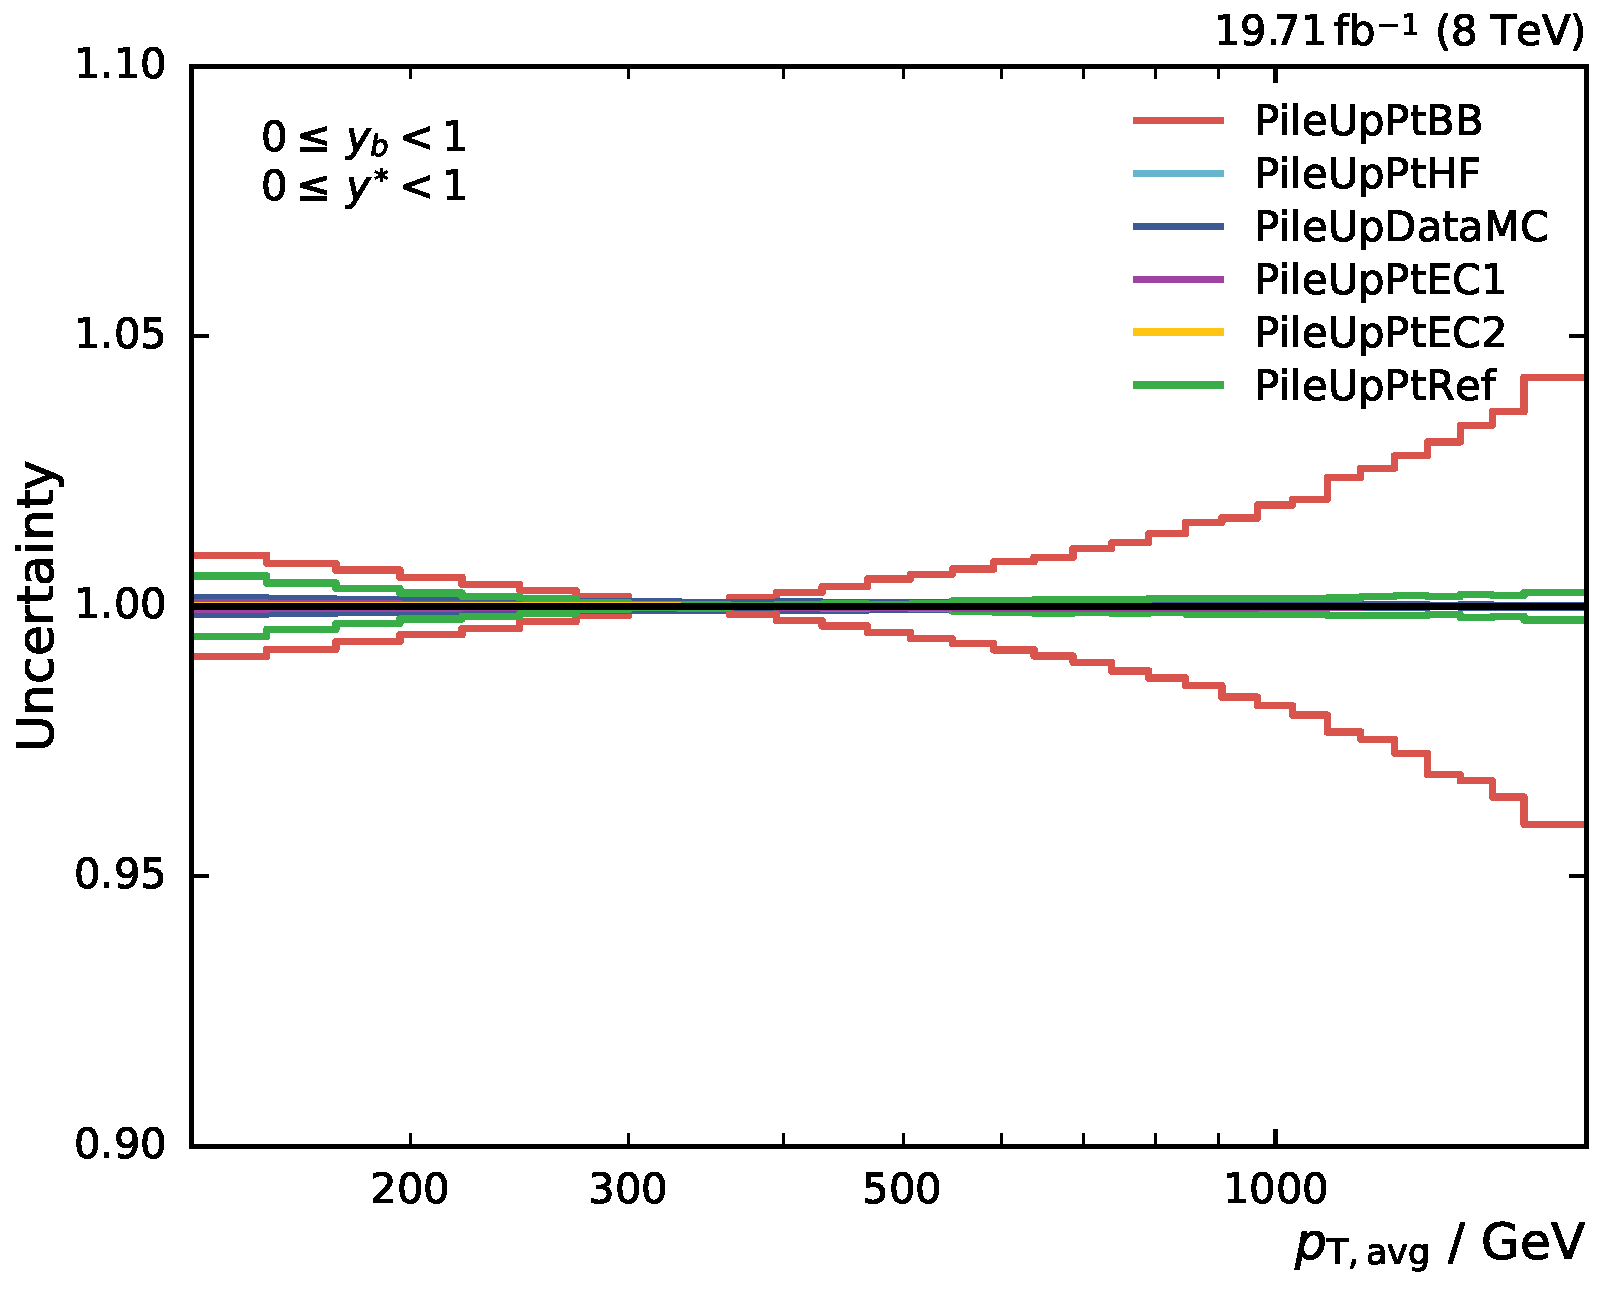
\includegraphics[width=0.49\textwidth]{figures/measurement/jec_relunc_5_yb0ys0.pdf}\hfill
    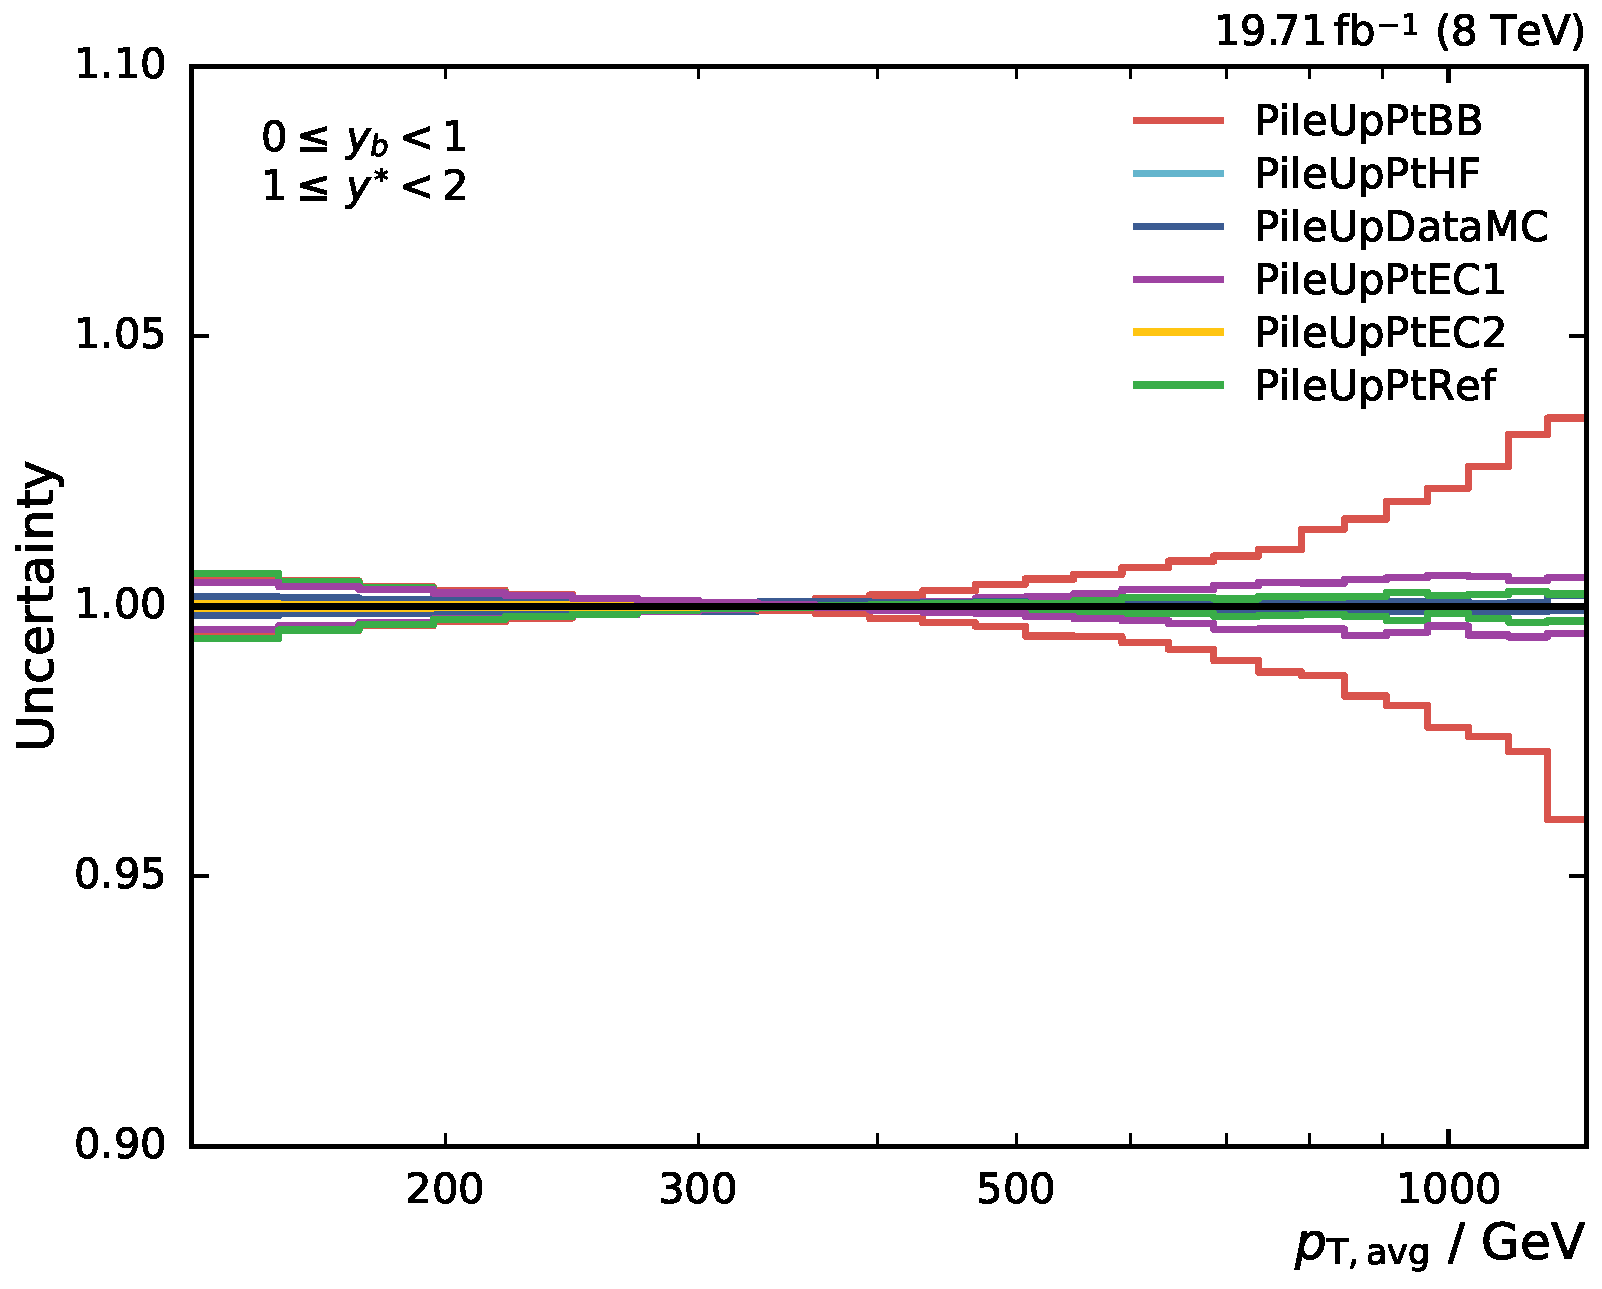
\includegraphics[width=0.49\textwidth]{figures/measurement/jec_relunc_5_yb0ys1.pdf}
    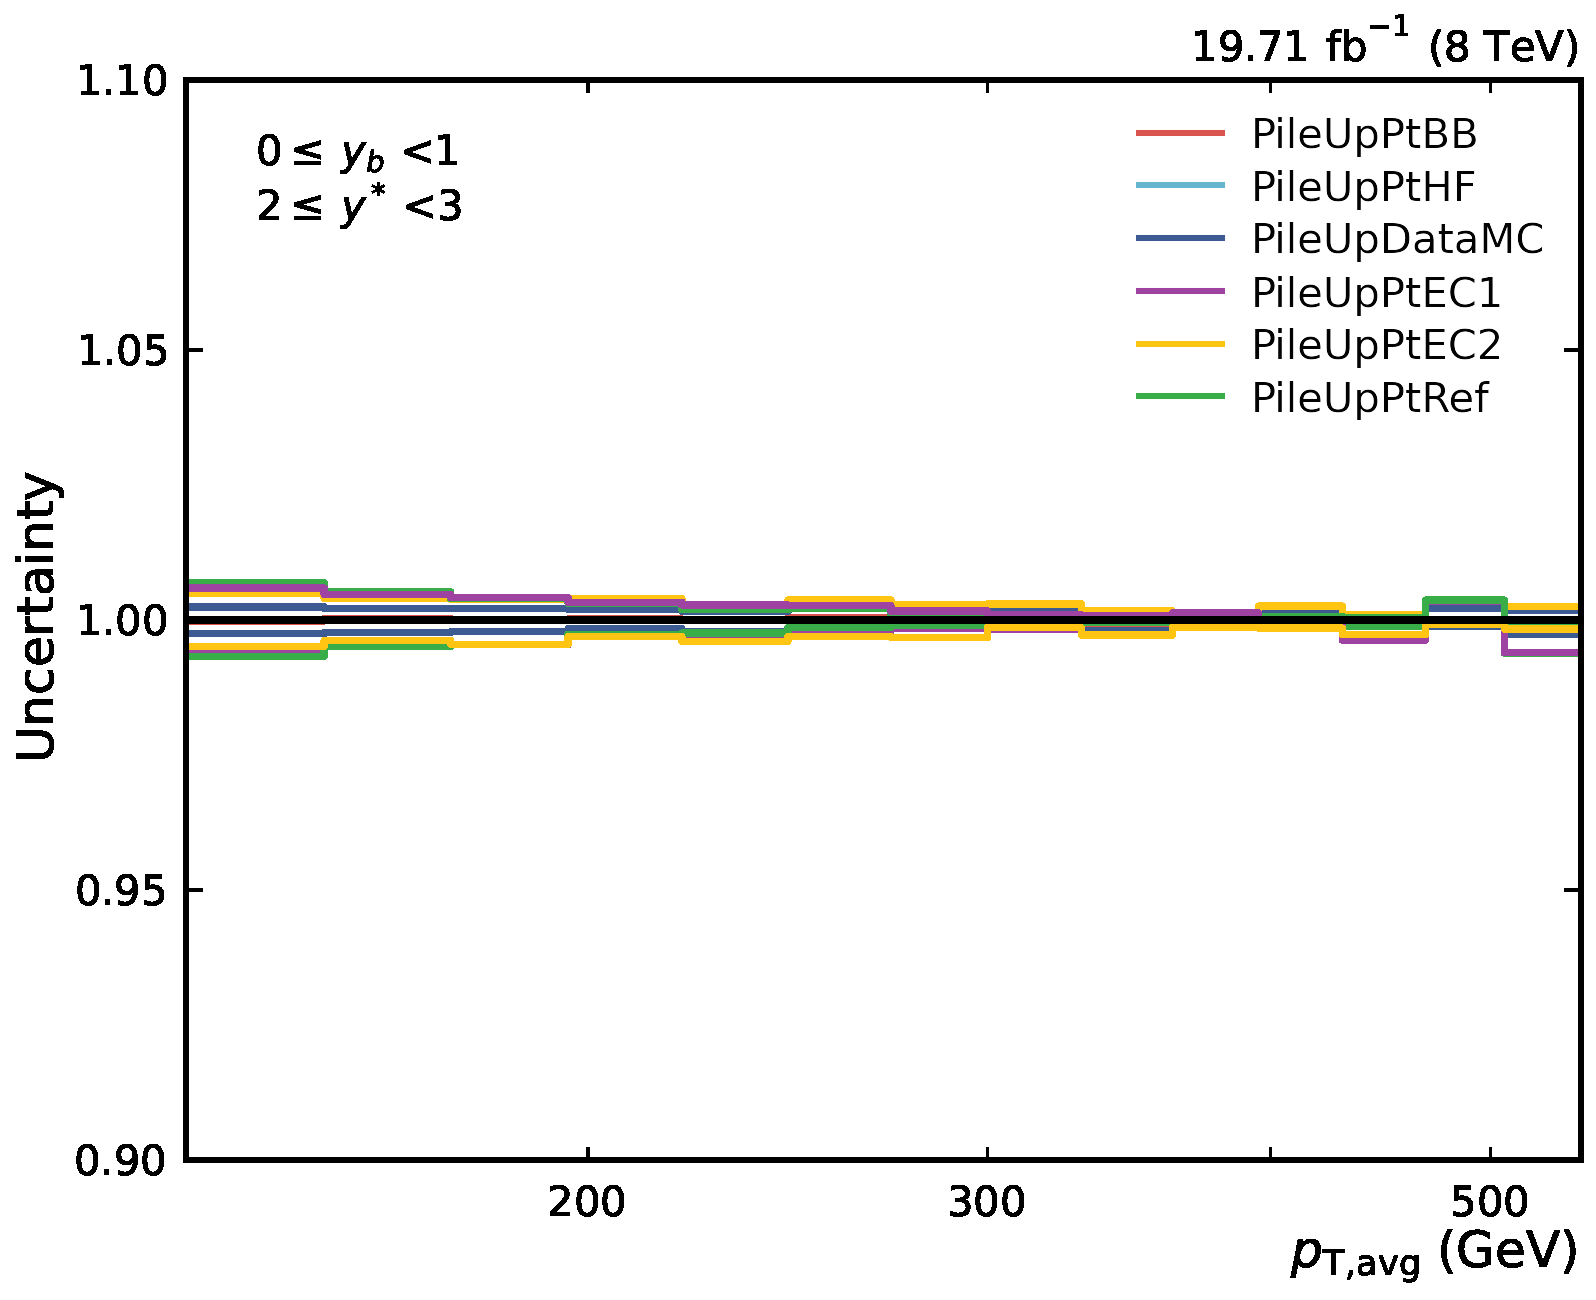
\includegraphics[width=0.49\textwidth]{figures/measurement/jec_relunc_5_yb0ys2.pdf}\hfill
    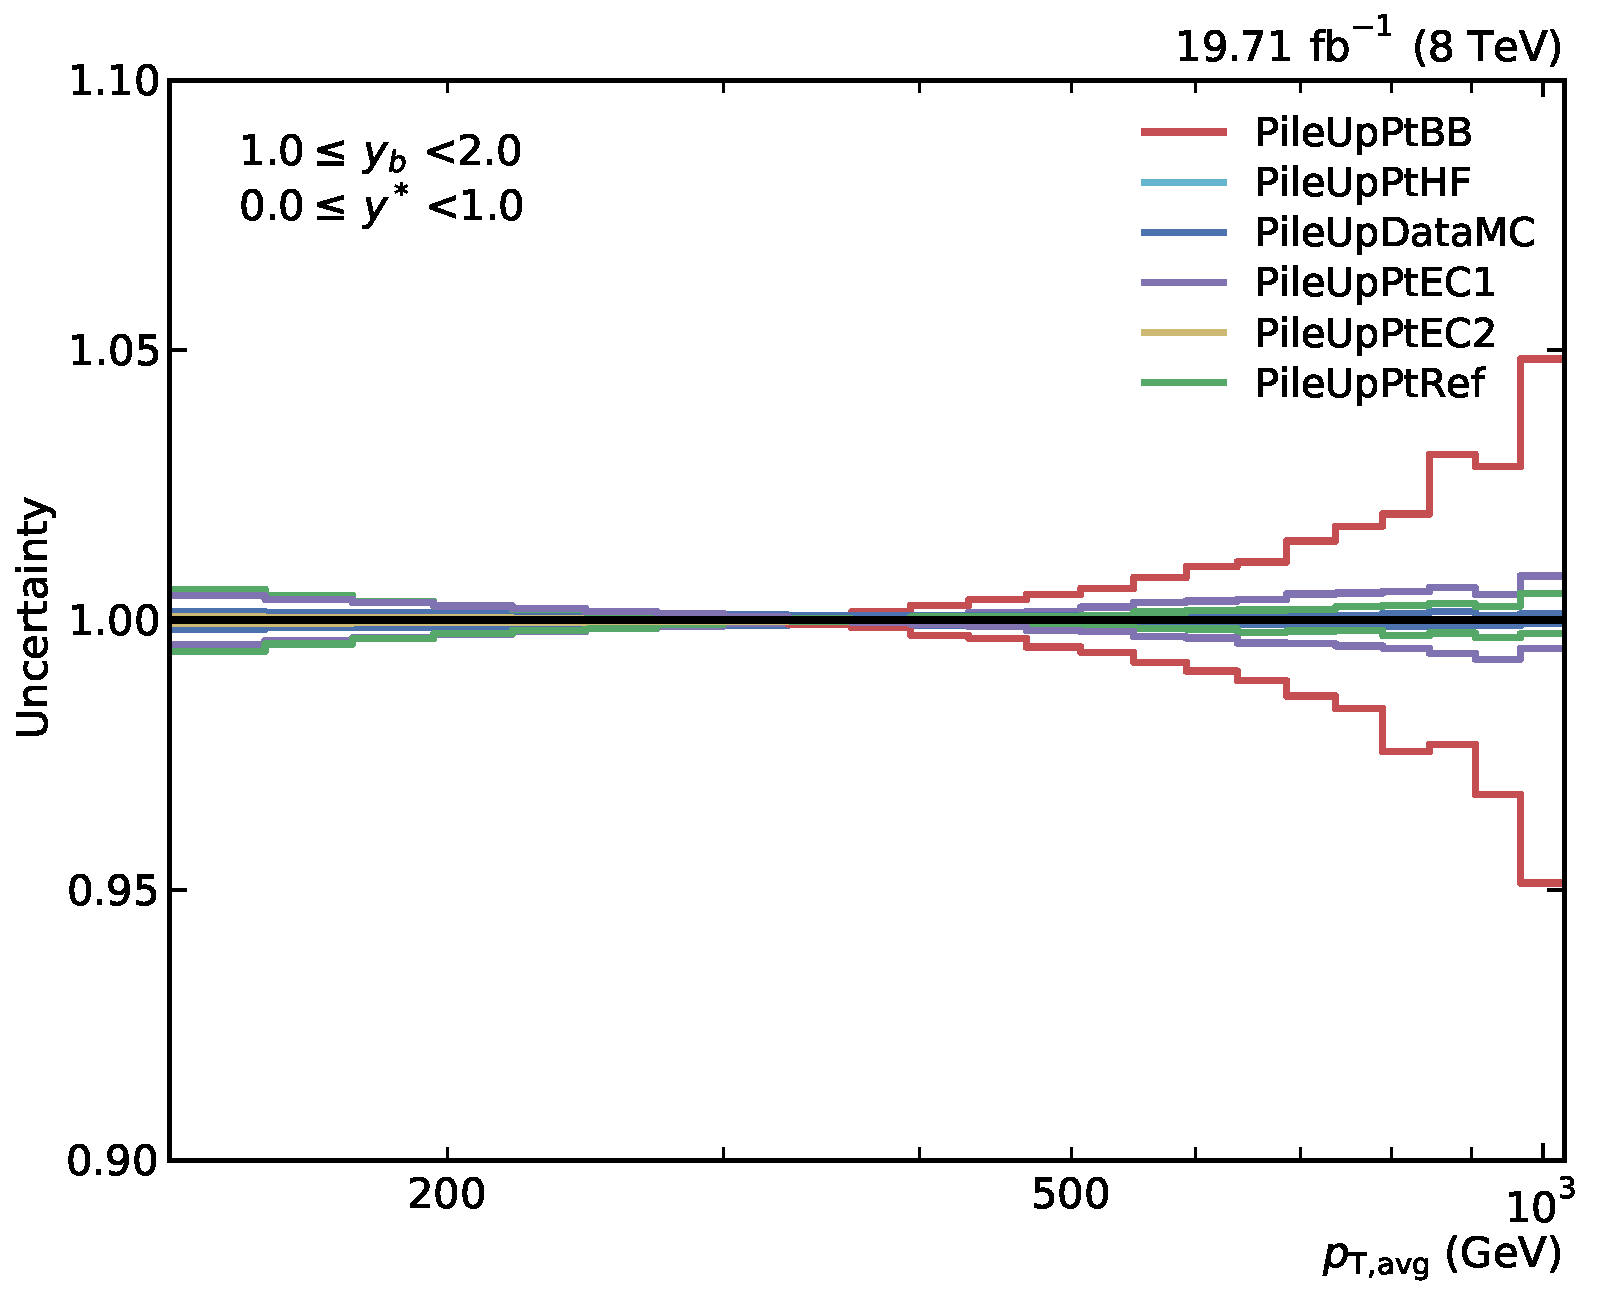
\includegraphics[width=0.49\textwidth]{figures/measurement/jec_relunc_5_yb1ys0.pdf}
    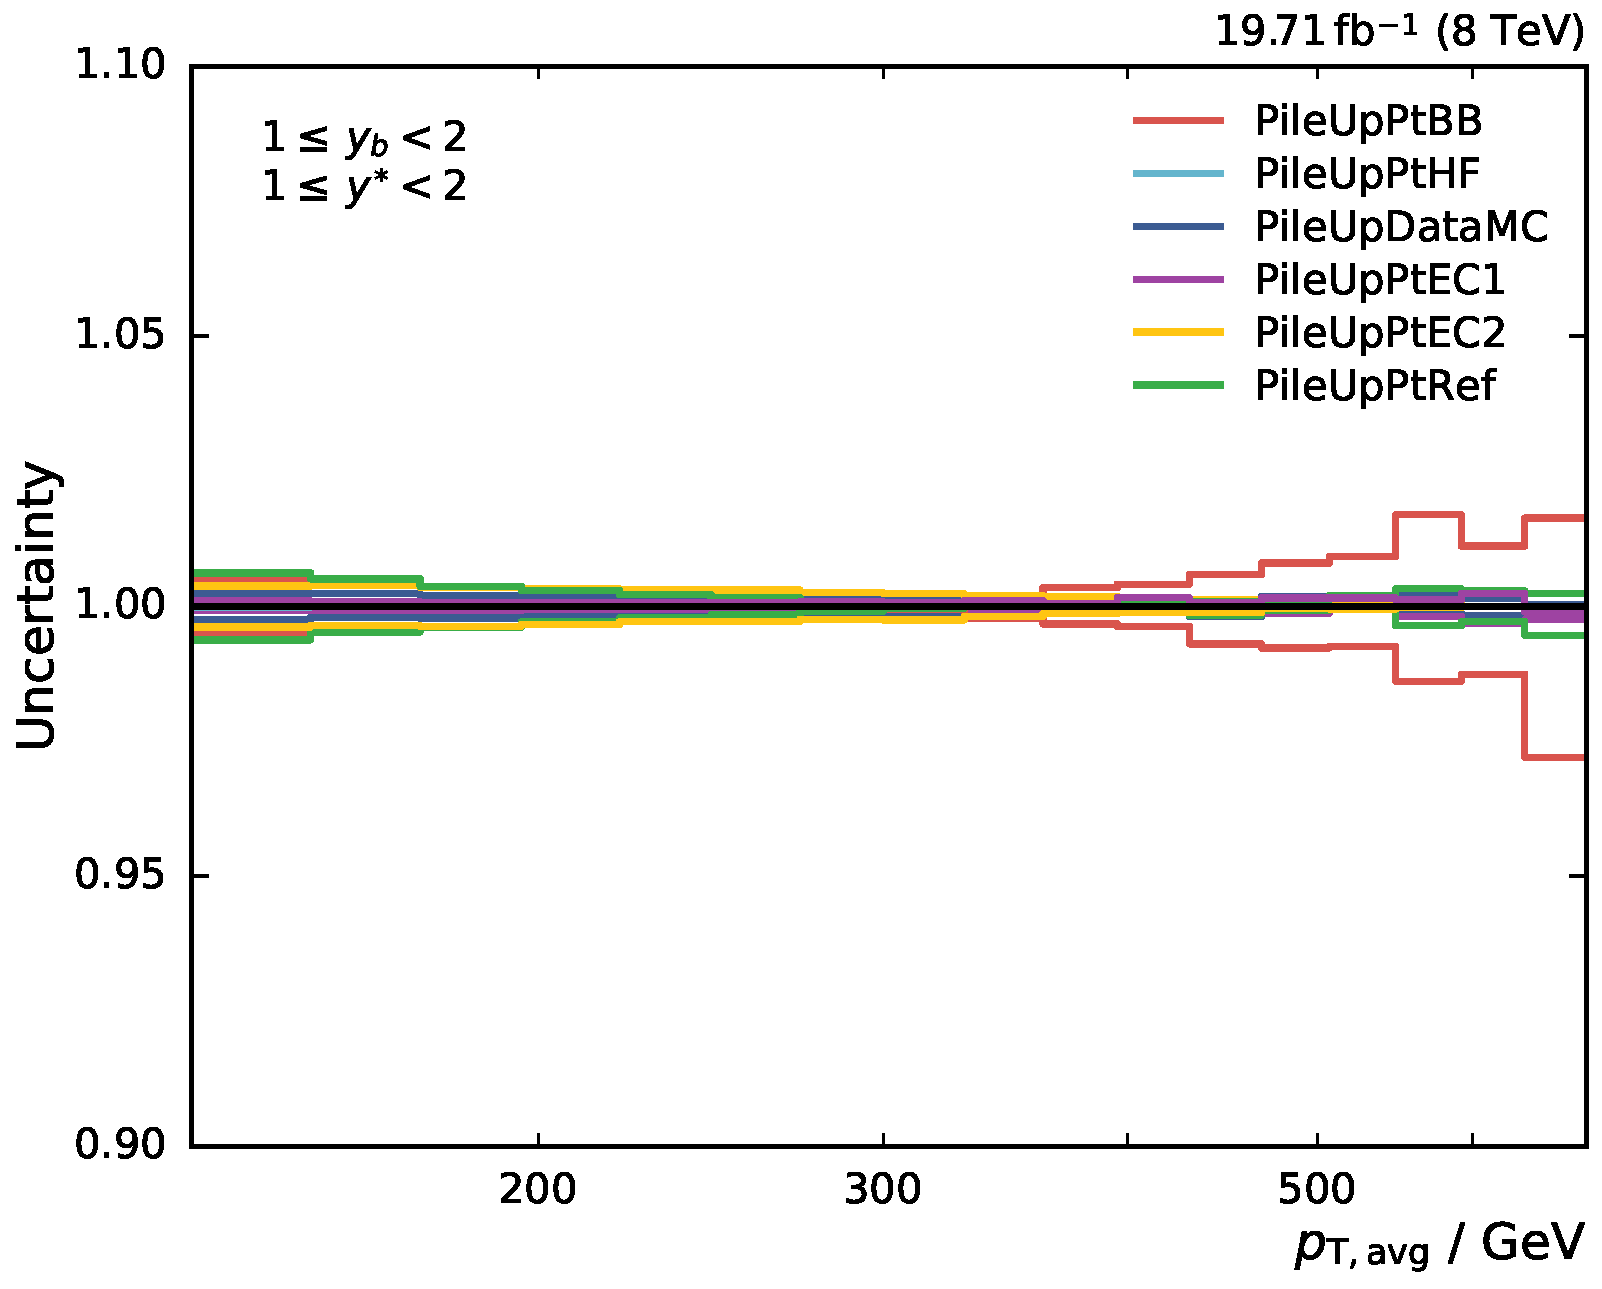
\includegraphics[width=0.49\textwidth]{figures/measurement/jec_relunc_5_yb1ys1.pdf}\hfill
    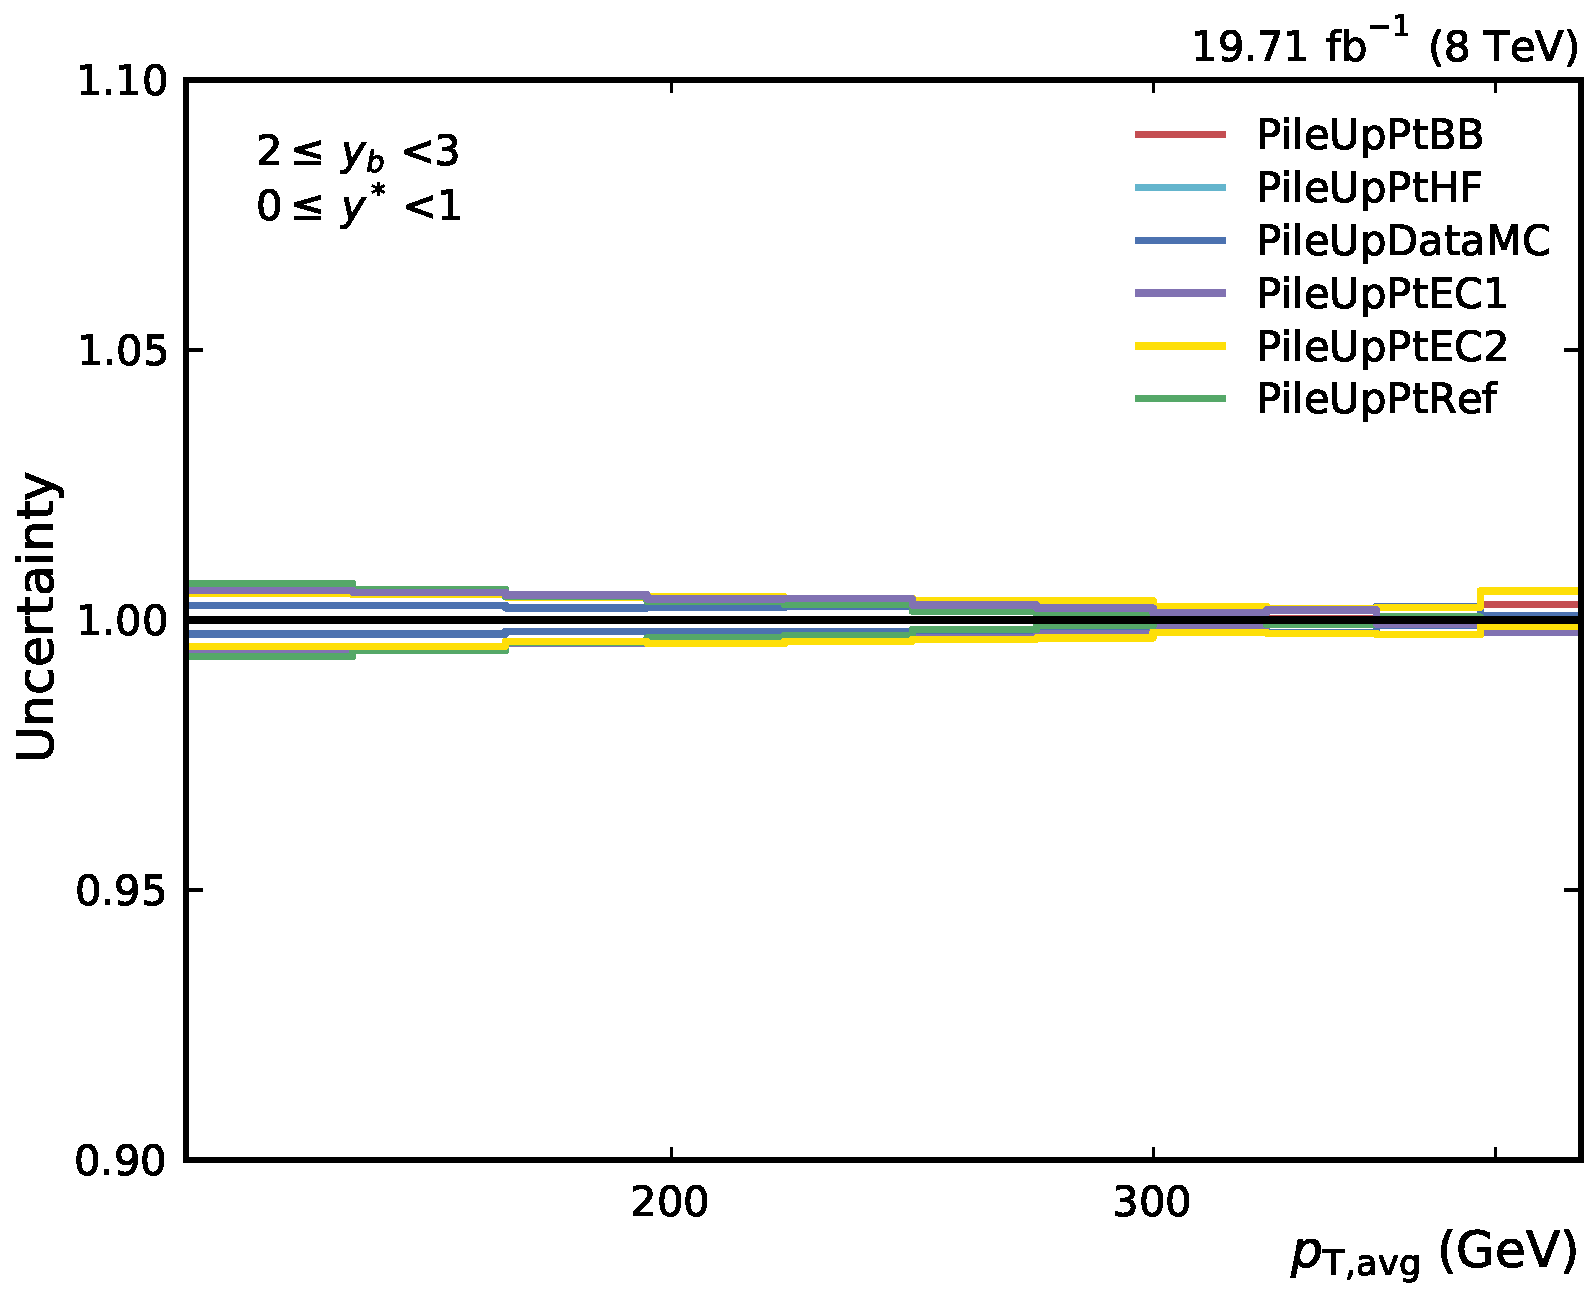
\includegraphics[width=0.49\textwidth]{figures/measurement/jec_relunc_5_yb2ys0.pdf}
    \caption[Split-up of JEC uncertainty sources: Part VI]{The relative size of the jet energy scale
             uncertainties for the sources PileUpPtBB, PileUpPtHF, PileUpDataMC,
             PileUpPtEC1, PileUpPtEC2, and PileUpPtRef are shown for all \ystar and \yboost bins.}
    \label{fig:jec_relunc_5}
\end{figure}


\section{Additional Data and Theory Comparisons}

\begin{figure}[htbp]
    \centering
    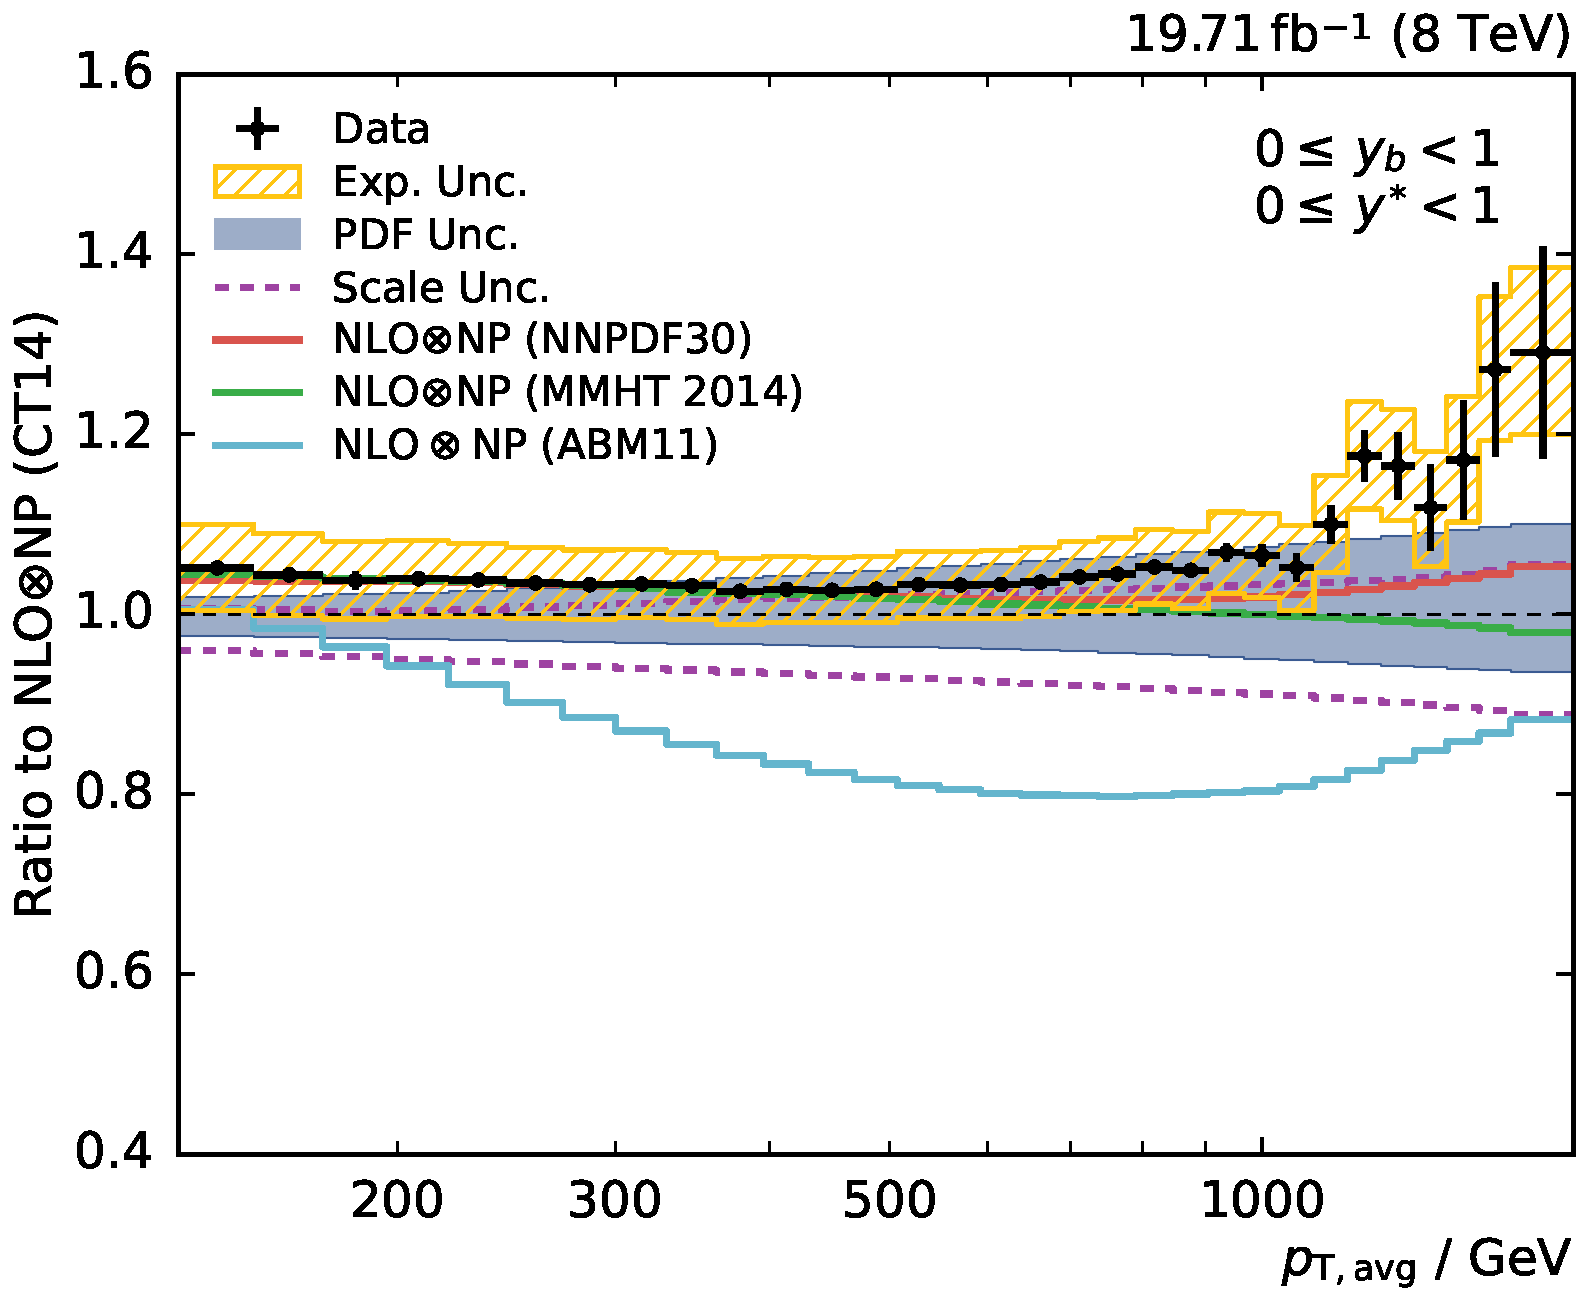
\includegraphics[width=0.45\textwidth]{figures/measurement/ratio_to_CT14nlo+np_totcomp_yb0ys0.pdf}\hfill
    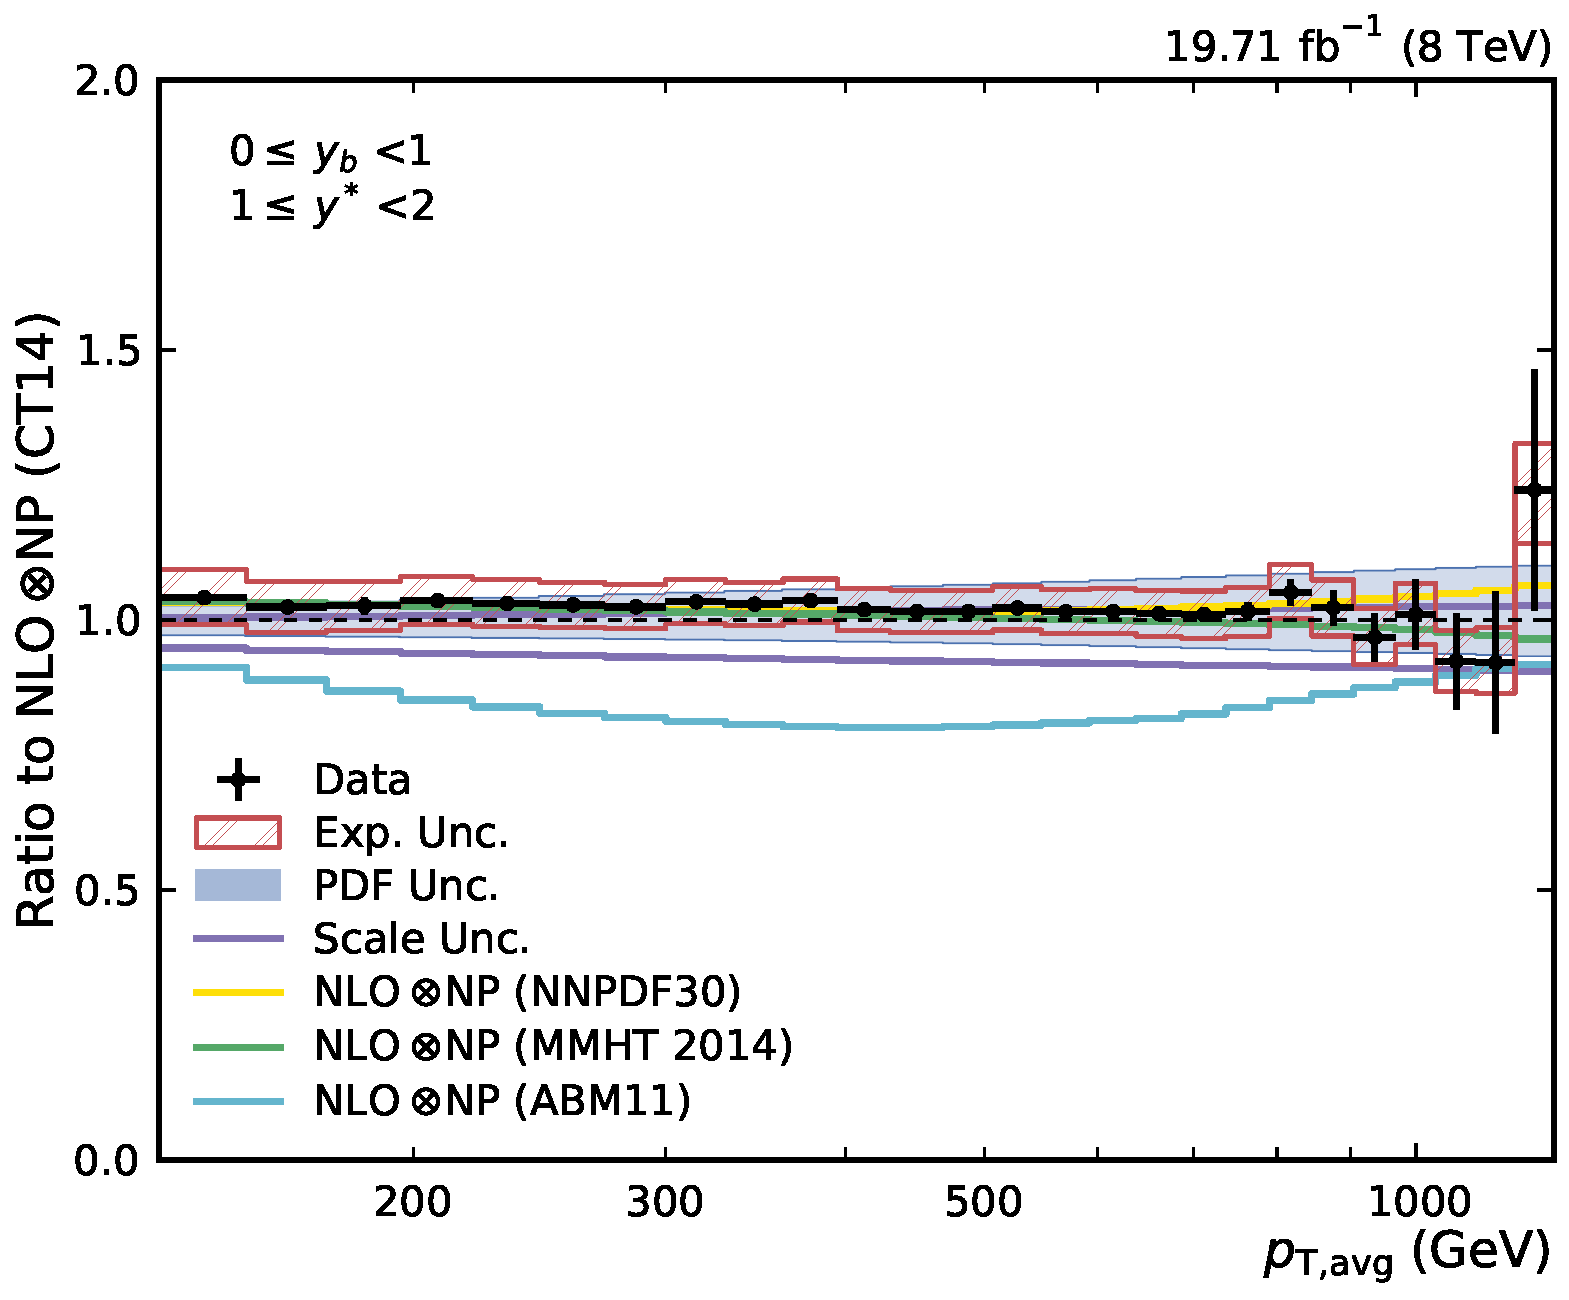
\includegraphics[width=0.45\textwidth]{figures/measurement/ratio_to_CT14nlo+np_totcomp_yb0ys1.pdf}
    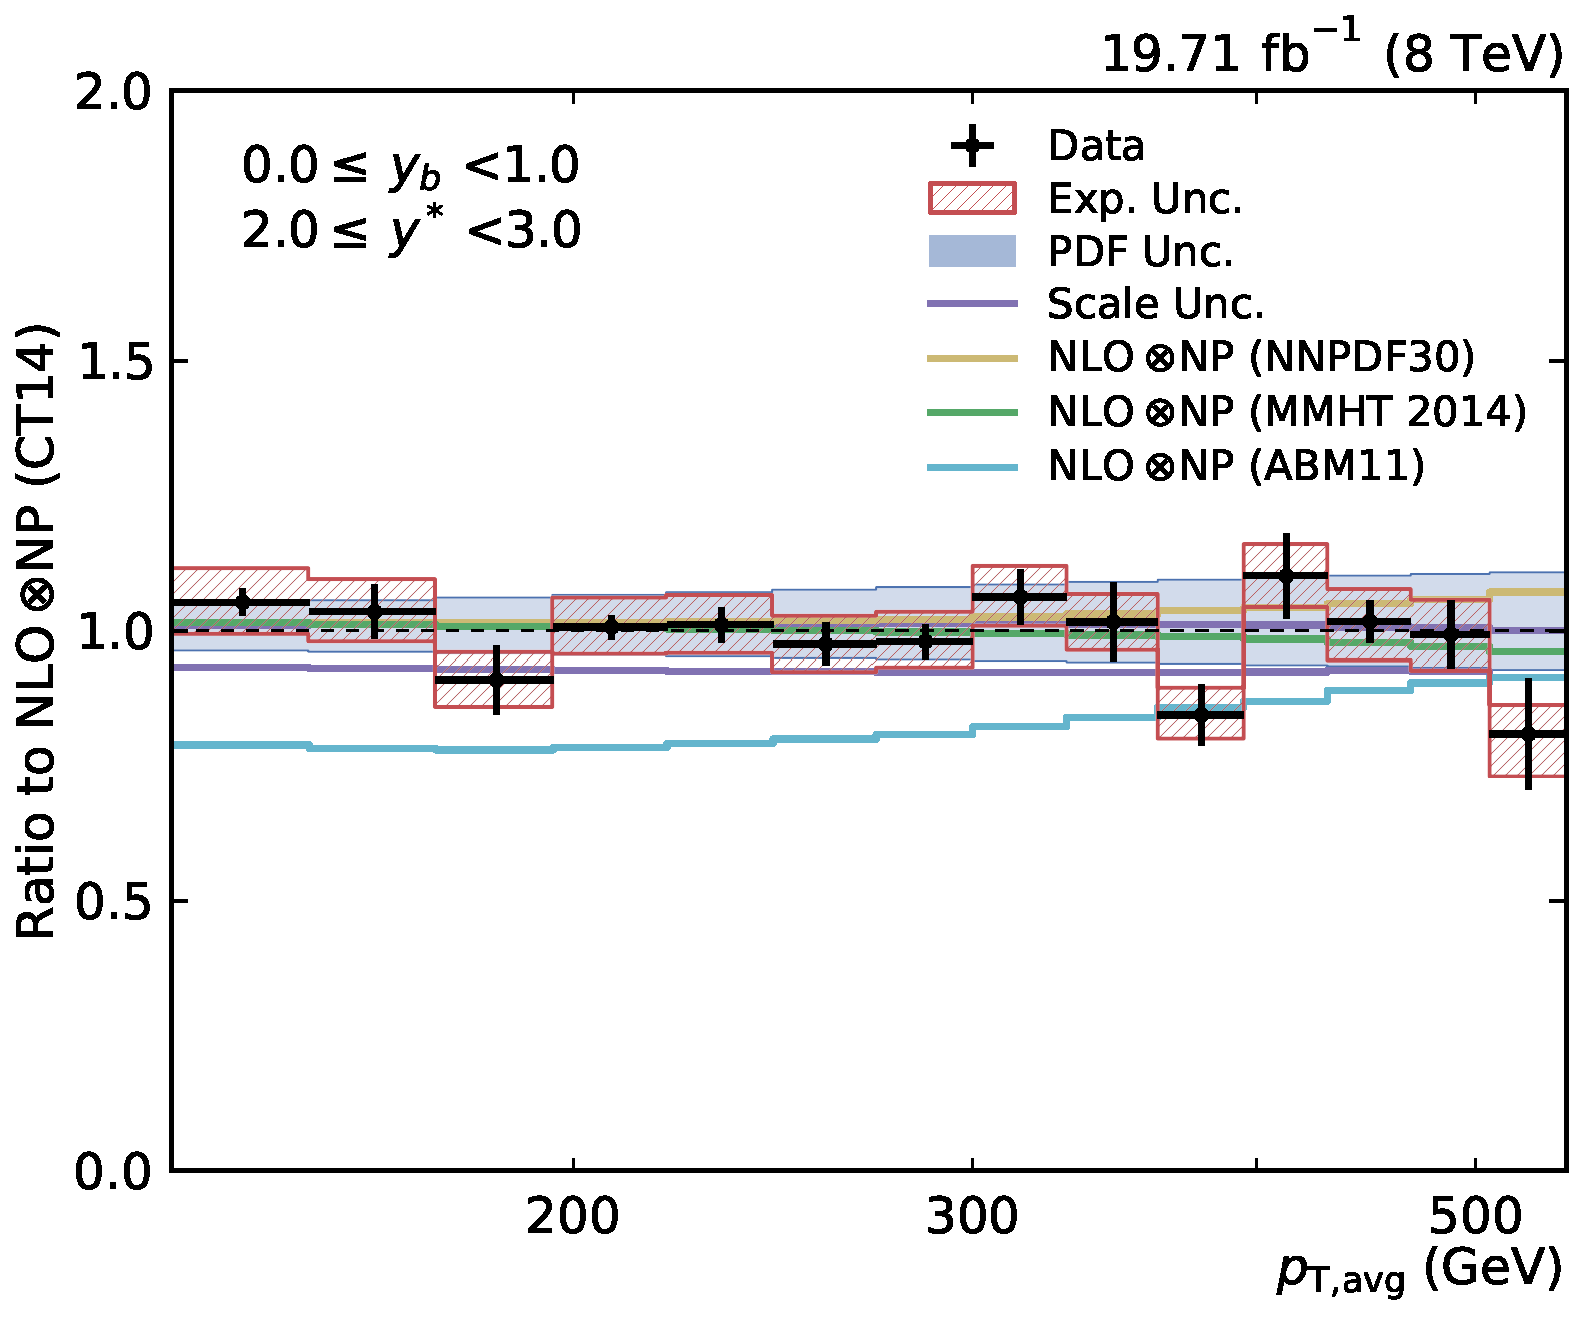
\includegraphics[width=0.45\textwidth]{figures/measurement/ratio_to_CT14nlo+np_totcomp_yb0ys2.pdf}\hfill
    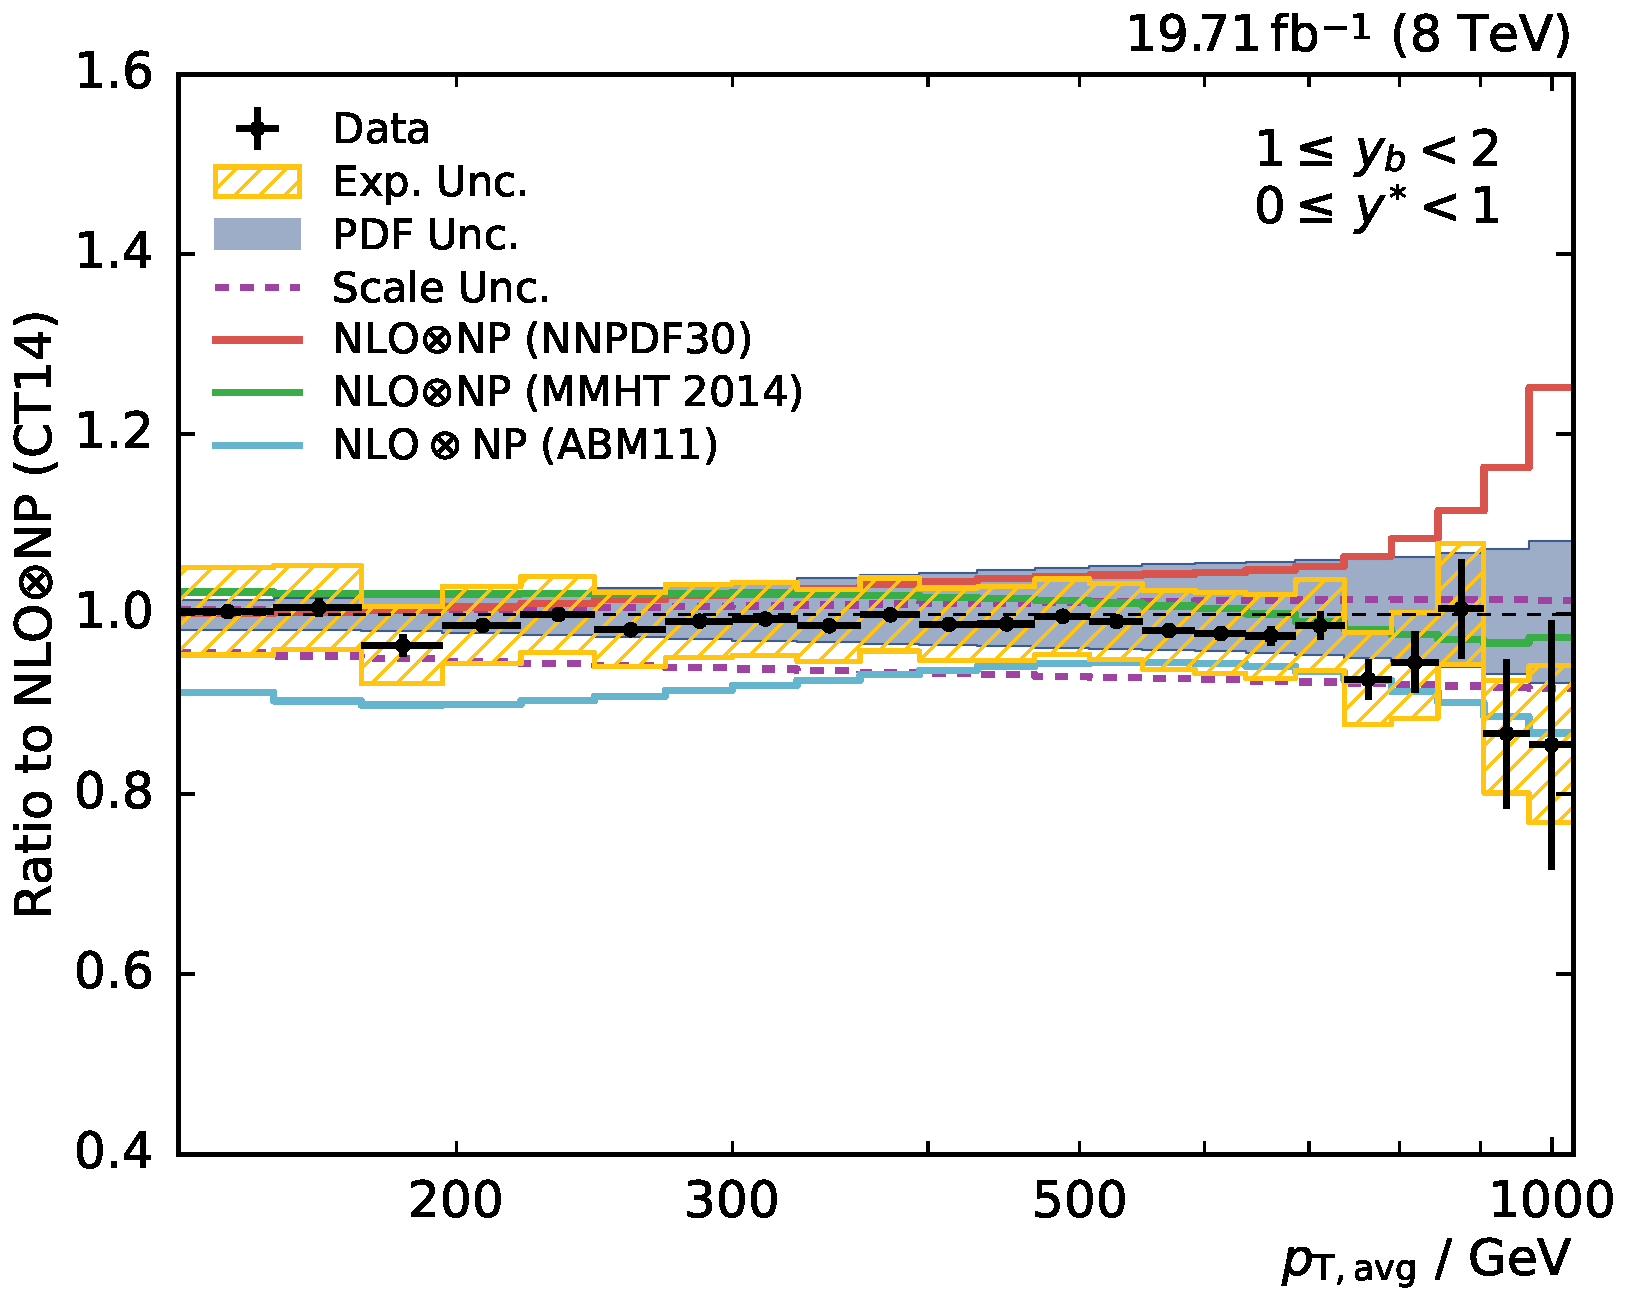
\includegraphics[width=0.45\textwidth]{figures/measurement/ratio_to_CT14nlo+np_totcomp_yb1ys0.pdf}
    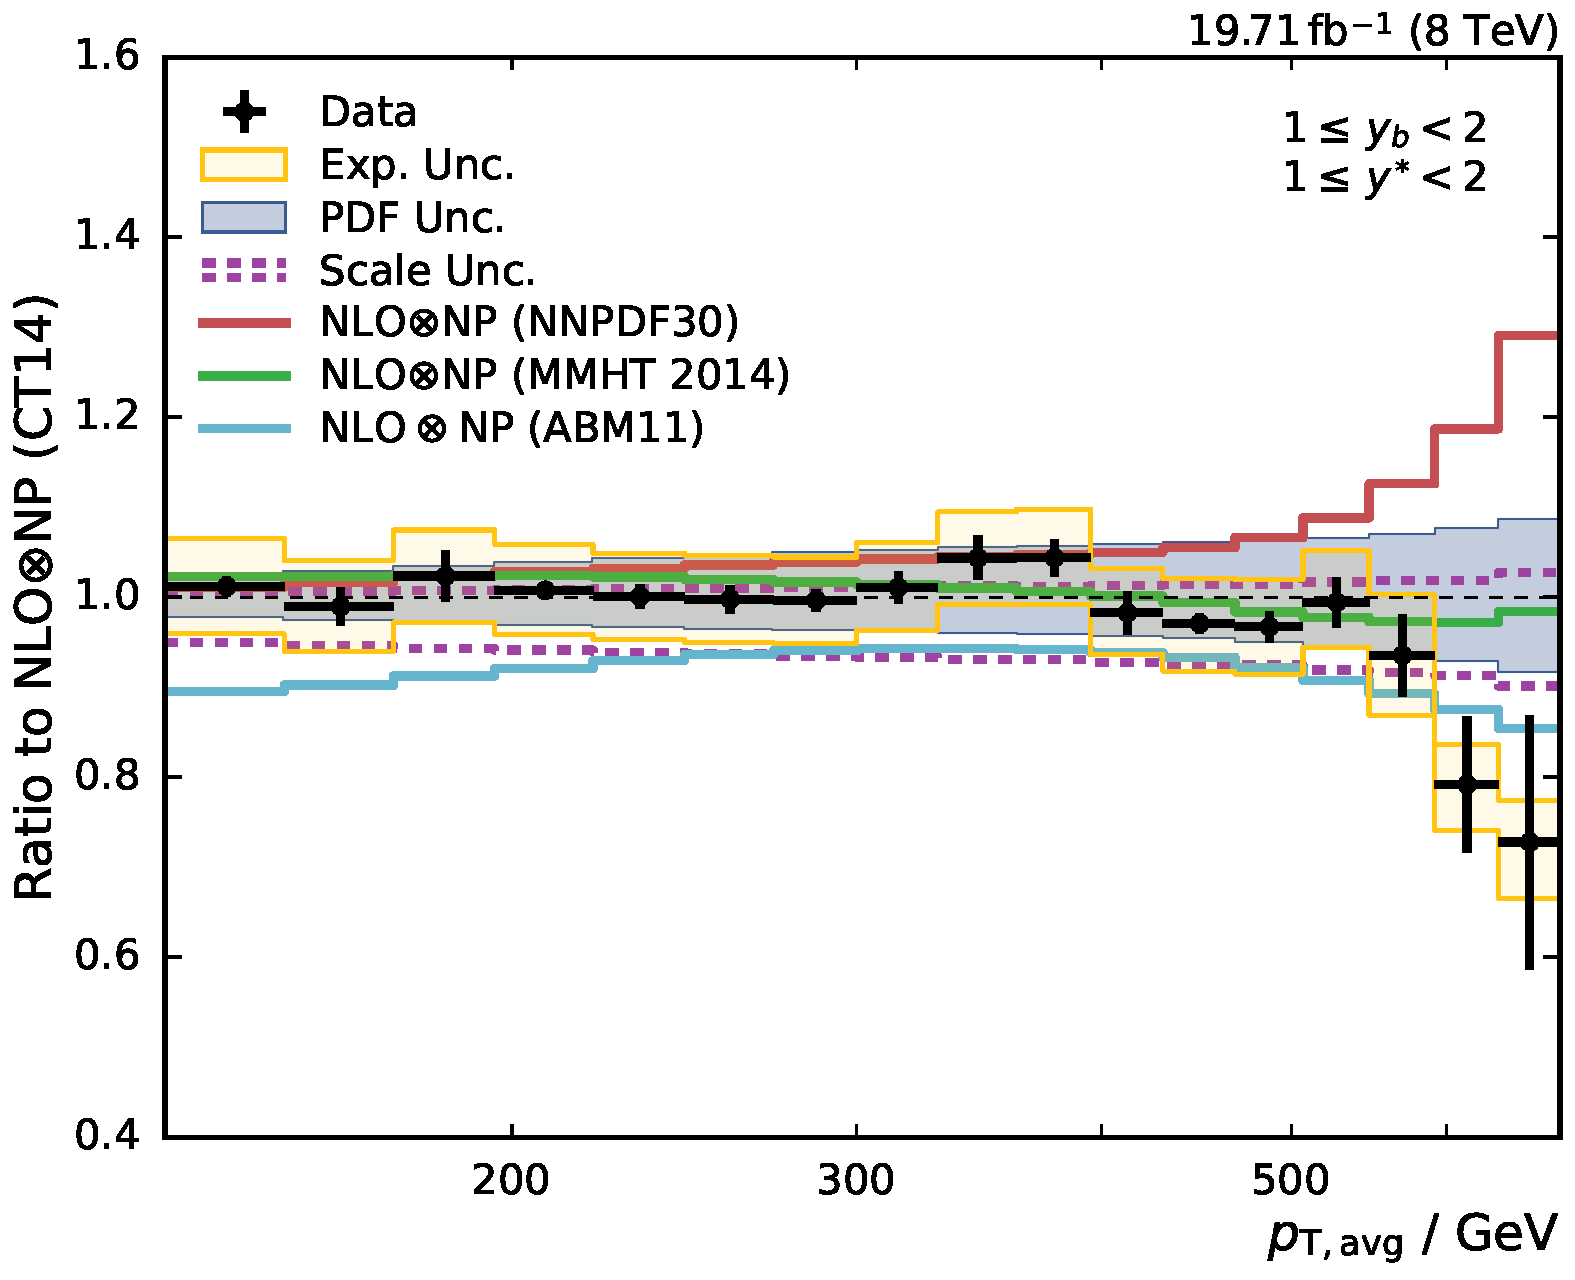
\includegraphics[width=0.45\textwidth]{figures/measurement/ratio_to_CT14nlo+np_totcomp_yb1ys1.pdf}\hfill
    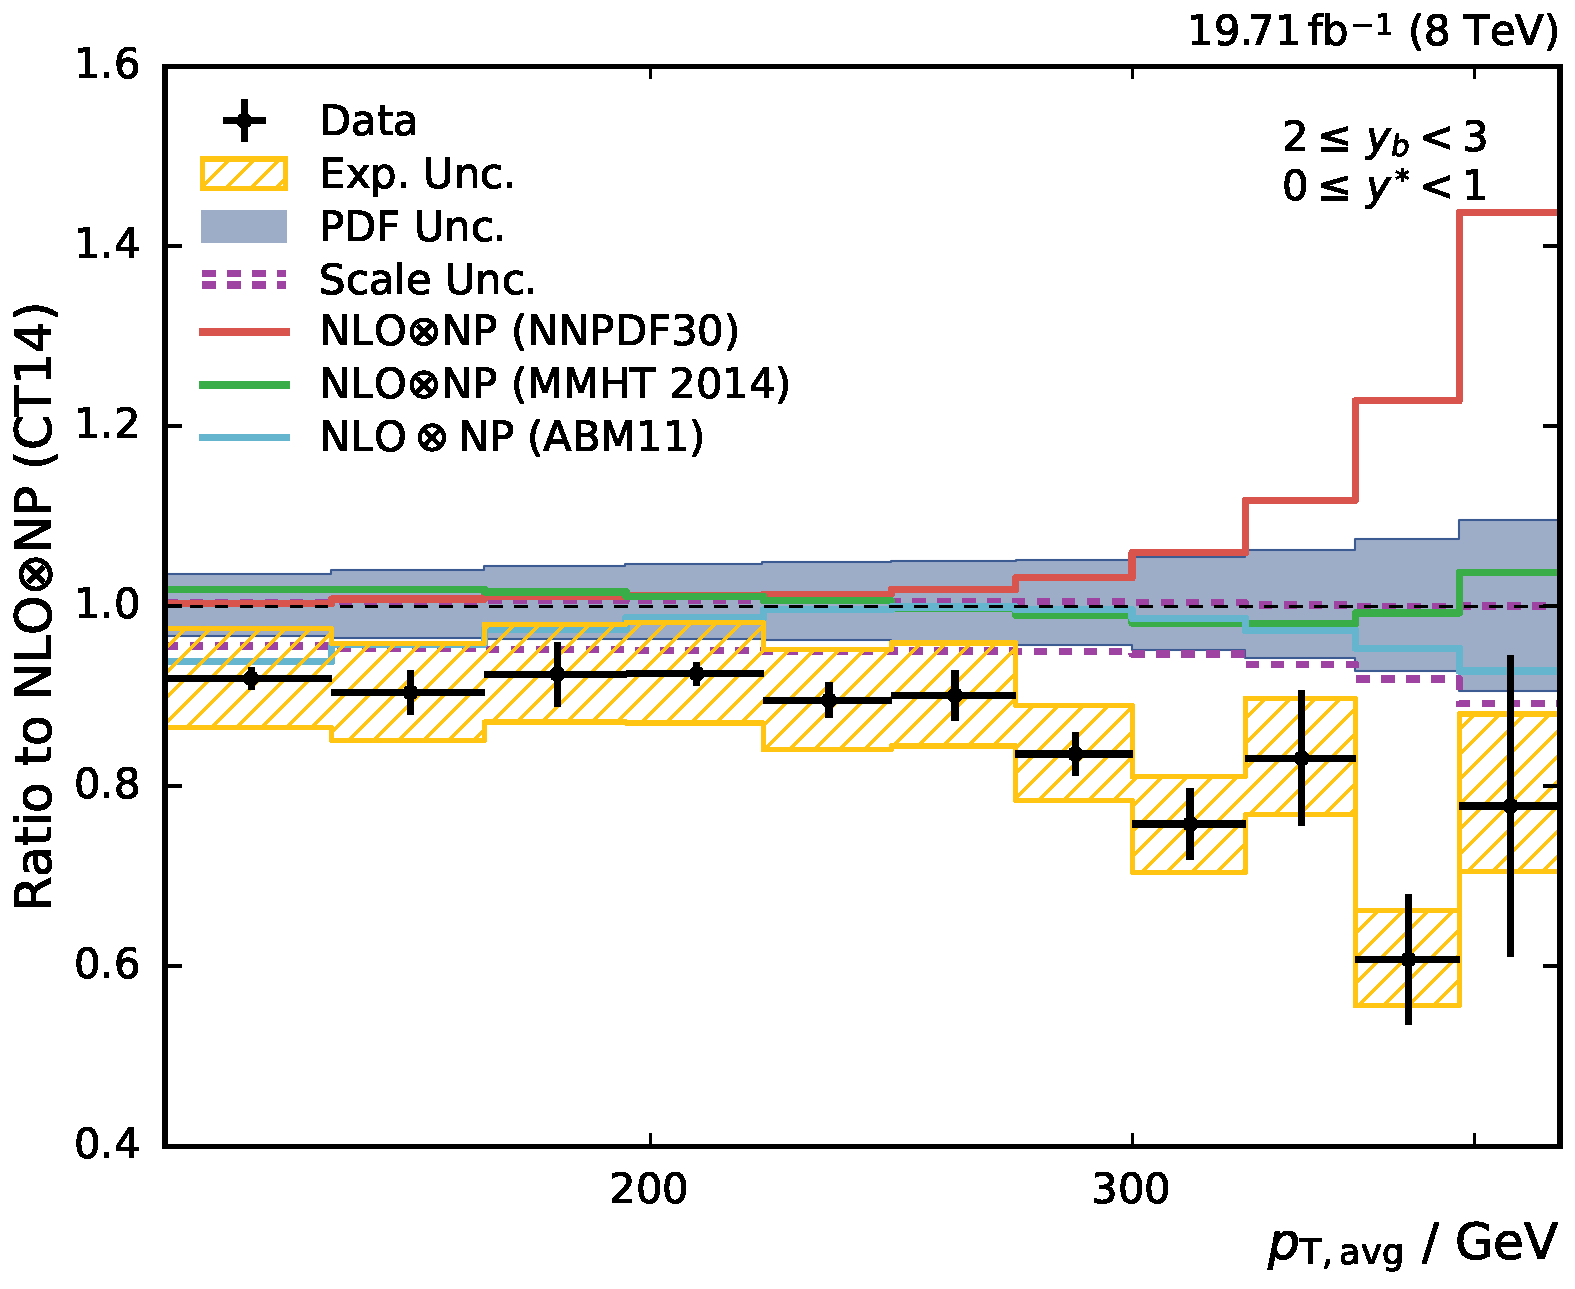
\includegraphics[width=0.45\textwidth]{figures/measurement/ratio_to_CT14nlo+np_totcomp_yb2ys0.pdf}
    \caption[Ratio of the cross section to CT14 NLO]{
    Ratio of the triple-differential dijet cross sections to the theoretical
    prediction using the central value of the CT14 NLO PDF set for each bin in \ystar
    and \yboost respectively. The data points including statistical uncertainty are
    indicated by markers, the total experimental uncertainty is represented by the
    hatched band. The solid blue band indicates the PDF uncertainty and the
    continous colored lines the predictions of the cross sections calculated with
    other PDF sets.}
    \label{fig:ratio_ct14_nlo}
\end{figure}


\begin{figure}[htbp]
    \centering
    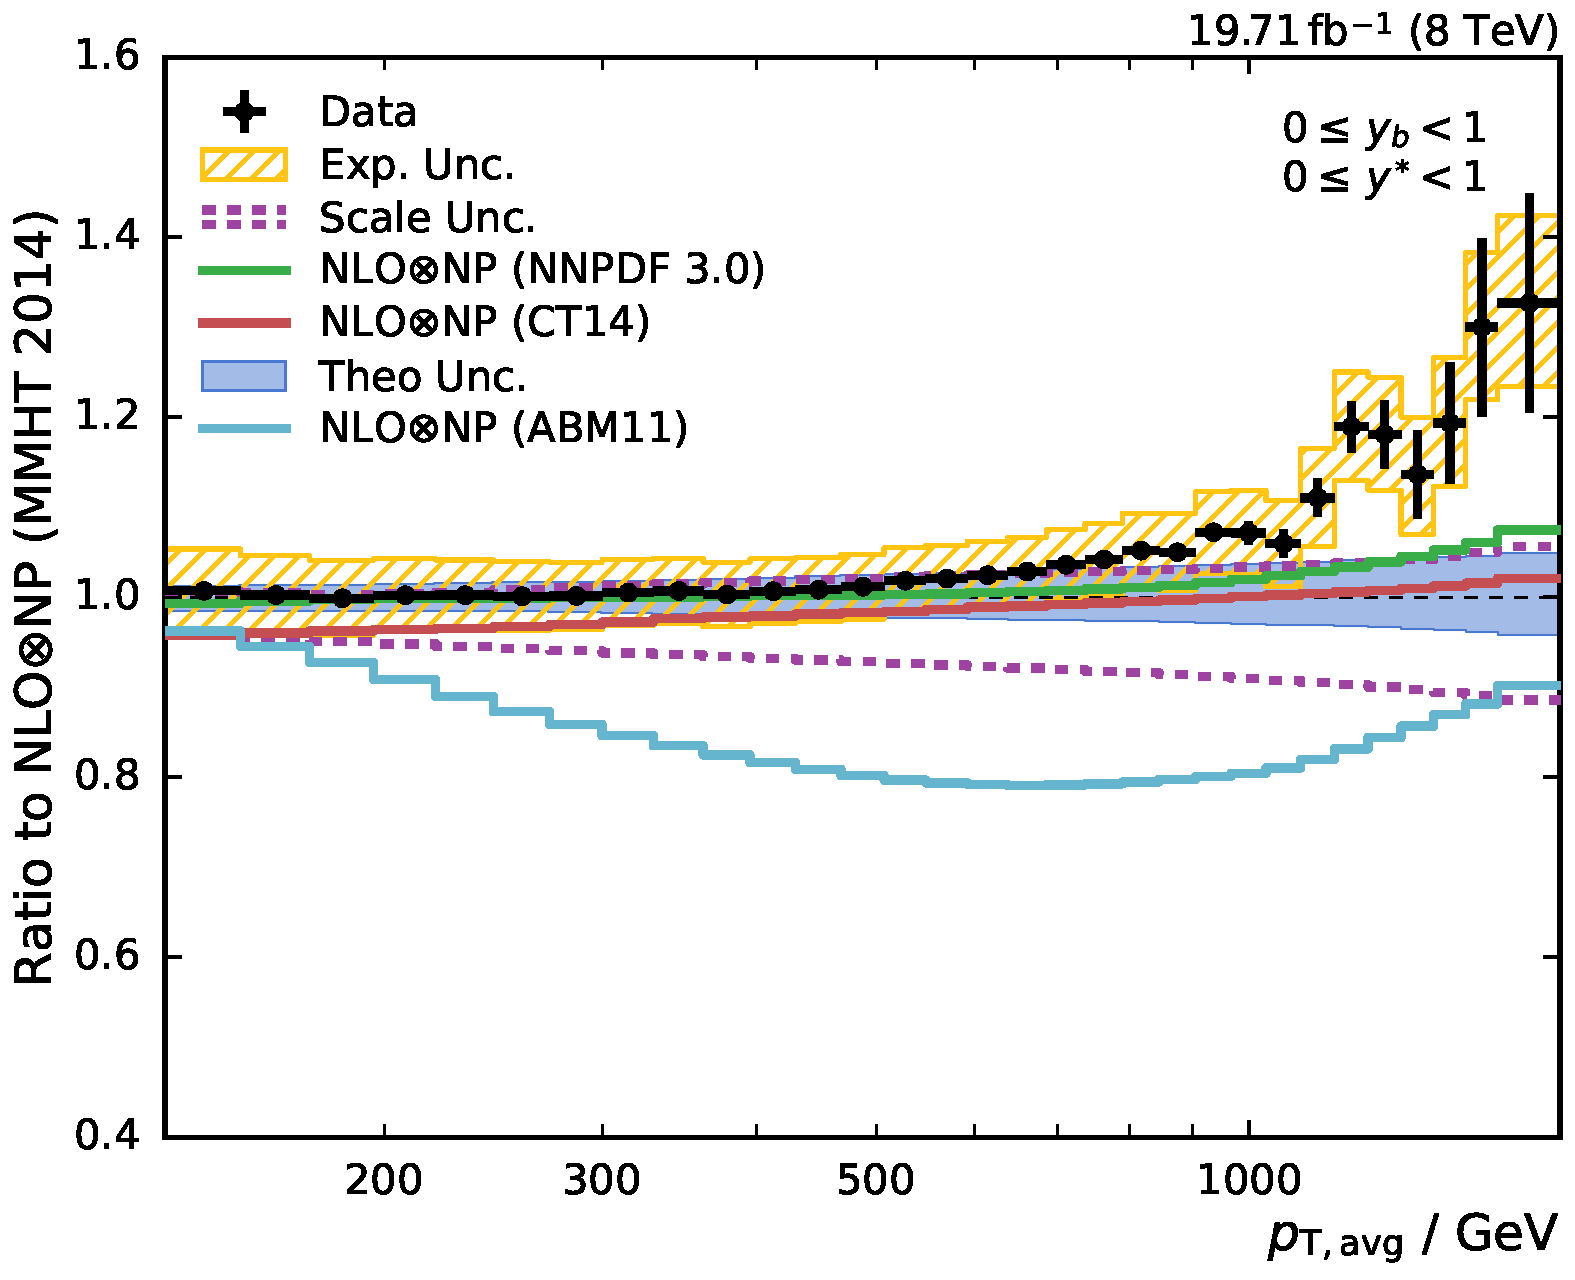
\includegraphics[width=0.45\textwidth]{figures/measurement/ratio_to_MMHT2014+np_totcomp_yb0ys0.pdf}\hfill
    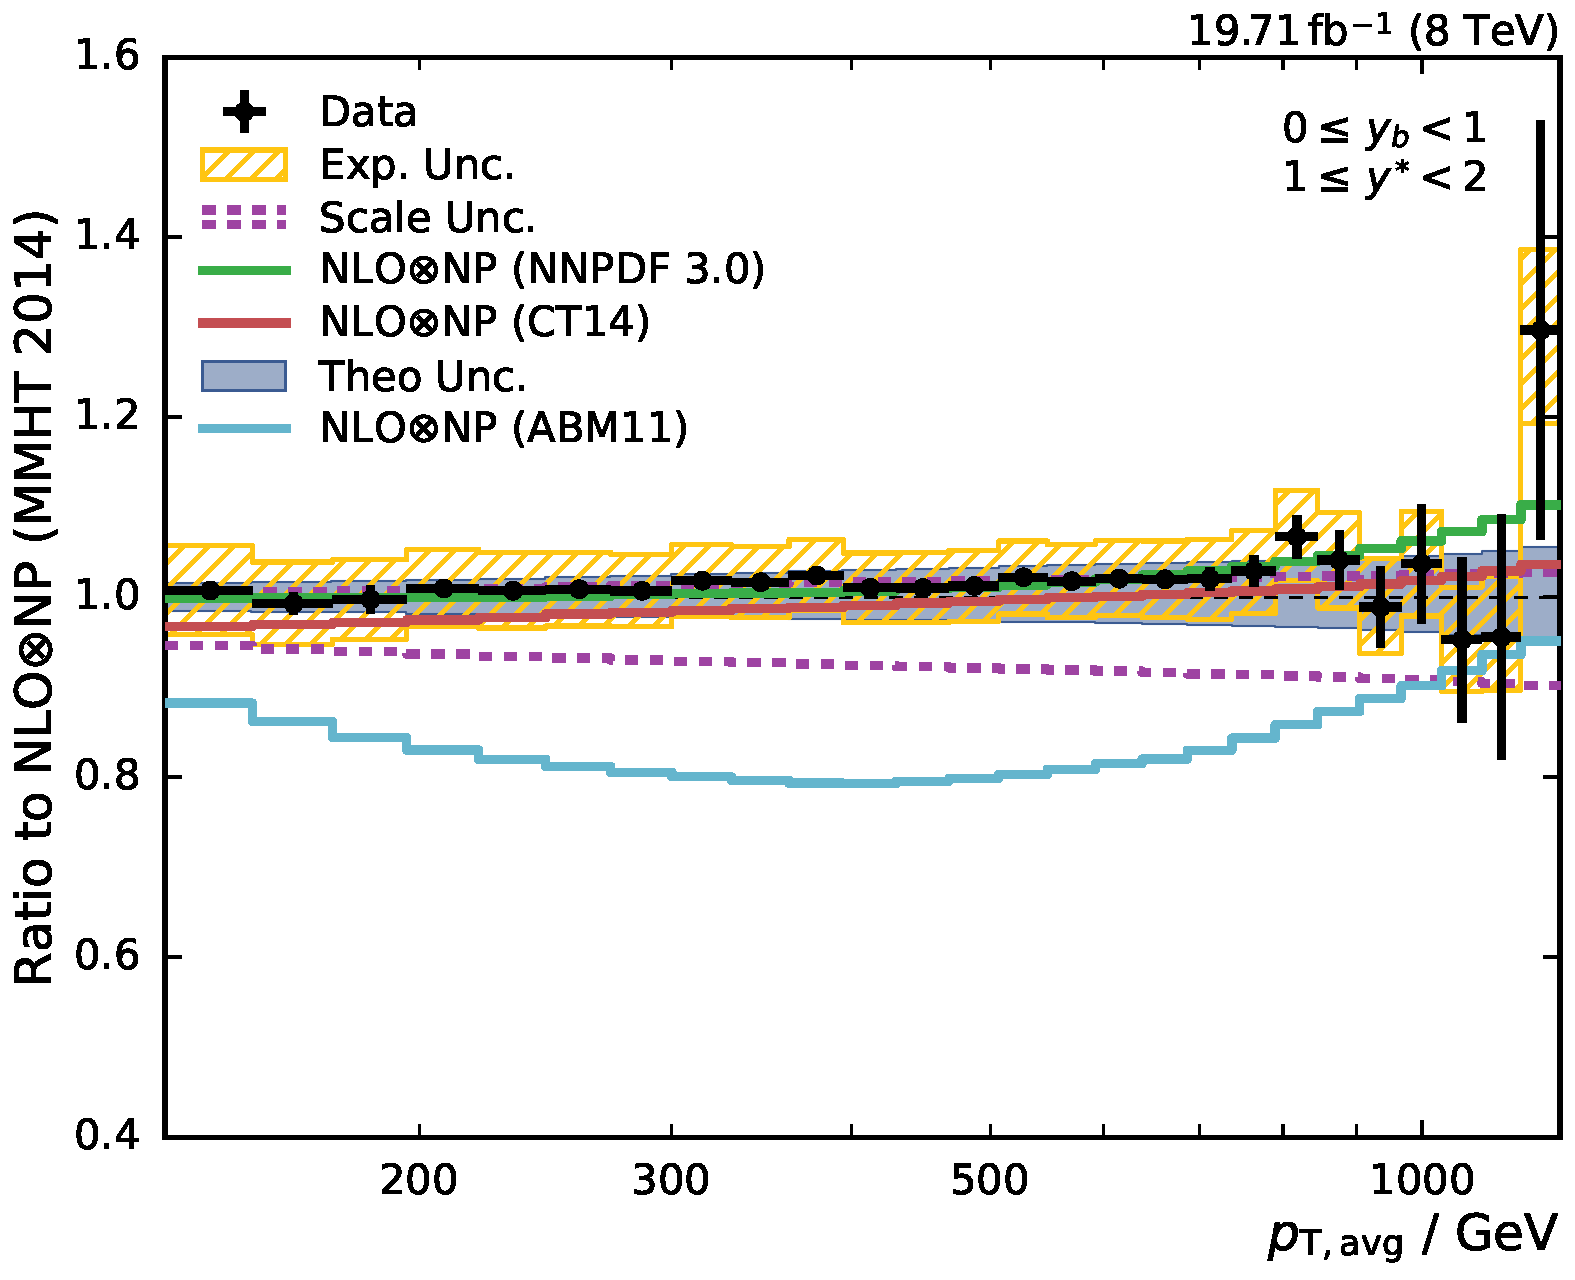
\includegraphics[width=0.45\textwidth]{figures/measurement/ratio_to_MMHT2014+np_totcomp_yb0ys1.pdf}
    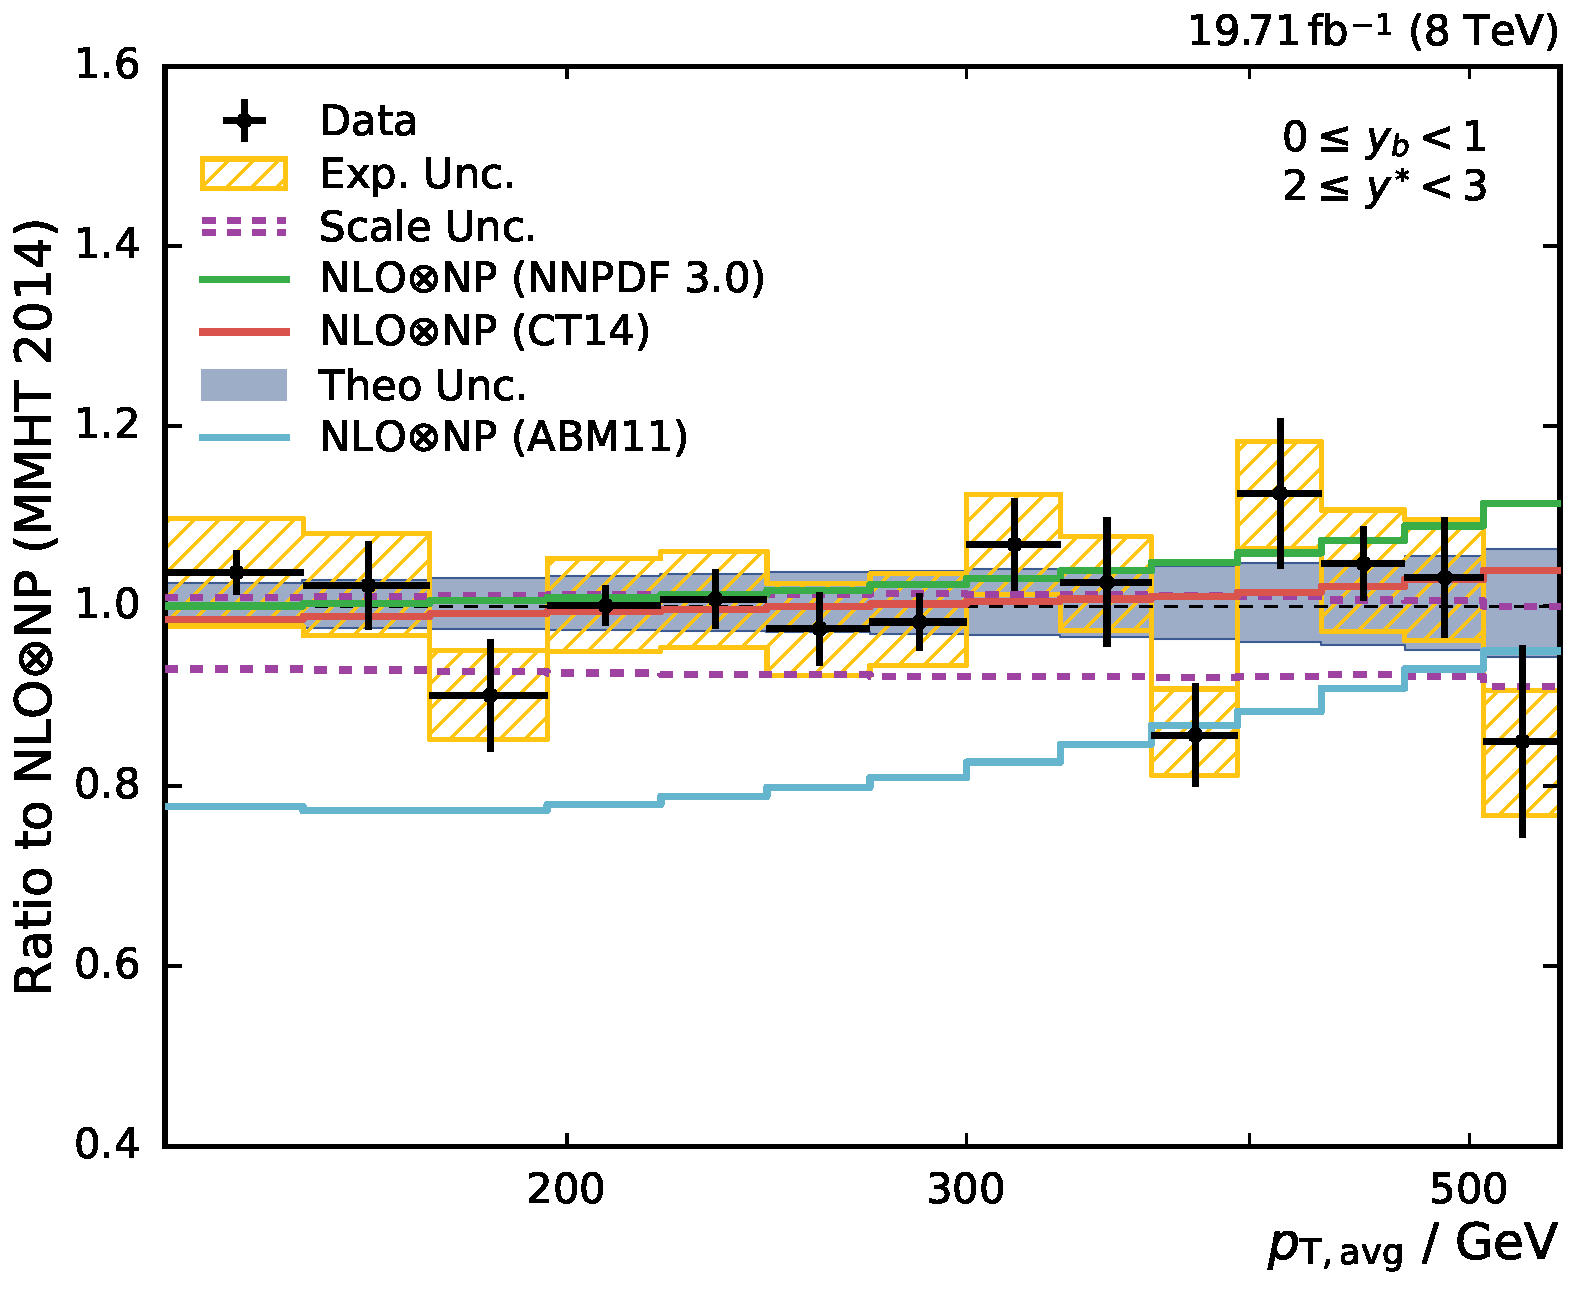
\includegraphics[width=0.45\textwidth]{figures/measurement/ratio_to_MMHT2014+np_totcomp_yb0ys2.pdf}\hfill
    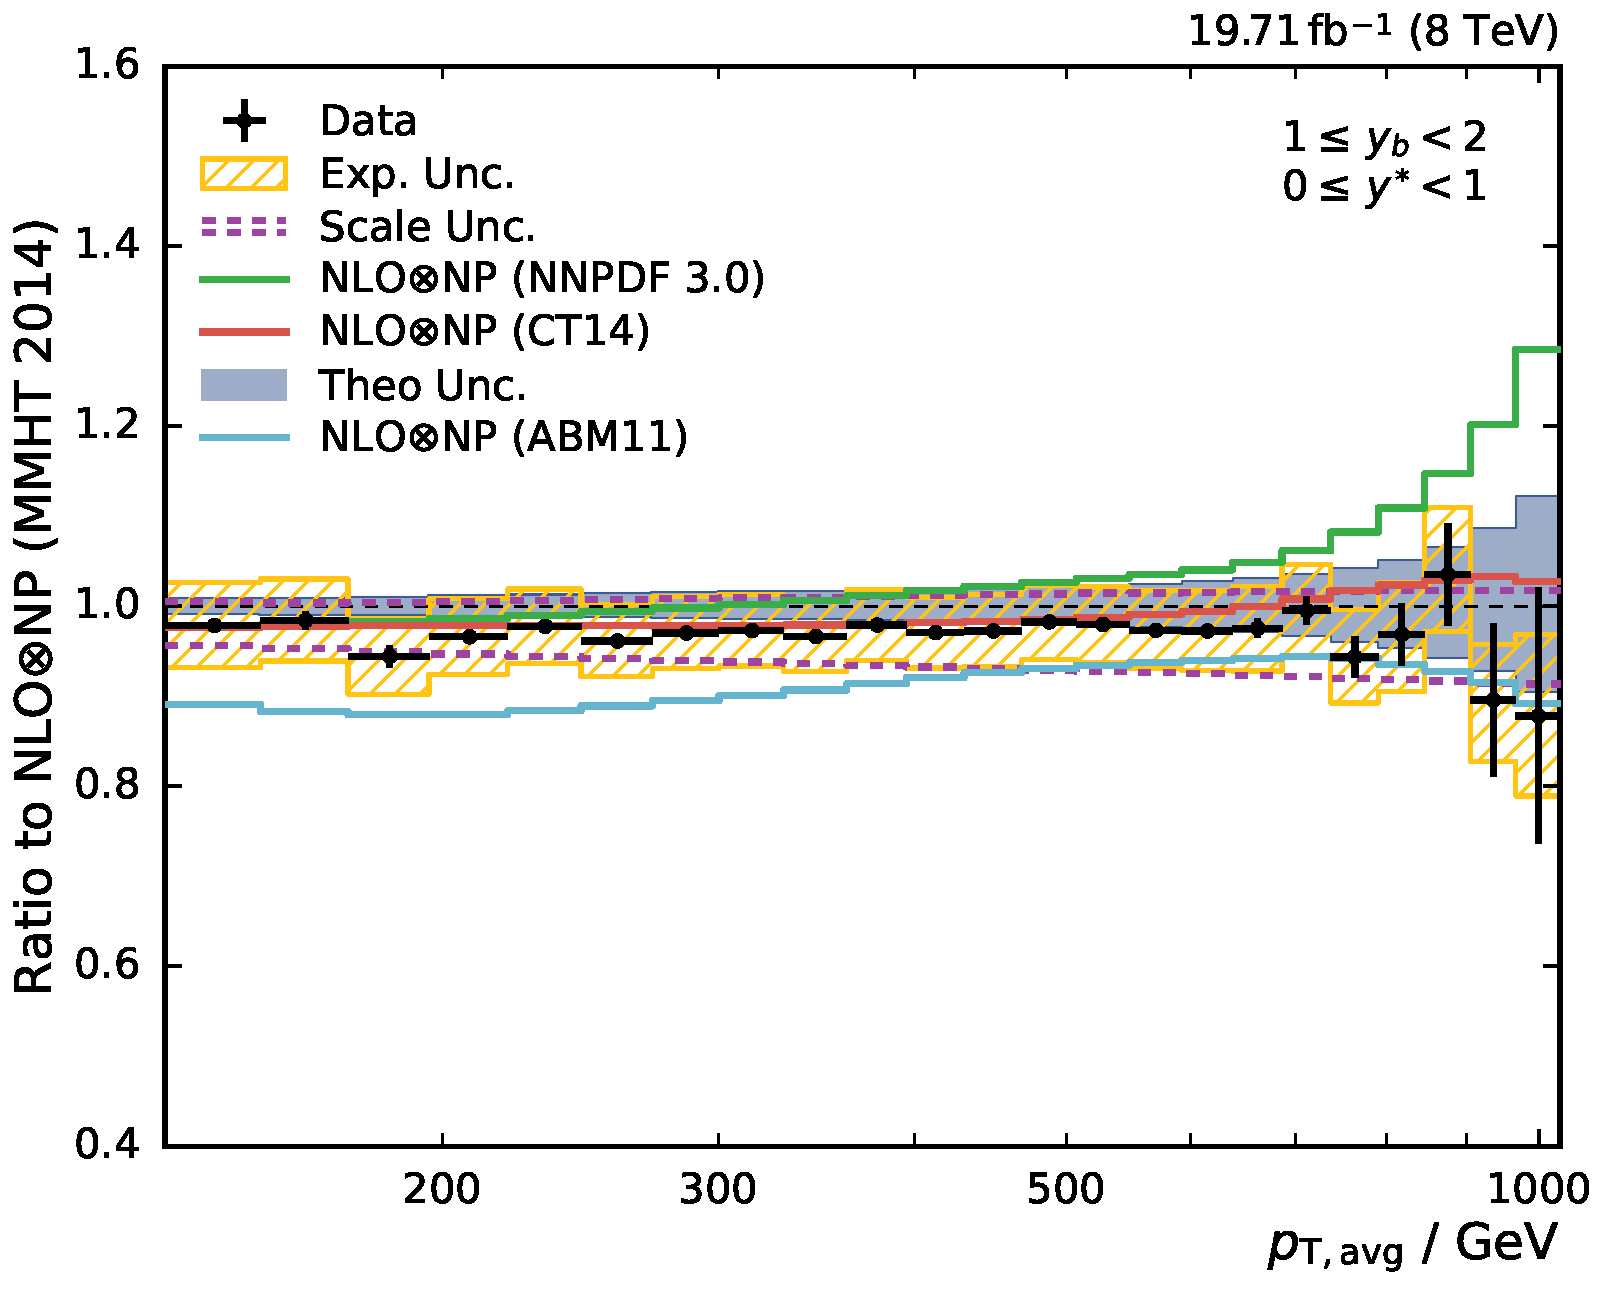
\includegraphics[width=0.45\textwidth]{figures/measurement/ratio_to_MMHT2014+np_totcomp_yb1ys0.pdf}
    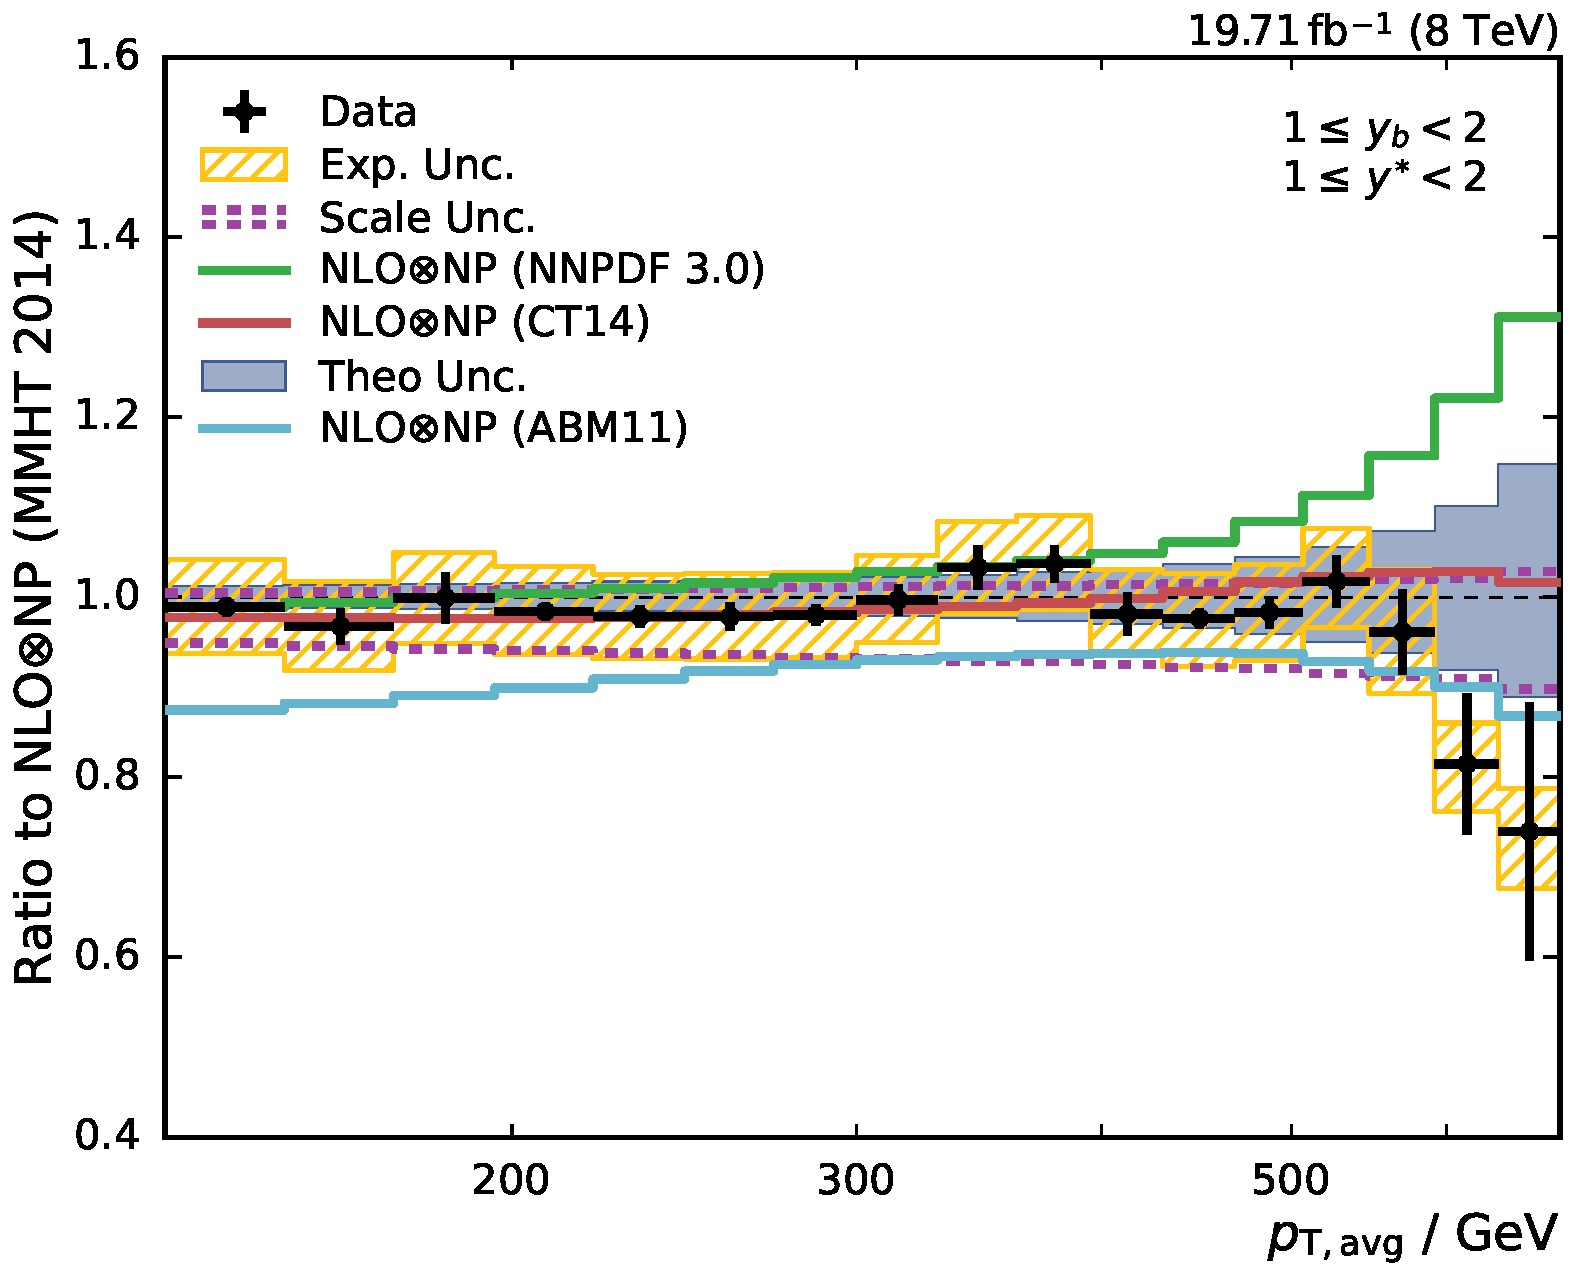
\includegraphics[width=0.45\textwidth]{figures/measurement/ratio_to_MMHT2014+np_totcomp_yb1ys1.pdf}\hfill
    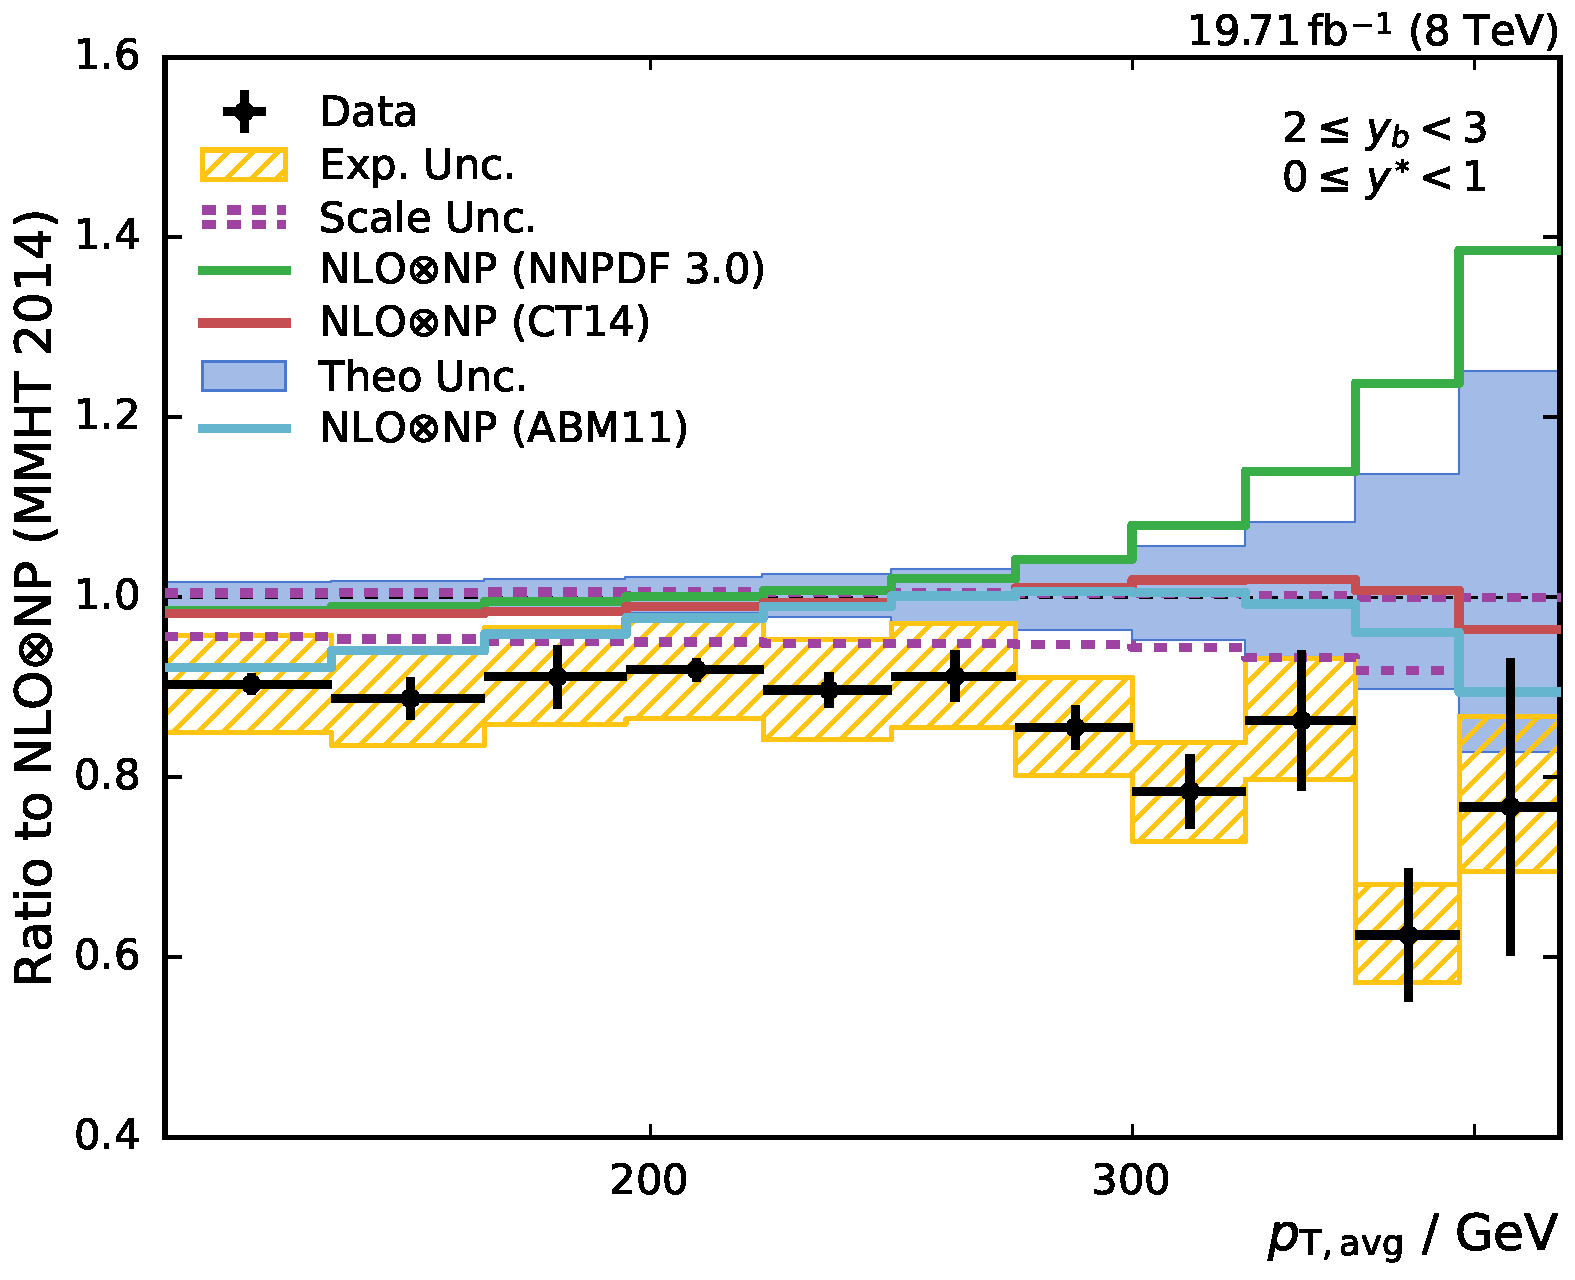
\includegraphics[width=0.45\textwidth]{figures/measurement/ratio_to_MMHT2014+np_totcomp_yb2ys0.pdf}
    \caption[Ratio of the cross section to MMHT2014 NLO]{
    Ratio of the triple-differential dijet cross sections to the theoretical
    prediction using the central value of the MMHT 2014 NLO PDF set for each bin in \ystar
    and \yboost respectively. The data points including statistical uncertainty are
    indicated by markers, the total experimental uncertainty is represented by the
    hatched band. The solid blue band indicates the PDF uncertainty and the
    continous colored lines the predictions of the cross sections calculated with
    other PDF sets.}
    \label{fig:ratio_mmht_nlo}
\end{figure}


\section{PDF Correlations}

Additional material for the correlation studies of
Sec.~\ref{sec:pdf_sensitivity}.

\begin{figure}[htbp]
    \centering
    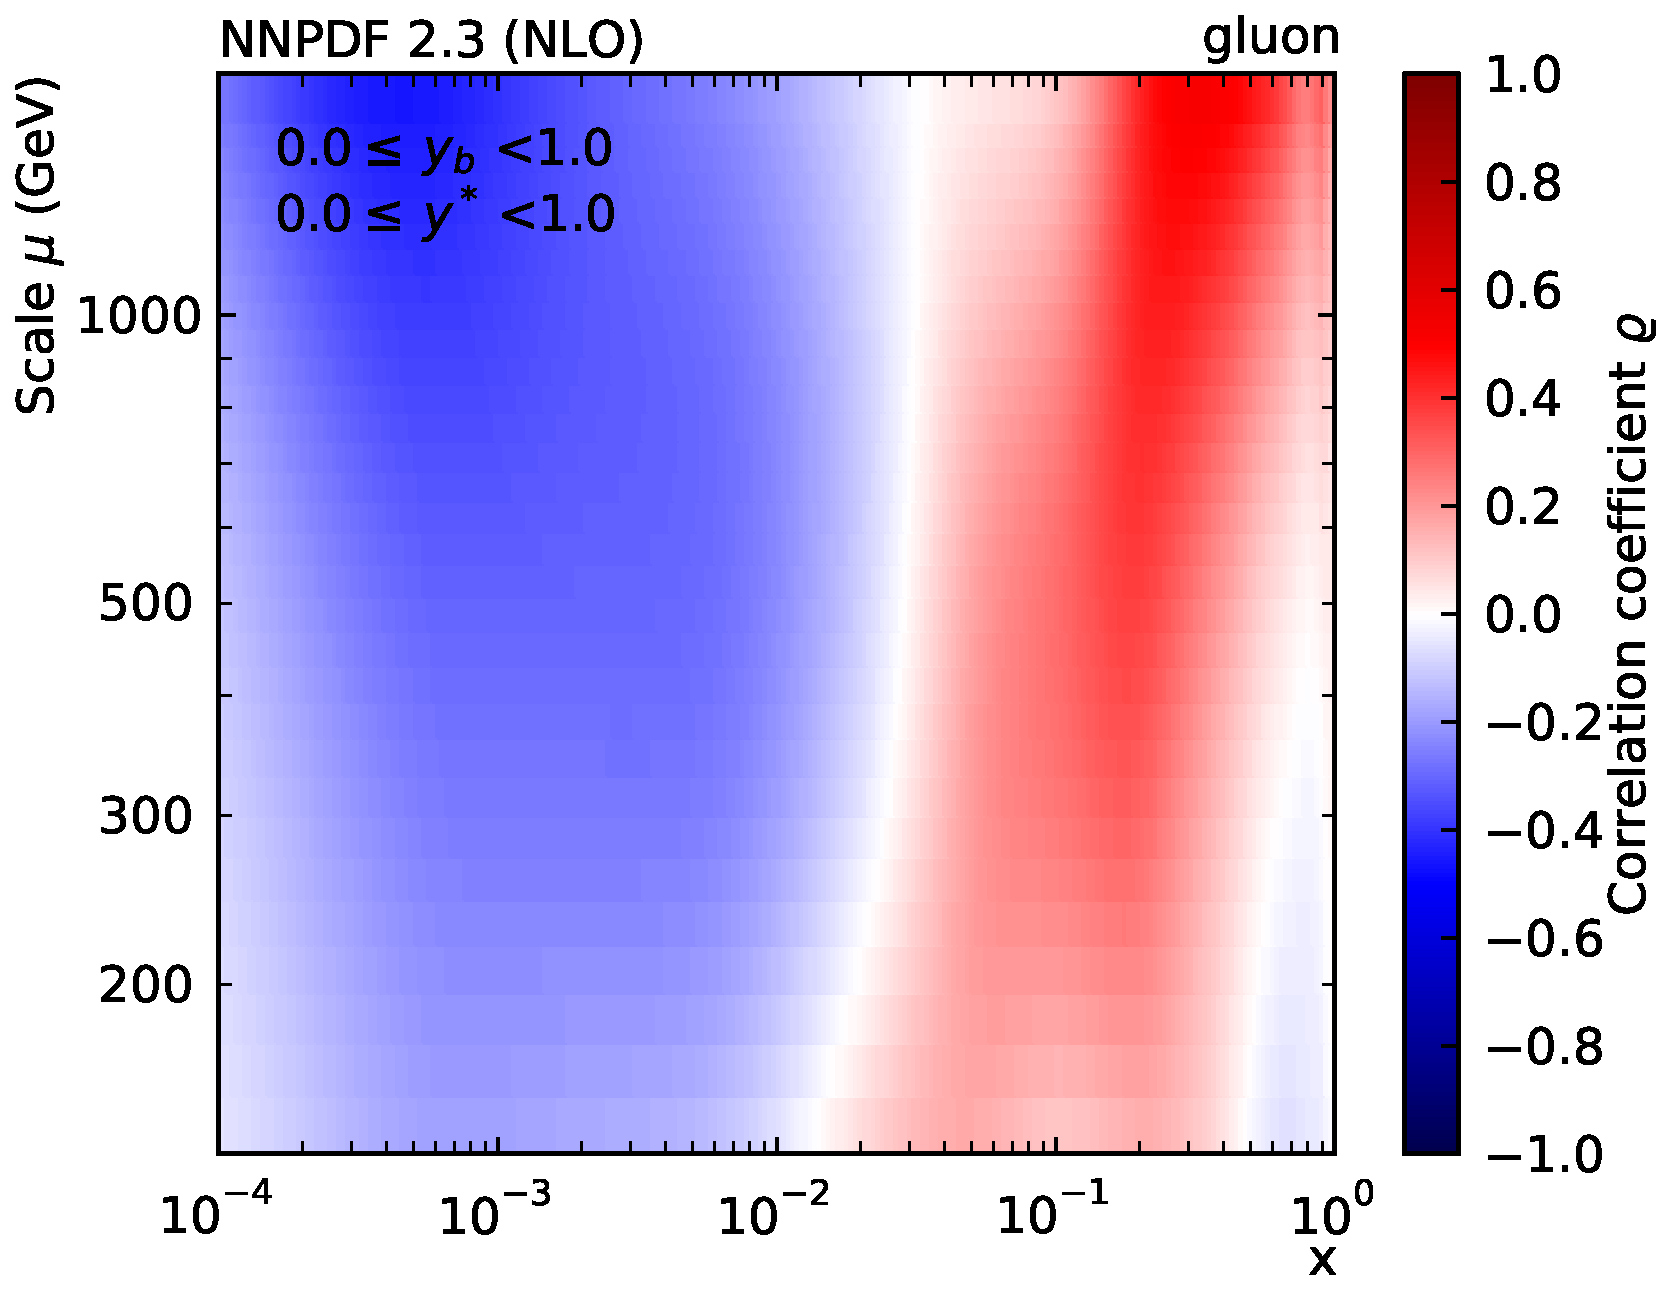
\includegraphics[width=0.49\textwidth]{figures/pdf_constraints/corr_PTMAXEXPYS_YBYS_NLO_FINALBINS_NNPDF23_gluon_ys0_0yb0_0_cl.pdf}\hfill
    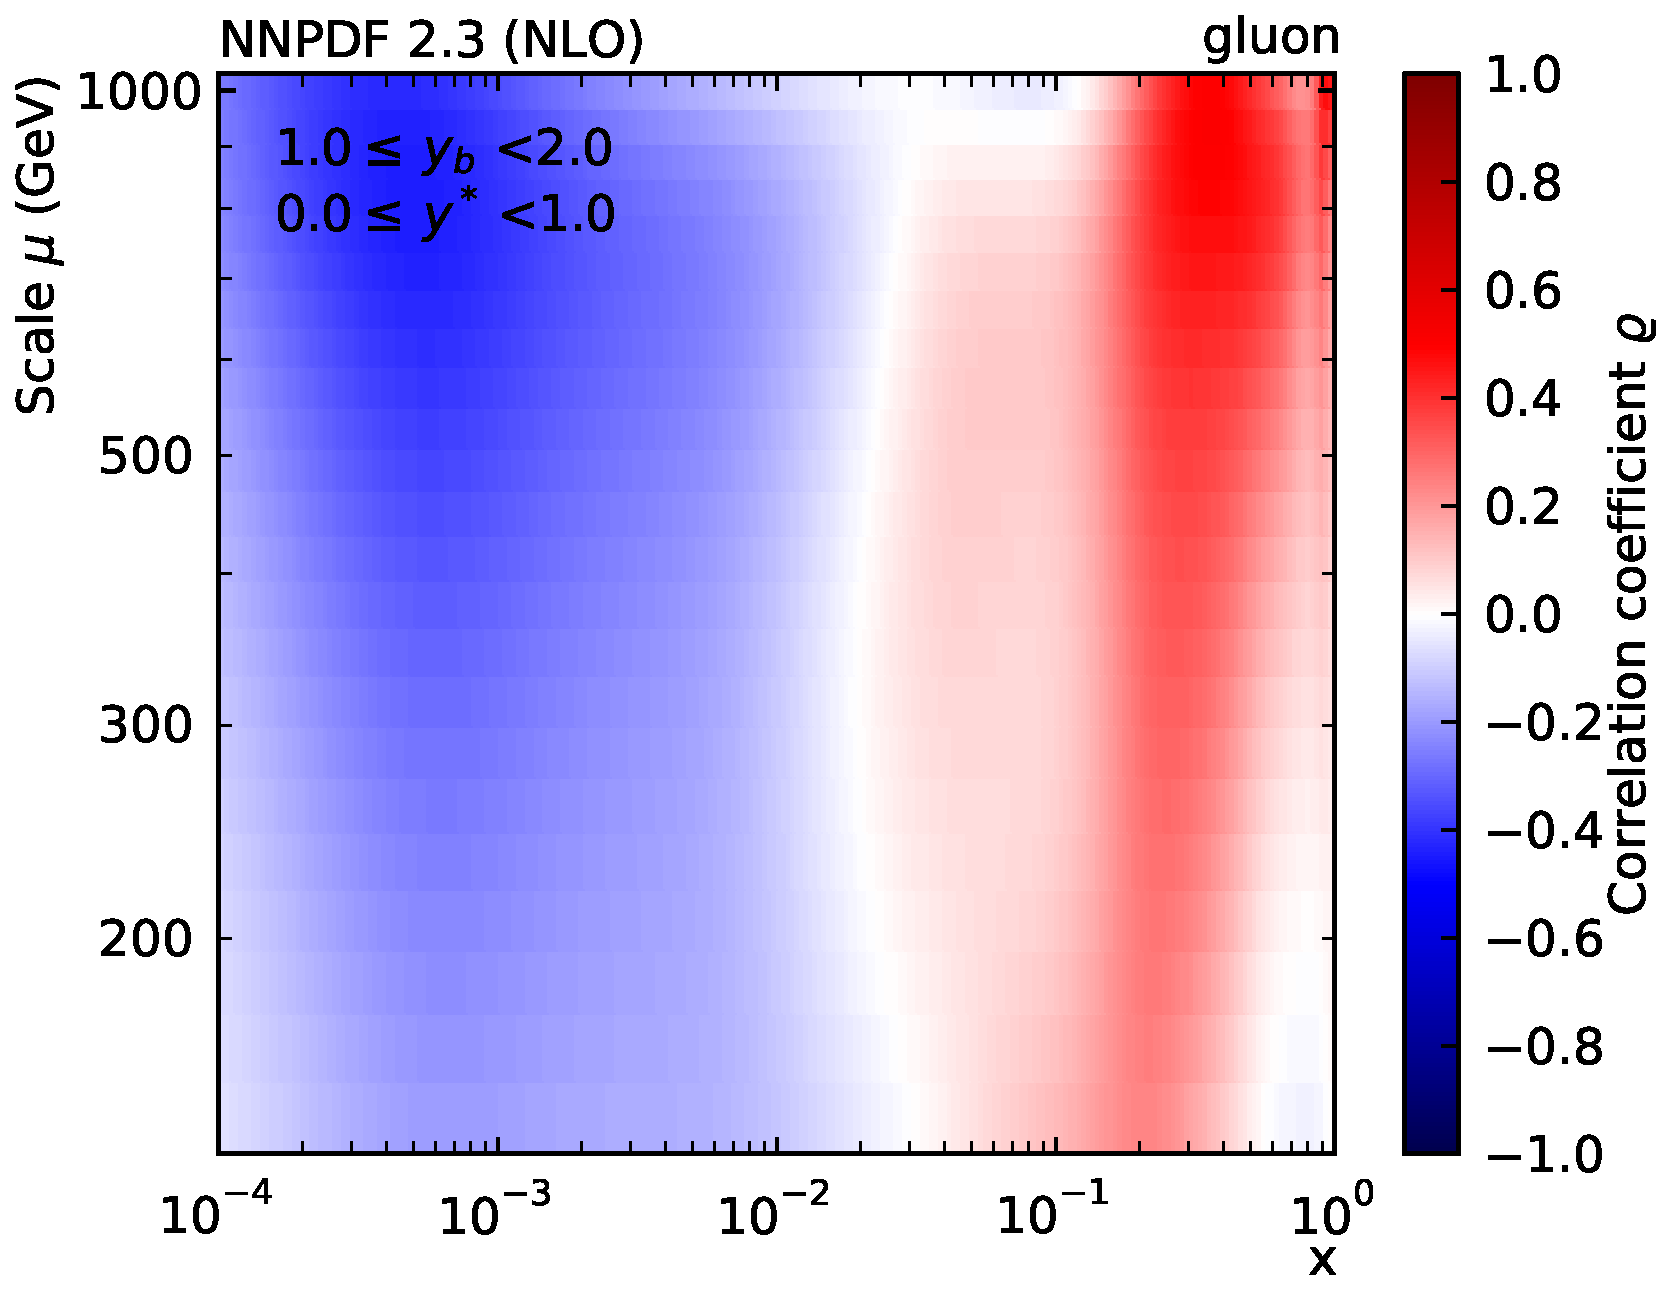
\includegraphics[width=0.49\textwidth]{figures/pdf_constraints/corr_PTMAXEXPYS_YBYS_NLO_FINALBINS_NNPDF23_gluon_ys0_0yb1_0_cl.pdf}\hfill
    \includegraphics[width=0.49\textwidth]{figures/pdf_constraints/corr_PTMAXEXPYS_YBYS_NLO_FINALBINS_NNPDF23_gluon_ys0_0yb2_0_cl.pdf}\hfill
    \includegraphics[width=0.49\textwidth]{figures/pdf_constraints/corr_PTMAXEXPYS_YBYS_NLO_FINALBINS_NNPDF23_gluon_ys1_0yb0_0_cl.pdf}\hfill
    \includegraphics[width=0.49\textwidth]{figures/pdf_constraints/corr_PTMAXEXPYS_YBYS_NLO_FINALBINS_NNPDF23_gluon_ys1_0yb1_0_cl.pdf}\hfill
    \includegraphics[width=0.49\textwidth]{figures/pdf_constraints/corr_PTMAXEXPYS_YBYS_NLO_FINALBINS_NNPDF23_gluon_ys2_0yb0_0_cl.pdf}\hfill
    \caption[Correlation between dijet cross section and gluon PDF]{
            The correlation coefficient between the triple-differential dijet cross
            section and the gluon PDF, as a function of the momentum fraction $x$ of the
            proton and the energy scale $\mu$ of the hard process. The correlation is shown
            for the six bins in \ystar and \yboost of the measurement.}
    \label{fig:pdfconstraints_gluon}
\end{figure}

\begin{figure}[htbp]
    \centering
    \includegraphics[width=0.49\textwidth]{figures/pdf_constraints/corr_PTMAXEXPYS_YBYS_NLO_FINALBINS_NNPDF23_u_valence_quark_ys0_0yb0_0_cl.pdf}\hfill
    \includegraphics[width=0.49\textwidth]{figures/pdf_constraints/corr_PTMAXEXPYS_YBYS_NLO_FINALBINS_NNPDF23_u_valence_quark_ys0_0yb1_0_cl.pdf}\hfill
    \includegraphics[width=0.49\textwidth]{figures/pdf_constraints/corr_PTMAXEXPYS_YBYS_NLO_FINALBINS_NNPDF23_u_valence_quark_ys0_0yb2_0_cl.pdf}\hfill
    \includegraphics[width=0.49\textwidth]{figures/pdf_constraints/corr_PTMAXEXPYS_YBYS_NLO_FINALBINS_NNPDF23_u_valence_quark_ys1_0yb0_0_cl.pdf}\hfill
    \includegraphics[width=0.49\textwidth]{figures/pdf_constraints/corr_PTMAXEXPYS_YBYS_NLO_FINALBINS_NNPDF23_u_valence_quark_ys1_0yb1_0_cl.pdf}\hfill
    \includegraphics[width=0.49\textwidth]{figures/pdf_constraints/corr_PTMAXEXPYS_YBYS_NLO_FINALBINS_NNPDF23_u_valence_quark_ys2_0yb0_0_cl.pdf}\hfill
    \caption[Correlation between dijet cross section and u valence quark PDF]{
            The correlation coefficient between the triple-differential dijet cross
            section and the u valence quark PDF, as a function of the momentum fraction $x$ of the
            proton and the energy scale $\mu$ of the hard process. The correlation is shown
            for the six bins in \ystar and \yboost of the measurement.}

    \label{fig:pdfconstraints_u_valence_quark}
\end{figure}

\begin{figure}[htbp]
    \centering
    \includegraphics[width=0.49\textwidth]{figures/pdf_constraints/corr_PTMAXEXPYS_YBYS_NLO_FINALBINS_NNPDF23_d_valence_quark_ys0_0yb0_0_cl.pdf}\hfill
    \includegraphics[width=0.49\textwidth]{figures/pdf_constraints/corr_PTMAXEXPYS_YBYS_NLO_FINALBINS_NNPDF23_d_valence_quark_ys0_0yb1_0_cl.pdf}\hfill
    \includegraphics[width=0.49\textwidth]{figures/pdf_constraints/corr_PTMAXEXPYS_YBYS_NLO_FINALBINS_NNPDF23_d_valence_quark_ys0_0yb2_0_cl.pdf}\hfill
    \includegraphics[width=0.49\textwidth]{figures/pdf_constraints/corr_PTMAXEXPYS_YBYS_NLO_FINALBINS_NNPDF23_d_valence_quark_ys1_0yb0_0_cl.pdf}\hfill
    \includegraphics[width=0.49\textwidth]{figures/pdf_constraints/corr_PTMAXEXPYS_YBYS_NLO_FINALBINS_NNPDF23_d_valence_quark_ys1_0yb1_0_cl.pdf}\hfill
    \includegraphics[width=0.49\textwidth]{figures/pdf_constraints/corr_PTMAXEXPYS_YBYS_NLO_FINALBINS_NNPDF23_d_valence_quark_ys2_0yb0_0_cl.pdf}\hfill
    \caption[Correlation between dijet cross section and d valence quark PDF]{
            The correlation coefficient between the triple-differential dijet cross
            section and the d valence quark PDF, as a function of the momentum fraction $x$ of the
            proton and the energy scale $\mu$ of the hard process. The correlation is shown
            for the six bins in \ystar and \yboost of the measurement.}
    \label{fig:pdfconstraints_d_valence_quark}
\end{figure}

\begin{figure}[htbp]
    \centering
    \includegraphics[width=0.49\textwidth]{figures/pdf_constraints/corr_PTMAXEXPYS_YBYS_NLO_FINALBINS_NNPDF23_sea_quarks_ys0_0yb0_0_cl.pdf}\hfill
    \includegraphics[width=0.49\textwidth]{figures/pdf_constraints/corr_PTMAXEXPYS_YBYS_NLO_FINALBINS_NNPDF23_sea_quarks_ys0_0yb1_0_cl.pdf}\hfill
    \includegraphics[width=0.49\textwidth]{figures/pdf_constraints/corr_PTMAXEXPYS_YBYS_NLO_FINALBINS_NNPDF23_sea_quarks_ys0_0yb2_0_cl.pdf}\hfill
    \includegraphics[width=0.49\textwidth]{figures/pdf_constraints/corr_PTMAXEXPYS_YBYS_NLO_FINALBINS_NNPDF23_sea_quarks_ys1_0yb0_0_cl.pdf}\hfill
    \includegraphics[width=0.49\textwidth]{figures/pdf_constraints/corr_PTMAXEXPYS_YBYS_NLO_FINALBINS_NNPDF23_sea_quarks_ys1_0yb1_0_cl.pdf}\hfill
    \includegraphics[width=0.49\textwidth]{figures/pdf_constraints/corr_PTMAXEXPYS_YBYS_NLO_FINALBINS_NNPDF23_sea_quarks_ys2_0yb0_0_cl.pdf}\hfill
    \caption[Correlation between dijet cross section and sea quarks PDF]{
            The correlation coefficient between the triple-differential dijet cross
            section and the sea quarks PDF, as a function of the momentum fraction $x$ of the
            proton and the energy scale $\mu$ of the hard process. The correlation is shown
            for the six bins in \ystar and \yboost of the measurement.}
    \label{fig:pdfconstraints_sea_quarks}
\end{figure}

\section{Additional PDF comparisons}


\begin{figure}[tbp]
  \centering
  \includegraphics[width=0.48\textwidth]{figures/pdf_constraints/pdfcomp_direct_0_1.9.pdf}\hfill%
  \includegraphics[width=0.48\textwidth]{figures/pdf_constraints/pdfcomp_direct_9_1.9.pdf}
  \includegraphics[width=0.48\textwidth]{figures/pdf_constraints/pdfcomp_direct_7_1.9.pdf}\hfill%
  \includegraphics[width=0.48\textwidth]{figures/pdf_constraints/pdfcomp_direct_8_1.9.pdf}
  \caption[Direct comparison of gluon and quark PDFs]{The gluon (top left), sea
  quark (top right), d valence quark (bottom left) and u valence quark (bottom
right) PDFs as a function of $x$ as derived from HERA inclusive DIS data
alone (hatched band) and in combination with CMS dijet data (solid band). The PDFs
are shown at the starting scale $Q^2 = \SI{1.9}{\GeV \squared}$. The total
uncertainty of the PDFs is shown.}
  \label{fig:pdfconstraints:direct:19}
\end{figure}

\begin{figure}[tbp]
  \centering
  \includegraphics[width=0.48\textwidth]{figures/pdf_constraints/pdfcomp_direct_0_10000.pdf}\hfill%
  \includegraphics[width=0.48\textwidth]{figures/pdf_constraints/pdfcomp_direct_9_10000.pdf}
  \includegraphics[width=0.48\textwidth]{figures/pdf_constraints/pdfcomp_direct_7_10000.pdf}\hfill%
  \includegraphics[width=0.48\textwidth]{figures/pdf_constraints/pdfcomp_direct_8_10000.pdf}
  \caption[Direct comparison of gluon and quark PDFs]{The gluon (top left), sea
  quark (top right), d valence quark (bottom left) and u valence quark (bottom
right) PDFs as a function of $x$ as derived from HERA inclusive DIS data
alone (hatched band) and in combination with CMS dijet data (solid band). The PDFs
are evolved to the scale $Q^2 = \SI{10000}{\GeV \squared}$. The total
uncertainty of the PDFs is shown.}
\label{fig:pdfconstraints:direct:10000}
\end{figure}
